% Options for packages loaded elsewhere
\PassOptionsToPackage{unicode}{hyperref}
\PassOptionsToPackage{hyphens}{url}
%
\documentclass[
]{book}
\usepackage{amsmath,amssymb}
\usepackage{lmodern}
\usepackage{iftex}
\ifPDFTeX
  \usepackage[T1]{fontenc}
  \usepackage[utf8]{inputenc}
  \usepackage{textcomp} % provide euro and other symbols
\else % if luatex or xetex
  \usepackage{unicode-math}
  \defaultfontfeatures{Scale=MatchLowercase}
  \defaultfontfeatures[\rmfamily]{Ligatures=TeX,Scale=1}
\fi
% Use upquote if available, for straight quotes in verbatim environments
\IfFileExists{upquote.sty}{\usepackage{upquote}}{}
\IfFileExists{microtype.sty}{% use microtype if available
  \usepackage[]{microtype}
  \UseMicrotypeSet[protrusion]{basicmath} % disable protrusion for tt fonts
}{}
\makeatletter
\@ifundefined{KOMAClassName}{% if non-KOMA class
  \IfFileExists{parskip.sty}{%
    \usepackage{parskip}
  }{% else
    \setlength{\parindent}{0pt}
    \setlength{\parskip}{6pt plus 2pt minus 1pt}}
}{% if KOMA class
  \KOMAoptions{parskip=half}}
\makeatother
\usepackage{xcolor}
\usepackage{color}
\usepackage{fancyvrb}
\newcommand{\VerbBar}{|}
\newcommand{\VERB}{\Verb[commandchars=\\\{\}]}
\DefineVerbatimEnvironment{Highlighting}{Verbatim}{commandchars=\\\{\}}
% Add ',fontsize=\small' for more characters per line
\usepackage{framed}
\definecolor{shadecolor}{RGB}{248,248,248}
\newenvironment{Shaded}{\begin{snugshade}}{\end{snugshade}}
\newcommand{\AlertTok}[1]{\textcolor[rgb]{0.94,0.16,0.16}{#1}}
\newcommand{\AnnotationTok}[1]{\textcolor[rgb]{0.56,0.35,0.01}{\textbf{\textit{#1}}}}
\newcommand{\AttributeTok}[1]{\textcolor[rgb]{0.77,0.63,0.00}{#1}}
\newcommand{\BaseNTok}[1]{\textcolor[rgb]{0.00,0.00,0.81}{#1}}
\newcommand{\BuiltInTok}[1]{#1}
\newcommand{\CharTok}[1]{\textcolor[rgb]{0.31,0.60,0.02}{#1}}
\newcommand{\CommentTok}[1]{\textcolor[rgb]{0.56,0.35,0.01}{\textit{#1}}}
\newcommand{\CommentVarTok}[1]{\textcolor[rgb]{0.56,0.35,0.01}{\textbf{\textit{#1}}}}
\newcommand{\ConstantTok}[1]{\textcolor[rgb]{0.00,0.00,0.00}{#1}}
\newcommand{\ControlFlowTok}[1]{\textcolor[rgb]{0.13,0.29,0.53}{\textbf{#1}}}
\newcommand{\DataTypeTok}[1]{\textcolor[rgb]{0.13,0.29,0.53}{#1}}
\newcommand{\DecValTok}[1]{\textcolor[rgb]{0.00,0.00,0.81}{#1}}
\newcommand{\DocumentationTok}[1]{\textcolor[rgb]{0.56,0.35,0.01}{\textbf{\textit{#1}}}}
\newcommand{\ErrorTok}[1]{\textcolor[rgb]{0.64,0.00,0.00}{\textbf{#1}}}
\newcommand{\ExtensionTok}[1]{#1}
\newcommand{\FloatTok}[1]{\textcolor[rgb]{0.00,0.00,0.81}{#1}}
\newcommand{\FunctionTok}[1]{\textcolor[rgb]{0.00,0.00,0.00}{#1}}
\newcommand{\ImportTok}[1]{#1}
\newcommand{\InformationTok}[1]{\textcolor[rgb]{0.56,0.35,0.01}{\textbf{\textit{#1}}}}
\newcommand{\KeywordTok}[1]{\textcolor[rgb]{0.13,0.29,0.53}{\textbf{#1}}}
\newcommand{\NormalTok}[1]{#1}
\newcommand{\OperatorTok}[1]{\textcolor[rgb]{0.81,0.36,0.00}{\textbf{#1}}}
\newcommand{\OtherTok}[1]{\textcolor[rgb]{0.56,0.35,0.01}{#1}}
\newcommand{\PreprocessorTok}[1]{\textcolor[rgb]{0.56,0.35,0.01}{\textit{#1}}}
\newcommand{\RegionMarkerTok}[1]{#1}
\newcommand{\SpecialCharTok}[1]{\textcolor[rgb]{0.00,0.00,0.00}{#1}}
\newcommand{\SpecialStringTok}[1]{\textcolor[rgb]{0.31,0.60,0.02}{#1}}
\newcommand{\StringTok}[1]{\textcolor[rgb]{0.31,0.60,0.02}{#1}}
\newcommand{\VariableTok}[1]{\textcolor[rgb]{0.00,0.00,0.00}{#1}}
\newcommand{\VerbatimStringTok}[1]{\textcolor[rgb]{0.31,0.60,0.02}{#1}}
\newcommand{\WarningTok}[1]{\textcolor[rgb]{0.56,0.35,0.01}{\textbf{\textit{#1}}}}
\usepackage{longtable,booktabs,array}
\usepackage{calc} % for calculating minipage widths
% Correct order of tables after \paragraph or \subparagraph
\usepackage{etoolbox}
\makeatletter
\patchcmd\longtable{\par}{\if@noskipsec\mbox{}\fi\par}{}{}
\makeatother
% Allow footnotes in longtable head/foot
\IfFileExists{footnotehyper.sty}{\usepackage{footnotehyper}}{\usepackage{footnote}}
\makesavenoteenv{longtable}
\usepackage{graphicx}
\makeatletter
\def\maxwidth{\ifdim\Gin@nat@width>\linewidth\linewidth\else\Gin@nat@width\fi}
\def\maxheight{\ifdim\Gin@nat@height>\textheight\textheight\else\Gin@nat@height\fi}
\makeatother
% Scale images if necessary, so that they will not overflow the page
% margins by default, and it is still possible to overwrite the defaults
% using explicit options in \includegraphics[width, height, ...]{}
\setkeys{Gin}{width=\maxwidth,height=\maxheight,keepaspectratio}
% Set default figure placement to htbp
\makeatletter
\def\fps@figure{htbp}
\makeatother
\setlength{\emergencystretch}{3em} % prevent overfull lines
\providecommand{\tightlist}{%
  \setlength{\itemsep}{0pt}\setlength{\parskip}{0pt}}
\setcounter{secnumdepth}{5}
\newlength{\cslhangindent}
\setlength{\cslhangindent}{1.5em}
\newlength{\csllabelwidth}
\setlength{\csllabelwidth}{3em}
\newlength{\cslentryspacingunit} % times entry-spacing
\setlength{\cslentryspacingunit}{\parskip}
\newenvironment{CSLReferences}[2] % #1 hanging-ident, #2 entry spacing
 {% don't indent paragraphs
  \setlength{\parindent}{0pt}
  % turn on hanging indent if param 1 is 1
  \ifodd #1
  \let\oldpar\par
  \def\par{\hangindent=\cslhangindent\oldpar}
  \fi
  % set entry spacing
  \setlength{\parskip}{#2\cslentryspacingunit}
 }%
 {}
\usepackage{calc}
\newcommand{\CSLBlock}[1]{#1\hfill\break}
\newcommand{\CSLLeftMargin}[1]{\parbox[t]{\csllabelwidth}{#1}}
\newcommand{\CSLRightInline}[1]{\parbox[t]{\linewidth - \csllabelwidth}{#1}\break}
\newcommand{\CSLIndent}[1]{\hspace{\cslhangindent}#1}
\ifLuaTeX
  \usepackage{selnolig}  % disable illegal ligatures
\fi
\IfFileExists{bookmark.sty}{\usepackage{bookmark}}{\usepackage{hyperref}}
\IfFileExists{xurl.sty}{\usepackage{xurl}}{} % add URL line breaks if available
\urlstyle{same} % disable monospaced font for URLs
\hypersetup{
  pdftitle={Adaptations et Interactions gestuelles et haptiques, ciblées utilisateurs. Vers plus d'utilisabilité et d'accessibilité},
  pdfauthor={Bertrand Tornil},
  hidelinks,
  pdfcreator={LaTeX via pandoc}}

\title{Adaptations et Interactions gestuelles et haptiques, ciblées utilisateurs.
Vers plus d'utilisabilité et d'accessibilité}
\author{Bertrand Tornil}
\date{2023-01-12}

\begin{document}
\maketitle

{
\setcounter{tocdepth}{1}
\tableofcontents
}
\hypertarget{preface}{%
\chapter*{Preface}\label{preface}}
\addcontentsline{toc}{chapter}{Preface}

Avec les interfaces graphiques à manipulation directe,
l'utilisateur interagit avec l'ordinateur à l'aide d'un écran, d'un
dispositif de pointage (généralement une souris) et d'un clavier. Ces
interfaces sont faciles à apprendre et à utiliser, grâce à une spatialisation
de l'information qui réduit la charge cognitive de l'utilisateur. Toutefois,
ce schéma d'interaction est incomplet~: il exclut notamment les utilisateurs
non-voyants. Aussi, dans ce cas, l'utilisation du retour de force peut aider
en palliant, autant que raisonnablement possible, à l'absence du canal
visuel.

Dans ce travail de thèse, nous nous sommes intéressés au retour de force,
ainsi qu'à ces applications dans les systèmes interactifs.

Le système tactilo-kinesthésique ou «~haptique~» est la synthèse des
mouvements d'exploration du système moteur (les mouvements) et des
perceptions tactiles (le sens du toucher) et kinesthésiques (la connaissance
que l'on a des positions et mouvements de notre corps et de nos membres).
Ainsi, le système haptique permet de percevoir, et d'agir sur notre
environnement.

Parallèlement à cette dualité, nous avons considéré ces deux aspects selon
deux approches.

Dans une première approche, nous utilisons un système à retour de force
pour essayer d'améliorer les temps lors d'une tâche de pointage. Il nous est
apparu que le retour de force était un élément distracteur. Les temps de
pointage se sont écroulés de 25\% lors d'une première expérience. Par la
suite, nous avons montré lors d'une deuxième expérience, qu'en modulant
l'intensité du retour d'effort selon l'inverse de la vitesse, il était
possible d'améliorer cette situation.

Dans une deuxième approche, nous avons défini un contexte d'utilisation de
périphériques de pointage à retour de force dans un cadre d'accéssiblité des
personnes non-voyantes à certains documents graphiques~: il s'agit de la
«~localisation relative~». Dans ce contexte d'utilisation, il est question de
se reconstruire une image mentale de ce qu'il y a d'affiché à l'écran, sans
la modalité visuelle. Nous avons ensuite développé des prototypes appliquant
la localisation relative dans les domaines de la géographie, de l'anatomie et
de l'harmonie musicale. Ceci nous a amené à créer une série de classes
génériques permettant la générations des documents nécessaires à
l'utilisation de nos périphériques, dans un contexte d'application orientée
Web~: les documents graphiques utilisent le formalisme XML (SVG pour la 2D et
X3D pour la 3D), et une architecture client-serveur est mise en place~: le
serveur Web Apache, exécutant des scripts php ou perl, eux-mêmes générant les
documents et les médias.

Thèse soutenue le 8 décembre 2006, devant le jury composé de~:

\begin{itemize}
\tightlist
\item
  Noëlle Carbonell, Rapporteur
\item
  Jaime Lopez Krahe, Rapporteur
\item
  Dominique Archambault, Examinateur
\item
  Philippe Palanque, Examinateur
\item
  Florence Sedes, Examinateur
\item
  Monique Truquet, Membre invité
\item
  Nadine Baptiste-Jessel, Directrice de thèse
\end{itemize}

\hypertarget{entruxe9e-bibtex}{%
\section*{Entrée bibtex}\label{entruxe9e-bibtex}}
\addcontentsline{toc}{section}{Entrée bibtex}

\begin{Shaded}
\begin{Highlighting}[]
\VariableTok{@phdthesis}\NormalTok{\{}\OtherTok{tornil2006adaptations}\NormalTok{,}
  \DataTypeTok{title}\NormalTok{=\{Adaptations et interactions gestuelles et haptiques, cibl\{}\CharTok{\textbackslash{}\textquotesingle{}}\NormalTok{e\}es utilisateurs: vers plus d\textquotesingle{}utilisabilit\{}\CharTok{\textbackslash{}\textquotesingle{}}\NormalTok{e\} et d\textquotesingle{}accessibilit\{}\CharTok{\textbackslash{}\textquotesingle{}}\NormalTok{e\}\},}
  \DataTypeTok{author}\NormalTok{=\{Tornil, Bertrand\},}
  \DataTypeTok{year}\NormalTok{=\{2006\},}
  \DataTypeTok{month}\NormalTok{ = \{décembre\},}
  \DataTypeTok{url}\NormalTok{ = \{https://www.tornil.me/these/\},}
  \DataTypeTok{type}\NormalTok{ = \{Thèse de doctorat\},}
  \DataTypeTok{school}\NormalTok{=\{Toulouse 3\}}
  \DataTypeTok{address}\NormalTok{ = \{Toulouse, France\},}
  \DataTypeTok{language}\NormalTok{ = \{français\}}
\NormalTok{\}}
\end{Highlighting}
\end{Shaded}

\hypertarget{remerciements}{%
\section*{Remerciements}\label{remerciements}}
\addcontentsline{toc}{section}{Remerciements}

Ca y est, c'est l'heure des remerciements. Pour un lecteur, cette page est
tout au début de ce document. Mais pour moi, ce sont les derniers mots que je
vais y ajouter, cinq années après avoir débuté l'aventure.

Je remercie tout d'abord mes, rapporteurs, les professeurs Noëlle Carbonell
et Jaime Lopez Krahe, pour leur patience, et leurs précieuses remarques sur
mon travail. Je remercie également les autres membres du jury, Florence
Sedes, Philippe Palanque et Dominique Archambault, qui ont accepté de prendre
sur leurs temps pour participer à ma soutenance.

Je présente ici toute ma gratitude à Nadine Baptiste-Jessel, ma directrice
de thèse, qui m'aura aidé à finalement achever cette thèse, même à 400 km de
distance. Un grand merci, également au reste de l'équipe~: Dany et Benoît,
pour tous ces instants. Un merci tout spécial à Monique Truquet, pour sa
précieuse relecture.

Cinq ans, ce sont des rencontres au sein de l'université. Machine à café
et refaisage de monde avec Romain, Laurent, Cédric, Amélie, Fred\ldots{} Mais
aussi ouverture sur d'autres domaines de la recherche\ldots{}

Cinq ans, ce sont des rencontres hors de l'université. Merci à Matthieu,
Tony, Lionel, Benj, Xavier et Vincent, pour la vie toulousaine ; merci à
Arnaud, Christelle, David, Hervé, Charlot, Alex, Didier, Filou, Jay,
Moustique, Pipi, Vivie, et à tout ceux du berry que j'oublie\ldots{}

Cinq ans, c'est trop long pour un financement classique de thèse. Aussi,
j'ai été amené à travailler pour la terminer. Et ce sont des nouvelles
rencontres, qui marquent, elles aussi~: Seb, Greg, Corinne, Karine et Alex de
WS-Interactive. Et comme cinq ans, c'est vraiment trop long, je suis déjà
dans un autre cadre professionnel aujourd'hui, et je remercie déjà pour la
suite Alain, Solange et Paul de UIXperts.

Cinq ans, enfin, c'est déjà une bonne tranche de vie. Il y a cinq ans, la
famille, c'était surtout mon père~: Merci papa\ldots{} pour tout\ldots{} Et depuis, il
y a eu la rencontre avec ma douce et tendre Ariane, qui, cette année, a passé
le plus bel examen qui soit, en donnant naissance à Sasha, notre petite
louloute.

\begin{quote}
Il était un aveugle qui cherchait son chemin,

Et prenait repères de son oreille et de sa main.

Il demandait aux passants qu'il rencontrait,

De décrire séant objets et actions qu'eux voyaient.

Mais rien n'y fit vraiment car les indices qu'il reçut,

Remplaçaient difficilement sa vue perdue.

Ailleurs se promenait un astronaute,

Qui voyait parfaitement et sans faute,

Il consultait sa carte, sans peine ni effort,

Et savait d'avance trouver son chemin en dehors.

Mais ses membres sans poids au gré du vent allaient

Contre sa volonté pourtant fort développée.

Finalement il n'eut de meilleur choix que de demander,

Au passant aveugle qu'il rencontrât,

Si ce dernier pouvait lui prêter,

le temps d'un pas,

Une main ferme et un pied assuré.

Ensemble ils découvrirent l'art de conjuguer

Ce qu'avant ils ne faisaient que regretter.

Ramstein, La métaphore de l'astronaute et de l'aveugle, 1995
\end{quote}

\hypertarget{introduction}{%
\chapter*{Introduction}\label{introduction}}
\addcontentsline{toc}{chapter}{Introduction}

L'informatique désigne l'automatisation du traitement de l'information par
un système \footnote{\url{http://fr.wikipedia.org/wiki/Informatique}}.

Une partie de ces traitements est de plus en plus réalisée au sein même de
nos salons, dans nos maisons~; il s'agit de l'informatique personnelle. Dans
ce contexte, les traitements effectués par le système doivent généralement
fournir une réponse à la personne qui utilise ce système~; personne que nous
appellerons utilisateur dans toute la suite de ce document.

Maintenant, nous avons un système et un utilisateur. Nous pouvons à
présent nous demander comment le second utilise le premier\ldots{} et comment le
premier répond au second. C'est cette démarche de questionnement qui
sous-tend le domaine de l'interaction Homme-Machine (ou IHM, ou HCI en
anglais).

Dans le sens machine-humain, l'interaction est produite par les
dispositifs de sortie, tels que l'écran, ou plus indirectement, par
l'imprimante. Dans le sens opposé, c'est à dire humain-machine, on se sert
généralement d'un clavier et d'une souris, mais comme nous le verrons, il
existe bien d'autres dispositifs permettant d'agir sur la machine. Et dans
cette thèse, nous étudierons plus précisément le matériel d'interaction, basé
sur le sens du toucher, et des mouvements.

Nous pourrons alors nous poser la question suivante~: quels problèmes
apparaissent lorsque l'utilisateur ne peut pas voir l'écran, soit à cause
d'un handicap perceptif, soit parce que la vue est monopolisée par une autre
tâche~? Et comment un dispositif basé sur les sens du toucher et du
mouvement peut-il être utilisé dans un tel contexte, que peut-il amener, et
quelles en sont les limites~?

La première partie de ce document est focalisée sur l'interaction
Homme-Machine mettant en œuvre le retour de force ou les sensation tactiles,
et elle pose l'état de l'art. Pour commencer nous étudions dans le chapitre 2
(le premier chapitre étant cette introduction) le côté humain de ces
perceptions, en nous intéressant notamment aux neurosciences. Nous parlerons
au chapitre 3 des communications homme-machine proprement dites, depuis les
principales définitions, jusqu'aux applications de l'interaction haptique,
tout en ayant détaillé les moyens techniques d'interaction. Le quatrième
chapitre de cette thèse proposera alors une utilisation du retour de force
visant à améliorer les performances d'une tâche de pointage.

La deuxième partie de cette thèse traite des possibilités du retour de
force en terme d'accessibilité, avec dans le chapitre 5, les principales
définitions et réalisations de ce domaine. Le chapitre 6 introduit alors mes
propositions~: un contexte d'utilisation des dispositifs de pointage à retour
de force~: la localisation relative. Nous appliquerons alors cette approche à
l'apprentissage de cartes géographiques, ou d'accords de musique.

Nous conclurons alors, et dresserons les perspectives possibles à ces
travaux.

\hypertarget{part-lhomme-et-la-machine-interactions}{%
\part{L'homme et la machine : interactions}\label{part-lhomme-et-la-machine-interactions}}

\hypertarget{le-systuxe8me-haptique-de-lhomme}{%
\chapter{Le système haptique de l'homme}\label{le-systuxe8me-haptique-de-lhomme}}

\hypertarget{introduction-1}{%
\section{Introduction}\label{introduction-1}}

\hypertarget{nos-sens-et-la-perception-du-monde}{%
\subsection{Nos sens et la perception du monde}\label{nos-sens-et-la-perception-du-monde}}

Avant d'aborder plus spécifiquement le sujet qui nous intéresse, nous
allons passer en revue quelques classifications des systèmes de la perception
humaine.

Il est d'usage de parler des cinq sens~: la vue, l'ouïe, l'odorat, le goût
et le toucher. Cette classification constitue une première approche de la
perception du monde qui nous entoure~; comme nous allons le voir, la
perception est bien plus complexe.

Pour commencer, j'ai choisi de citer le résultat d'une étude en
psychologie (\protect\hyperlink{ref-turbiaux1996richelle}{Turbiaux, 1996}) qui a abordé
le problème de la perception des informations. Selon cette étude, ces
dernières sont perçues par un sujet voyant à:

\begin{itemize}
\tightlist
\item
  83 \% par la vision~;
\item
  11\% par l'audition~;
\item
  3,5\% par l'odorat~;
\item
  1,5\% par le toucher~;
\item
  et 1\% par le goût.
\end{itemize}

Pour autant, il faut rester prudent avec une telle approche. En effet, la
perception \emph{peut} être segmentée en cinq sens. Pourtant, le
tableau \ref{tab:perception} présente une classification
des sensations. Il s'agit de la classification de Sherrington
(1857-1952).

\begin{longtable}[]{@{}l@{}}
\caption{\label{tab:perception} Classification des sensations de Sherrington
(\protect\hyperlink{ref-calas2016precis}{Calas et al., 2016})}\tabularnewline
\toprule()
\endhead
\bottomrule()
\end{longtable}

les extérocepteurs~:
nous renseignent sur le monde extérieur

télérécepteurs~:
perception à distance

récepteurs visuels

récepteurs auditifs

récepteurs olfactifs

récepteurs de
contact

récepteurs gustatifs

récepteurs cutanés du toucher

les
intérocepteurs~: nous renseignent sur notre propre organisme

viscérocepteurs~:
disséminés dans les viscères

nous renseignent sur un paramètre
physiologique interne (la douleur par exemple)

propriocepteurs~:
regroupés (oreille interne) ou disséminés (fuseaux
neuro-musculaires)

nous renseignent sur un paramètre lié
au travail de relation~: l'état de tension des muscles, sur la
position relative des différentes parties du corps, et sur la
position du corps dans l'espace

Étudions plus précisément tout ce vocabulaire\ldots{}

\textbf{La~sensibilité~intéroceptive~:}

Elle comprend toutes les sensations qui viennent
de l'estomac, de l'intestin. S'y ajoutent les sensations viscérales, ainsi
que cette sensibilité générale du corps qu'on appelle la coenesthésie
(sensations d'aise ou de malaise).

\textbf{La~sensibilité~proprioceptive~:}

Celle qui nous renseigne sur les positions, attitudes, mouvements de
notre corps et de nos membres. Cette sensibilité comprend~:

\begin{enumerate}
\def\labelenumi{\arabic{enumi}.}
\tightlist
\item
  le sens kinésique ou kinesthésique~: il nous
  renseigne sur nos mouvements proprement dits (déplacements de nos
  membres et de notre corps dans l'espace)~;
\item
  le sens statique ou vestibulaire~: sens qui a
  son organe dans l'oreille interne et qui nous donne le sens de la
  verticalité, des mouvements de rotation et de translation~; il préside à
  l'équilibration générale du corps.
\end{enumerate}

\textbf{La~sensibilité~extéroceptive~:}

Elle nous informe sur les objets extérieurs. Les psychologues
distinguaient les sens impressionnables par contact direct et les sens
qui sont impressionnables à distance.

\begin{enumerate}
\def\labelenumi{\arabic{enumi}.}
\tightlist
\item
  Les sens impressionnables par contact direct~:

  \begin{enumerate}
  \def\labelenumii{\arabic{enumii}.}
  \tightlist
  \item
    Les sensibilités cutanées~: le toucher qui
    suppose un contact direct avec l'objet à percevoir

    \begin{itemize}
    \tightlist
    \item
      le tact,
    \item
      les sensations thermiques,
    \item
      la douleur.
    \end{itemize}
  \item
    Les sens chimiques~: le goût et l'odorat
    liés aux fonctions de nutrition.
  \end{enumerate}
\item
  Les sens impressionnables à distance~: Ces sens
  sont plus indépendants du milieu extérieur que ceux qui exigent le
  contact direct. L'ouïe et la vue apportent à l'être vivant des messages
  lointains qui lui permettent une adaptation anticipée de son
  comportement.
\end{enumerate}

Pour (\protect\hyperlink{ref-berthoz1997sens}{Berthoz, 1997}), «~la
perception n'est pas seulement une interprétation des messages sensoriels.
Elle est également contrainte par l'action, simulation interne de l'action,
jugement et prise de décision et anticipation des conséquences de l'action~:
il y a filtrage des informations données par les sens en fonction de ses
projets propres. Un très grand nombre de mouvements exigent une anticipation
ou une extrapolation fondée sur une estimation utilisant les expériences
antérieures (rôle de la mémoire).~»

Tout ceci nous donne une vision peu évidente de la perception. Et il n'est
pas question ici d'aborder le côté philosophique de la question.

\begin{quote}
«~Percevoir, c'est se rendre quelque chose de présent à l'aide du corps~»

Merleau-Ponty
\end{quote}

Pour finir cette partie d'introduction, précisons que toutes les
connaissances qui se rapportent au corps, évoluent en fonction des avancées
de la compréhension des mécanismes mis en œuvre.

Nous allons tenter, dans ce qui suit, de définir la terminologie utilisée
lorsqu'il est question d'interaction haptique.

\hypertarget{premiuxe8re-approche-du-systuxe8me-haptique}{%
\subsection{Première approche du système haptique}\label{premiuxe8re-approche-du-systuxe8me-haptique}}

\begin{quote}
Our knowledge of touch consists of only fragmentary concepts and findings,
some dealing with basic functional properties (e.g., cutaneous sensitivity,
limits of kinaesthetic space perception) and others with capabilities of
the systems as a whole (e.g., the identification of three-dimensional
objects)

(\protect\hyperlink{ref-loomis1986tactual}{Loomis and Lederman, 1986}), cité par
(\protect\hyperlink{ref-colwell2001non}{Colwell, 2001})
\end{quote}

Tout d'abord, un petit peu d'étymologie. Le mot haptique vient du grec
\emph{haptestai} signifiant «~toucher~», et
est originalement synonyme au sens tactile.

D'après (\protect\hyperlink{ref-appelle2013haptic}{Appelle, 2013}), ce serait le
psychologue (\protect\hyperlink{ref-revesz1950psychology}{Révész, 1950}) qui aurait le
premier utilisé le terme haptique pour désigner le système
tactilo-kinesthésique de la main, c'est à dire la synthèse

\begin{enumerate}
\def\labelenumi{\arabic{enumi}.}
\tightlist
\item
  des perceptions des systèmes sensoriels de la
  main
\item
  et des mouvements d'exploration de la main.
\end{enumerate}

Plus tard, pour \href{047-bibliographie.html\#Loomis1986}{(Loomis et Lederman,
1986)}, la perception haptique était celle qui impliquait les sens cutanés
et kinesthésiques pour transmettre l'information sur un objet ou sur un
évènement. Ils n'ont cependant pas restreint cette définition à la main. La
sensation de la texture de la nourriture dans la bouche apparaît donc comme
une partie de la perception haptique, au sens de Loomis et Lerdeman.

Une autre définition est celle de \href{047-bibliographie.html\#Gibson1966}{(Gibson,
1966)} (toujours cité par \href{047-bibliographie.html\#Appelle1991}{(Appelle,
1991)}). Pour lui, la pression, la force, la stimulation de la peau,
l'activité des muscles, des articulations et des tendons étaient mises en
œuvre lors de la manipulation d'objets. Pour Gibson, le système haptique
inclue plusieurs sous-systèmes~:

\begin{itemize}
\tightlist
\item
  Le toucher cutané: une stimulation de la peau sans
  mouvements des muscles ou des articulations.
\item
  Le toucher haptique~: une stimulation de la peau avec
  des mouvements des articulations.
\item
  Le toucher dynamique~: une stimulation de la peau
  avec des mouvements des articulations et des muscles.
\item
  Le toucher orienté: une stimulation de la peau avec
  une stimulation vestibulaire \footnote{relatif notamment au sens de l'équilibre}.
\end{itemize}

(\protect\hyperlink{ref-appelle2013haptic}{Appelle, 2013}) a très justement noté
que la prolifération des termes et des définitions liés à la perception
haptique, indique que la compréhension dans ce domaine n'en est toujours qu'à
ces débuts. Il est également fréquent de trouver des définitions
contradictoires entre plusieurs recueils.

Dans ce chapitre et dans la suite de cette thèse, nous retiendrons la
définition actuellement admise, à savoir~:

le terme haptique
se réfère à la combinaison~:

\begin{enumerate}
\def\labelenumi{\arabic{enumi}.}
\tightlist
\item
  \protect\hyperlink{somesthesie}{du système perceptif lié au toucher et à la
  kinesthésie},
\item
  \protect\hyperlink{moteur}{et des mouvements d'exploration}.
\end{enumerate}

\hypertarget{somesthesie}{%
\section{Le système haptique côté perception~: la somesthésie}\label{somesthesie}}

La somesthésie est liée à l'ensemble des sensibilités cutanées et
internes. Elle est composé par~:

\begin{itemize}
\tightlist
\item
  \textbf{le~sens~tactile}: il est relayé par
  les récepteurs sensoriels situés sous l'épiderme, et dont on relève la plus
  grande densité dans la main. Ces récepteurs relaient «~le contact
  initial avec l'environnement~», et permettent d'en appréhender la
  géométrie détaillée de la surface, la rugosité, la température (toujours de
  surface).
\item
  \textbf{le~sens~kinesthésique}: du grec
  \emph{kinêsin} signifiant «~se mouvoir~» et
  \emph{aisthêsis} signifiant sensation , il se réfère à
  la kinesthésie, la sensation interne du mouvement des parties du corps
  assurée par le sens musculaire (sensibilité profonde des muscles) et par
  les excitations de l'oreille interne {[}Le Petit Robert{]}. Ce sens permet de
  connaître l'effort que font nos muscles par exemple lorsque nous soulevons
  (poids) ou lorsque nous poussons (résistance) un objet.
\end{itemize}

\hypertarget{la-perception-tactile}{%
\subsection{La perception tactile}\label{la-perception-tactile}}

Les récepteurs physiologiques de la perception tactile se trouvent dans la
peau \ref{fig:Structure-de-la}. La bande passante
du sens tactile (c'est à dire la fréquence à laquelle les stimuli tactiles
sont perçus) et de 0 à 400 Hz (\href{047-bibliographie.html\#Shimoga1992}{Shimoga,
1992}). Elle peut cependant monter à des très hautes fréquences situées
entre 5000 à 10000 Hz dans le cas de la reconnaissance de textures à très
petits détails.

\begin{figure}
\centering
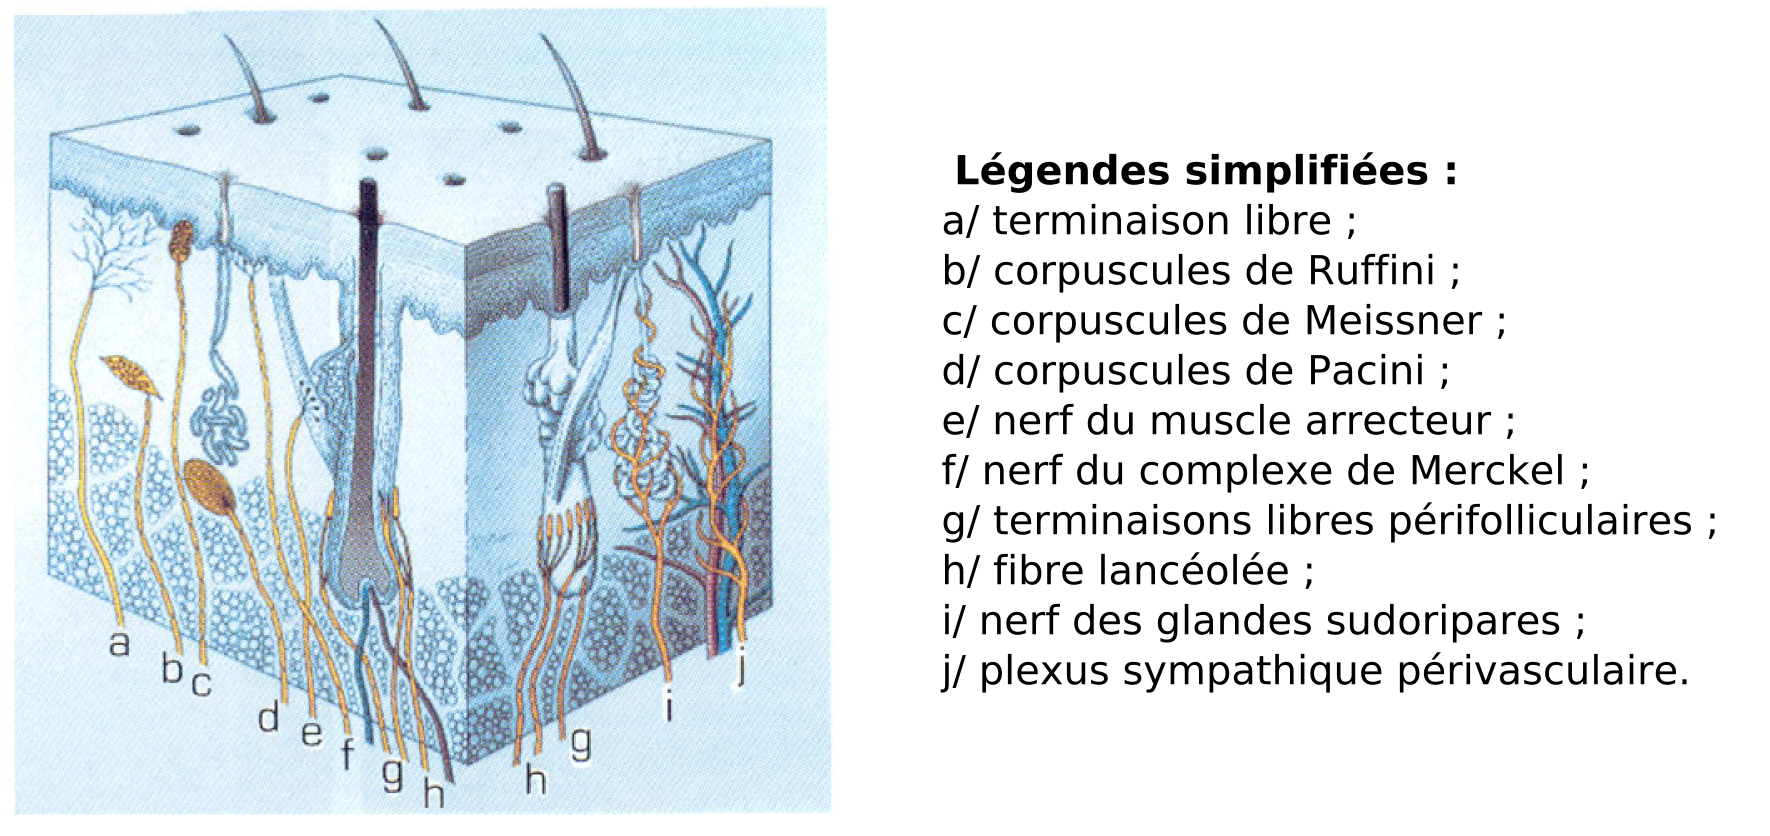
\includegraphics{img/peau.png}
\caption{\label{fig:Structure-de-la} Structure de la
peau (emprunté à (\protect\hyperlink{ref-reznik1996structure}{Reznik, 1996}))}
\end{figure}

Nous pouvons distinguer 3 natures de récepteurs tactiles~:

\begin{itemize}
\tightlist
\item
  les thermorécepteurs~: liés aux sensations de chaud et de froid~;
\item
  les nocirécepteurs~: liés à la sensation de douleur~;
\item
  les mécanorécepteurs~: liés à la discrimination tactile.
\end{itemize}

On distingue 4 types de mécanorécepteurs (\protect\hyperlink{ref-cholewiak2013sensory}{Cholewiak and Collins, 2013}),
(\protect\hyperlink{ref-kalawsky1993science}{Kalawsky, 1993}), (\protect\hyperlink{ref-seow1988physiology}{Seow, 1988})~; Il sont présentés dans le
tableau \ref{tab:tactile}.

\begin{longtable}[]{@{}
  >{\raggedright\arraybackslash}p{(\columnwidth - 10\tabcolsep) * \real{0.1645}}
  >{\raggedright\arraybackslash}p{(\columnwidth - 10\tabcolsep) * \real{0.1250}}
  >{\raggedright\arraybackslash}p{(\columnwidth - 10\tabcolsep) * \real{0.1579}}
  >{\raggedright\arraybackslash}p{(\columnwidth - 10\tabcolsep) * \real{0.1447}}
  >{\raggedright\arraybackslash}p{(\columnwidth - 10\tabcolsep) * \real{0.2105}}
  >{\raggedright\arraybackslash}p{(\columnwidth - 10\tabcolsep) * \real{0.1974}}@{}}
\caption{\label{tab:tactile} Principaux récepteurs tactiles (\protect\hyperlink{ref-burdea1996force}{Burdea, 1996})}\tabularnewline
\toprule()
\begin{minipage}[b]{\linewidth}\raggedright
Type de récepteur
\end{minipage} & \begin{minipage}[b]{\linewidth}\raggedright
Taux d'adaptation
\end{minipage} & \begin{minipage}[b]{\linewidth}\raggedright
Fréquences des stimuli
\end{minipage} & \begin{minipage}[b]{\linewidth}\raggedright
Zone réceptrice
\end{minipage} & \begin{minipage}[b]{\linewidth}\raggedright
Fonction
\end{minipage} & \begin{minipage}[b]{\linewidth}\raggedright
Sensibilité à la température
\end{minipage} \\
\midrule()
\endfirsthead
\toprule()
\begin{minipage}[b]{\linewidth}\raggedright
Type de récepteur
\end{minipage} & \begin{minipage}[b]{\linewidth}\raggedright
Taux d'adaptation
\end{minipage} & \begin{minipage}[b]{\linewidth}\raggedright
Fréquences des stimuli
\end{minipage} & \begin{minipage}[b]{\linewidth}\raggedright
Zone réceptrice
\end{minipage} & \begin{minipage}[b]{\linewidth}\raggedright
Fonction
\end{minipage} & \begin{minipage}[b]{\linewidth}\raggedright
Sensibilité à la température
\end{minipage} \\
\midrule()
\endhead
Disques de Merckel & Lent & 0-10 Hz & Petite, bien définie & Pression localisée & oui \\
Corpuscules de Ruffini & Lent & 0-10 Hz & Grande, indéfinie & Pression, étirement de la peau & oui, si \textgreater100Hz \\
Corpuscules de Meissner & Rapide & 20-50 Hz & Petite, bien définie & Tact, vitesse & non \\
Corpuscules de Pacini & Rapide & 100-300 Hz & Grande, indéfinie & Vibration, accélération & oui \\
\bottomrule()
\end{longtable}

Tous ces récepteurs sont donc situés dans la peau, mais dans des
concentrations différentes selon les endroits du corps.

On désigne par \emph{homoncule} ou \emph{homonculus} la représentation de notre propre corps à
l'intérieur de notre cerveau. Mais comme les différentes parties de notre
corps n'ont pas toutes la même importance pour notre cerveau, certaines
prennent beaucoup de place et d'autres très peu. Par exemple, nos mains qui
sont très utiles et capables de manipuler de très petits objets prennent
beaucoup plus de place que nos jambes.

La perception sensitive donnée au niveau de la peau peut être ainsi
représentée grâce à un homonculus (figures \ref{fig:homa} et \ref{fig:homb}).

\begin{figure}
\centering
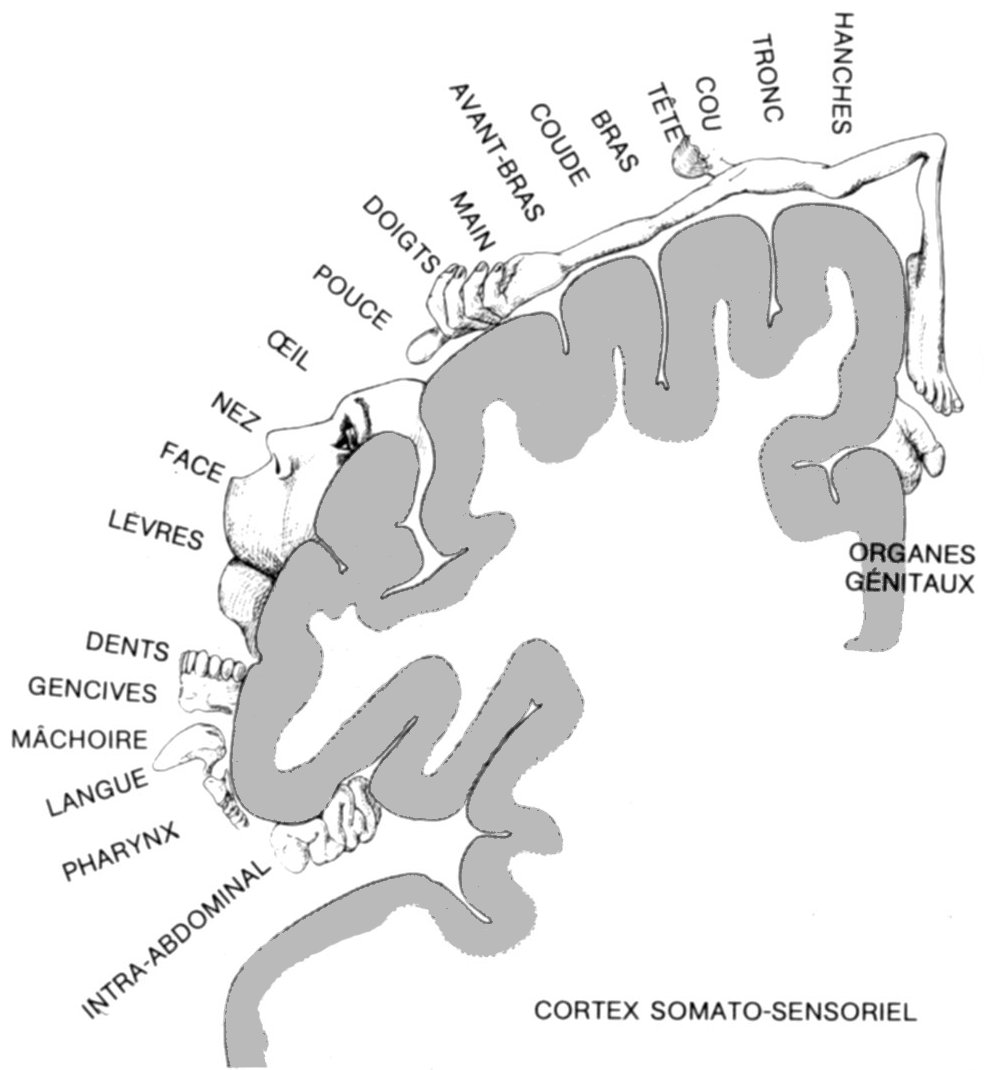
\includegraphics{img/homonculus_sensitif.png}
\caption{\label{fig:homa}Homoculi sensitifs humains~: la vue est interne
et calquée sur une coupe du cerveau~}
\end{figure}

\begin{figure}
\centering
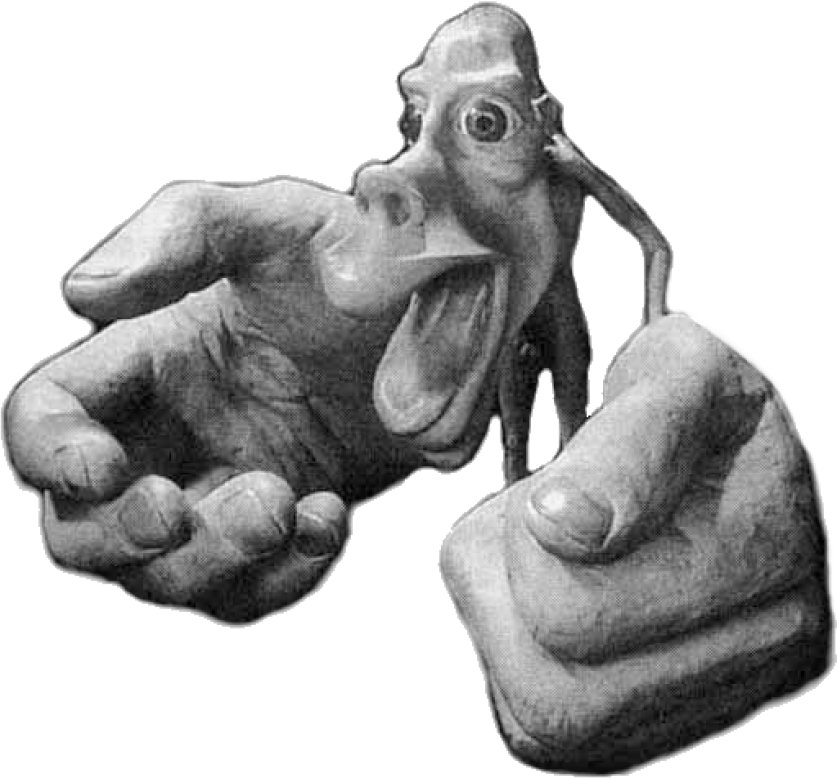
\includegraphics{img/homonculus.png}
\caption{\label{fig:homb}Homoculi sensitifs humains~: les dimensions des membres et du corps ont été
exagérées selon les capacités sensoriels de l'endroit
considéré}
\end{figure}

Historiquement, c'est grâce au compas de Weber, formé de deux pointes
sèches, qu'en 1835 il a été possible de déterminer l'acuité tactile
individuelle comme étant la plus petite distance entre deux contacts
simultanés perçus comme distincts. Les premiers homonculi ont été tracés à
cette époque. Des études plus récentes ont montré des seuils de précision sur
le sens tactile~:

\begin{itemize}
\tightlist
\item
  Discrimination entre deux points de contact avec la
  peau~: de 1 à 2,5mm.
\item
  Seuil de détection d'une force~: 63mg
\item
  Seuil de perception d'un déplacement statique~: 11,2
  µm
\end{itemize}

\hypertarget{la-perception-kinesthuxe9sique}{%
\subsection{La perception kinesthésique}\label{la-perception-kinesthuxe9sique}}

Le sens kinesthésique intègre les informations sur les positions, les
mouvements et les forces appliqués sur ou par le corps. Il est relayé par des
récepteurs situés dans les tendons musculaires au niveau des articulations,
ainsi que dans l'oreille interne. La bande passante de ces récepteurs est
plus basse que ceux de la perception tactile soit de 20 à 30 Hz. Enfin, il
s'appuie sur une utilisation de l'effet de mémoire des gestes.

La perception kinesthésique est composé par~:

\begin{itemize}
\tightlist
\item
  \textbf{Le~sens~proprioceptif}: relatif aux
  stimuli se produisant dans l'organisme. Il fournit l'information liée à la
  position du corps, et est basé sur les récepteurs situés dans les tendons
  entres les muscles et les os, dans l'oreille interne, et sur les impulsions
  du système nerveux par effet de mémoire. C'est précisément ce sens qui nous
  donne la capacité de connaître la configuration de notre corps dans
  l'espace sans avoir à le regarder.
\item
  \textbf{le sens extéroceptif}: relatif aux stimuli
  issus de phénomènes extérieurs aux corps humain. Par exemple, appréhender
  le poids, la forme ou la raideur d'un objet que l'on est en train de
  manipuler.
\end{itemize}

\textbf{Remarques~:}

\begin{enumerate}
\def\labelenumi{\arabic{enumi}.}
\tightlist
\item
  on trouve parfois dans la littérature la
  perception tactilo-proprio-kinesthésique pour désigner la perception
  haptique.
\item
  Nous considérerons par la suite, comme souvent
  dans la littérature, que le sens kinesthésique englobe le sens
  proprioceptif. En effet, d'après le Larousse, la proprioception se dit de
  la sensibilité du système nerveux aux informations sur les postures et les
  mouvements, venant des muscles et des articulations . Les trois domaines
  liés à la proprioception sont les sensibilités à la position dans l'espace,
  au mouvement du corps et aux forces exercées sur les muscles. Les deux
  premiers domaines correspondent au sens kinesthésique (\protect\hyperlink{ref-fuchs2006traite}{Fuchs, 2006}).
\end{enumerate}

\hypertarget{en-ruxe9sumuxe9}{%
\subsection{En résumé}\label{en-ruxe9sumuxe9}}

La perception des signaux spatiaux dépend de la fréquence du signal. La
distinction entre ``forme'' et ``texture'' est liée aux caractéristiques des sens
kinesthésiques et tactiles. La figure \ref{fig:Le-spectre-de} illustre la
notion de perception haptique, en terme de fréquence des stimuli.

\begin{figure}
\centering
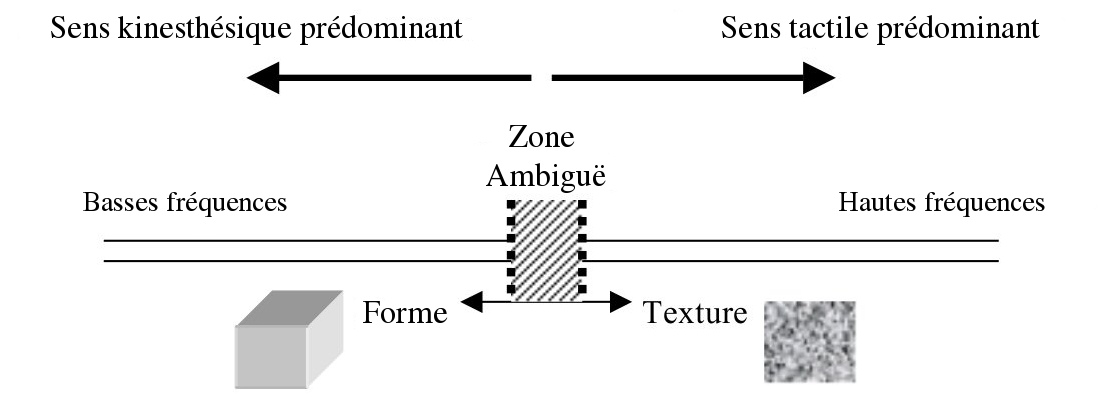
\includegraphics{img/hapticSpectrum.png}
\caption{\label{fig:Le-spectre-de}Le spectre de la perception haptique
(\protect\hyperlink{ref-wall2004investigation}{Wall, 2004})}
\end{figure}

\hypertarget{moteur}{%
\section{Le système haptique côté action~: le système moteur}\label{moteur}}

Nous allons maintenant présenter l'autre côté du système haptique tel que
nous le considérons. La partie @\ref(somesthesie) concernait le sous-système
perceptif. Ici, c'est donc le sous-système moteur qui va nous intéresser.

Et pour tenter de garder une cohérence lors de la présentation d'un
système très complexe, nous allons découper le discours en plusieurs parties,
depuis les définitions psychophysiques de bas-niveau, en remontant les
abstractions, vers les définitions de l'aboutissement de l'exécution du
système moteur~: le mouvement, puis le geste.

\hypertarget{un-petit-peu-de-psychophysique}{%
\subsection{Un petit peu de psychophysique}\label{un-petit-peu-de-psychophysique}}

Petit rappel de la définition du système haptique~: il s'agit de la
combinaison

\begin{enumerate}
\def\labelenumi{\arabic{enumi}.}
\tightlist
\item
  du système perceptif lié au toucher et à la
  kinesthésie (vu en \ref{somesthesie}),
\item
  et des mouvements d'exploration.
\end{enumerate}

Cette combinaison confère au système haptique une propriété unique~: un
même système nous permet de connaître notre environnement (sous-système
perceptif de la kinesthésie et du toucher), et d'agir sur lui (les mouvements
d'exploration).

L'objet de cette partie est de donner quelques notions sur le sens du
mouvement, lui-même lié au système moteur.

Le système moteur permet de contrôler la position du corps ainsi que les
forces à mettre en jeu lors de l'interaction avec le monde extérieur.

Pour le définir un peu plus précisément, les bandes passantes relatives au
système moteur vont suivre. La bande passante d'un système est la vitesse à
laquelle nous répondons aux stimuli par une action. Elle s'exprime en Hertz
(Hz), car nous parlons ici de fréquence~; pour obtenir le temps de réaction,
il faut prendre l'inverse.

Pour le système moteur, la bande passante oscille selon les situations
entre 1 et 10 Hz (\protect\hyperlink{ref-casiez2004contribution}{Casiez, 2004}):

\begin{itemize}
\tightlist
\item
  réponse à des signaux déstabilisant~: entre 1 et 2 Hz
  (0,5 à 1s)
\item
  réponse à des signaux périodiques~: entre 2 et 5 Hz
  (0,2 à 0,5s)
\item
  réponse à des trajectoires apprises~: 5 Hz
  (0,2s)
\item
  réponse de type réflexe~: 10 Hz (0,1s)
\end{itemize}

Pour donner un ordre d'idée sur l'intensité des forces mises en œuvre,
elles sont de l'ordre de 44N au niveau des articulations des doigts et de
102N au niveau de l'épaule pour un homme.

De manière similaire à ce que l'on a pour la perception tactile, il a été
possible de tracer un homonculus sur le système moteur humain
(figure \ref{fig:hom2}).

\begin{figure}
\centering
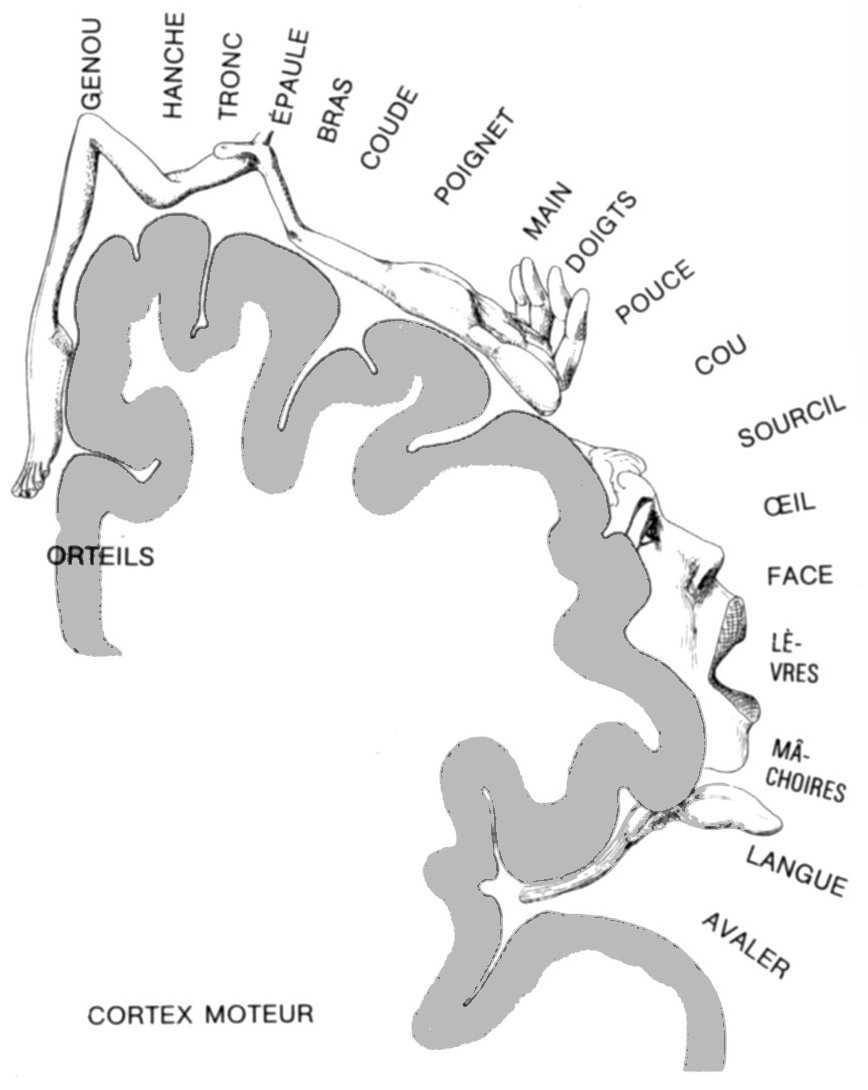
\includegraphics{img/homonculus_moteur.png}
\caption{\label{fig:hom2}Homonculus du système moteur}
\end{figure}

Toujours de manière parallèle à ce que l'on a observé pour la perception
tactile, il faudra tenir compte des capacités physiologiques du système
moteur lors de la conception de méthodes d'interaction haptique, et lors du
choix et de la position d'utilisation des périphériques.

Notre discours va à présent s'élever d'un cran, en terme d'abstraction du
système moteur~: après la psychophysique, nous abordons le concept de
mouvement, au travers de ses modélisations mathématiques.

\hypertarget{les-lois-mathuxe9matiques-liuxe9es-au-mouvement}{%
\subsection{Les lois mathématiques liées au mouvement}\label{les-lois-mathuxe9matiques-liuxe9es-au-mouvement}}

La conséquence extérieure de la mise en action du système moteur, c'est le
mouvement. Il n'est pas question ici de traiter en profondeur du mouvement,
car il faudrait une thèse entière.

Nous survolons ici quelques lois mathématiques qui tendent à modéliser le
mouvement. La loi de Fitts donne ainsi le temps nécessaire pour un geste de
pointage~; la loi d'Accot précise le temps lorsque la tâche est plus
spécifiquement un suivi de trajectoires~; la loi de puissance 2/3 et la loi de
jerk minimal tendent à modéliser les trajectoires des gestes. Enfin, le
modèle d'impulsion initiale modélise plus spécifiquement le geste de
pointage.

\hypertarget{fitts}{%
\subsubsection{La loi de Fitts}\label{fitts}}

En 1954, Fitts a empiriquement développé un prédicteur quantitatif donnant
le temps nécessaire pour effectuer une tâche de type `` acquisition et
pointage d'une cible'' (\protect\hyperlink{ref-fitts1954information}{Fitts, 1954}). Il a
présenté le rapport suivant, connu sous le nom de loi de Fitts.

Le temps du mouvement \(MT\) requis pour
sélectionner une cible de taille \(W\) situé à une
distance \(A\) est~:

\begin{equation}
 MT=a+b\log_{2}(2A/W)
 \label{eq:fitts}
\end{equation}

où \(a\) et \(b\) sont des
constantes déterminées empiriquement. Le logarithme \(\log_{2}(2A/W)\)
représente l'indice de difficulté (\(ID\)) de la
tâche et est exprimé en bits (sa base est 2). Plus élevée est la valeur de
\(ID\) et plus difficile est la tâche. Si
\(MT\) est exprimé en seconde, la constante
\(a\) sera exprimée en seconde et \(b\) en seconde/bit. L'inverse de \(b\)
(soit \(1/b\)) est l'indice de performance
(\(IP\)) et est exprimé en bit/seconde.

La figure \ref{fig:LexperiencedeFitts} illustre
l'expérience qui a permis à Fitts d'établir sa loi. La tâche que devaient
accomplir les sujets était la suivante. Initialement, la main est placée à
l'origine du mouvement~; alors, le sujet doit aller le plus vite possible
toucher une cible distante de \(A\)cm et large de
\(W\)cm.

\begin{figure}
\centering
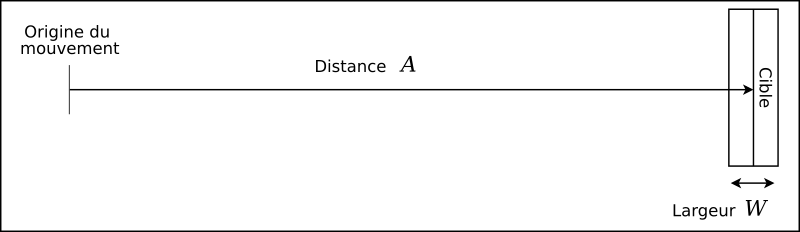
\includegraphics{img/fitts.png}
\caption{\label{fig:LexperiencedeFitts}L'expérience de Fitts}
\end{figure}

La formulation originale de la loi de Fitts \eqref{eq:fitts} s'avère
cependant inexacte pour les faibles valeur de l'\(ID\) (\textless{} 3bits), montrant une courbure de \(MT\) au dessus de la droite de régression linéaire. Une autre
formulation, proposée en 1960 par Welford (\protect\hyperlink{ref-welford1960measurement}{Welford, 1960}), permet de corriger cet
effet~:

\begin{equation}
 MT=a+b\log_{2}(A/W+0.5)
\end{equation}

Enfin, en 1992, MacKenzie (\href{047-bibliographie.html\#MacKenzie92}{MacKenzie,
1992}) a également proposé sa propre formulation~:

\begin{equation}
 MT=a+b\log_{2}(A/W+1)
 \label{eq:shannon}
\end{equation}

Ces différentes équations ne diffèrent que par la formulation de
l'\(ID\). L'équation \eqref{eq:shannon}, connue
comme formulation de Shannon, est préférée pour les raisons suivantes
(\protect\hyperlink{ref-mackenzie1992fitts}{MacKenzie, 1992})~:

\begin{itemize}
\tightlist
\item
  elle s'ajuste un peu mieux aux observations,
\item
  elle imite exactement le théorème de Shannon,
  sous-jacent à la loi du Fitts, et
\item
  elle donne toujours un nombre positif pour l'indice
  de difficulté de la tâche.
\end{itemize}

Enfin, on peut citer quelques extensions à la loi de Fitts. En effet,
cette loi ne concerne que les gestes allant d'un point à un autre en une
seule fois. Mathématiquement, on peut déduire la formulation pour un geste
effectué en deux parties (figure \ref{fig:Tachepour2}),

auxquels cas, la formulation de l'indice de difficulté \(ID\) sera~:

\[ ID\_{2}=2log_{2}\left(\frac{A}{2W}+1\right)\]

\begin{figure}
\centering
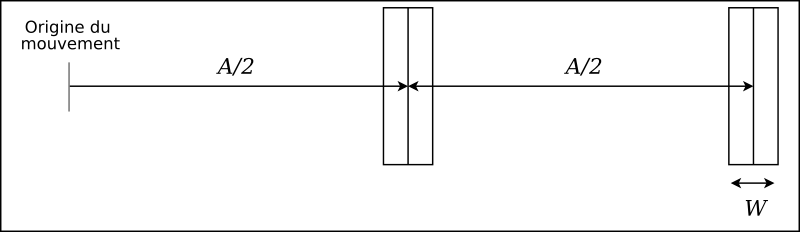
\includegraphics{img/fitts2.png}
\caption{\label{fig:Tachepour2}Tâche pour n=2}
\end{figure}

et pour n parties (figure \ref{fig:Tachepourn}):

\begin{figure}
\centering
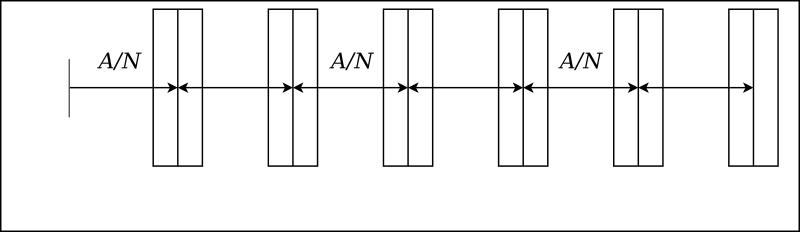
\includegraphics{img/fitts3.png}
\caption{\label{fig:Tachepourn}Tâche pour n quelconque}
\end{figure}

où on aura~:

\[ ID\_{N}=Nlog_{2}\left(\frac{A}{NW}+1\right)\]

\hypertarget{la-loi-daccot}{%
\subsubsection{La loi d'Accot}\label{la-loi-daccot}}

La loi d'Accot ou \emph{steering law} (\protect\hyperlink{ref-accot1997beyond}{Accot and Zhai, 1997}) est beaucoup plus récente, et
est utilisée pour les mouvements de suivis de chemin. L'application typique
de cette loi est l'estimation du temps de sélection d'un item dans un menu
déroulant à plusieurs niveaux (figure \ref{fig:Lecheminemprunte}).

\begin{figure}
\centering
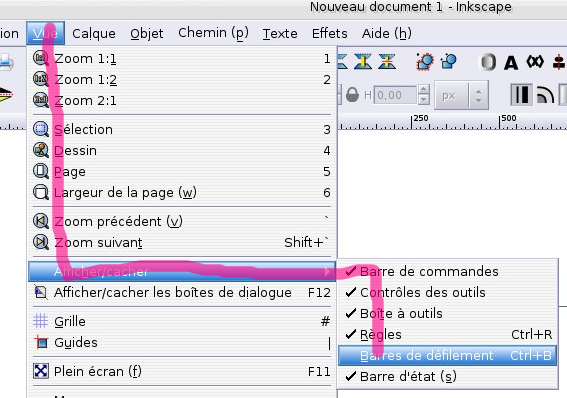
\includegraphics{img/menu_accot.png}
\caption{\label{fig:Lecheminemprunte}Le chemin emprunté pour aller chercher
un item dans des menus hiérarchiques}
\end{figure}

La loi s'exprime ainsi~:

\begin{equation}
 T\_{c}=a+b\int\_{C}\frac{ds}{W(s)}
 \label{eq:accot}
\end{equation}

où \(T\) est le temps moyen pour suivre le chemin,
\(C\) est le chemin paramétré par \(s\), \(W(s)\) est la largeur du chemin à
l'abscisse curviligne \(s\), et \(a\) et \(b\) sont des constantes empiriques.
Dans le cas général, le chemin est complexe, avec une largeur \(W(s)\) variable.

Des chemins plus simples permettent des simplifications mathématiques. Par
exemple, si le chemin est un tunnel droit avec une largeur \(W\) constante,
l'équation \eqref{eq:accot} devient~:

\[
 T=a+b\frac{A}{W}\]

où \(A\) est la longueur du chemin. On peut
observer une certaine similarité avec la loi de Fitts.

Il est également possible de dériver les deux côtés de l'équation
\eqref{eq:accot} selon la variable \(s\), et obtenir
la formulation locale, ou instantanée de la loi~:

\[
 \frac{ds}{dT}=\frac{W(s)}{b}\]

qui dit que la vitesse instantanée est proportionnelle à la largeur du
tunnel. Ceci parait logique si l'on considère l'analogie avec la conduite
d'une voiture sur une route~: plus la route est large, plus on peut
\footnote{même si l'on ne doit pas, ceci restant une expérience de pensée}
conduire vite, même s'il y a des virages.

\hypertarget{la-loi-de-puissance-23}{%
\subsubsection{La loi de puissance 2/3}\label{la-loi-de-puissance-23}}

Tout tracé curviligne peut être décomposé en parties dont chacune possède
un rayon de courbure propre et est dessinée à une certaine vitesse
tangentielle. L'analyse des mouvements d'écriture et de dessin a montré que
la vitesse augmentait dans les parties les moins courbées de la trace et
diminuait dans les parties les plus courbées. Malgré la variété de
possibilités de moduler la vitesse d'exécution d'une lettre ou d'un trait,
tous respectent une règle simple liant la vitesse tangentielle et le rayon de
courbure de la trace suivant une loi de puissance de 2/3 (\protect\hyperlink{ref-lacquaniti1983law}{Lacquaniti et al., 1983}). Cette
covariation a donné lieu à une modélisation mathématique, telle que~:

\[
 V(t)=kR(t)^{\beta}\]

où \(V\) est la vitesse tangentielle, \(R\) le rayon de courbure et \(k\) une
constante appelée gain de vitesse.

En d'autres mots, quand on tourne beaucoup, on va moins vite . On retrouve
ici la même affirmation que la loi d'Accot (voir par~:La-loi-d'Accot). Il
s'agit des mêmes phénomènes.

Il a été montré que la valeur de l'exposant β était constante et fixée à
une valeur de 1/3. La force de cette relation a été de montrer que la valeur
de cet exposant β pouvait être retrouvée dans des conditions variées
d'exécution (par exemple, différentes amplitudes du mouvement~; voir (\protect\hyperlink{ref-viviani1995minimum}{Viviani and Flash, 1995})). Ces auteurs ont alors
postulé que cet invariant reflétait la planification et la programmation du
mouvement en référence à une représentation

\hypertarget{jerk}{%
\subsubsection{Loi de jerk minimal}\label{jerk}}

Connaissant le point de départ d'un geste, le point d'arrivée, et la durée
du geste, quelle est l'équation du geste ? Comment s'assurer que ce geste
minimisera les efforts déployés (au moins au niveau de la trajectoire, de
l'évolution de la vitesse) ?

La loi de jerk minimal a été proposée par (\protect\hyperlink{ref-flash1985coordination}{Flash and Hogan, 1985}). Elle tend à exprimer
mathématiquement la trajectoire de la main (ou de tout autre extrémité du
corps) la plus douce possible.

Pour ce faire, les auteurs ont montré que la douceur d'une trajectoire
pouvait d'exprimer en fonction du jerk, c'est à dire la dérivée de
l'accélération, ou encore la dérivée 3ème de la
position.

Si on note \(x(T)\) la
position d'un système, alors le jerk de ce système sera~:

\[
 \dddot{x}(t)=\frac{d^{3}x(t)}{dt^{3}}\]

La trajectoire optimale (au sens de la douceur ) doit alors minimiser le
carré du jerk tout au long de la trajectoire. Mathématiquement, il s'agit de
minimiser la grandeur~:

\[
 H(x(t))=\frac{1}{2}\int\_{t=0}^{T}\dddot{x}^{2}dt\]

où \(T\) est la durée de la trajectoire.

Après un calcul de variation, il s'ensuit que la trajectoire minimisant le
jerk et allant d'un point \(x_i\) à un point \(x_f\) en \(d\) secondes aura pour
équation~:

\begin{equation}
 x(t)=x\_{i}+\left(x\_{f}-x\_{i}\right)\left(10\left(\frac{t}{d}\right)^{3}-15\left(\frac{t}{d}\right)^{4}+6\left(\frac{t}{d}\right)^{5}\right)
 \label{eq:jerk}
\end{equation}

Par exemple, la trajectoire pour une geste de 10cm durant 0,5sec
sera~:

\[ x(t)=800t³-2400t^{4}+1920t^{5},\quad0\leq t\leq0,5sec\]

La figure \ref{fig:Positionvitesseacceleration}
trace cette fonction, ainsi que ses trois premières dérivées~: vitesse,
accélération et jerk. La forme en cloche de la courbe de la vitesse
ẋ(\(T\)) est typique du principe de minimisation du
jerk.

\begin{figure}
\centering
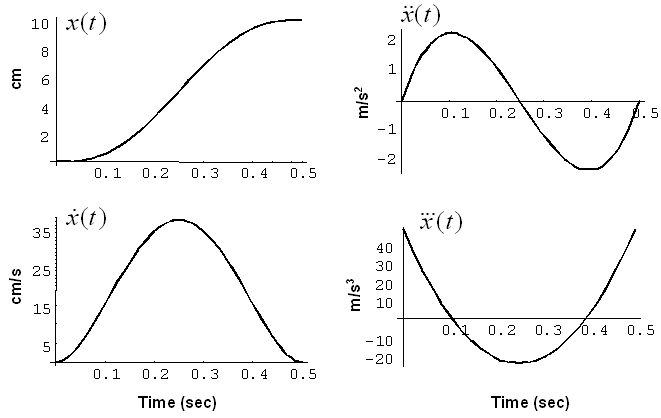
\includegraphics{img/minimu2.png}
\caption{\label{fig:Positionvitesseacceleration}Position, vitesse,
accélération et jerk de la trajectoire minimisant le jerk pour un
geste de 10cm en 0,5sec}
\end{figure}

(\protect\hyperlink{ref-flash1985coordination}{Flash and Hogan, 1985}) ont prouvé qu'en
deux dimensions ou plus, l'équation \eqref{eq:jerk} décrivait la trajectoire
assurant le jerk minimum pour chaque dimension. Par exemple, pour un
mouvement en deux dimensions, la fonction à minimiser sera~:

\[
 H\left(\underline{x}(t)\right)=\frac{1}{2}\int\_{t=0}^{T}\left(\dddot{x}^{2}+\dddot{y}^{2}\right)dt\]

et la trajectoire en deux dimensions aura pour
équation~:

\begin{equation} \underline{x}(t)=\left[\begin{array}{cc} x(t)
 &
 =x\_{i}+\left(x\_{f}-x\_{i}\right)\left(10\left(\frac{t}{d}\right)^{3}-15\left(\frac{t}{d}\right)^{4}+6\left(\frac{t}{d}\right)^{5}\right)\\
 y(t) &
 =y\_{i}+\left(y\_{f}-y\_{i}\right)\left(10\left(\frac{t}{d}\right)^{3}-15\left(\frac{t}{d}\right)^{4}+6\left(\frac{t}{d}\right)^{5}\right)\end{array}\right]
 \label{eq:jerk2}
\end{equation}

L'équation \eqref{eq:jerk2} implique qu'une trajectoire minimisant le jerk
en deux dimensions sera toujours un segment de droite.

\hypertarget{le-moduxe8le-dimpulsion-initiale}{%
\subsubsection{Le modèle d'impulsion initiale}\label{le-moduxe8le-dimpulsion-initiale}}

Le modèle le plus satisfaisant quant à la modélisation des gestes, et
notamment les gestes de pointages, a été proposé par (\protect\hyperlink{ref-meyer1988optimality}{Meyer et al., 1988}). C'est le modèle
d'impulsion initiale. D'une manière algorithmique, le processus d'une tâche
d'acquisition s'exprime ainsi~:

\begin{enumerate}
\def\labelenumi{\arabic{enumi}.}
\tightlist
\item
  Un mouvement initial est effectué pour atteindre
  la cible~;
\item
  Tant que le mouvement n'atteint pas la cible,
  faire

  \begin{enumerate}
  \def\labelenumii{\arabic{enumii}.}
  \tightlist
  \item
    refaire un mouvement pour atteindre la
    cible
  \end{enumerate}
\end{enumerate}

Le processus continue jusqu'à ce que la cible soit atteinte. L'objectif de
la tâche étant d'atteindre la cible le plus vite possible, dans le cas idéal,
le sujet touche la cible en un seul mouvement. Dans la réalité, cependant, la
précision d'un tel geste sera très faible.

\begin{figure}
\centering
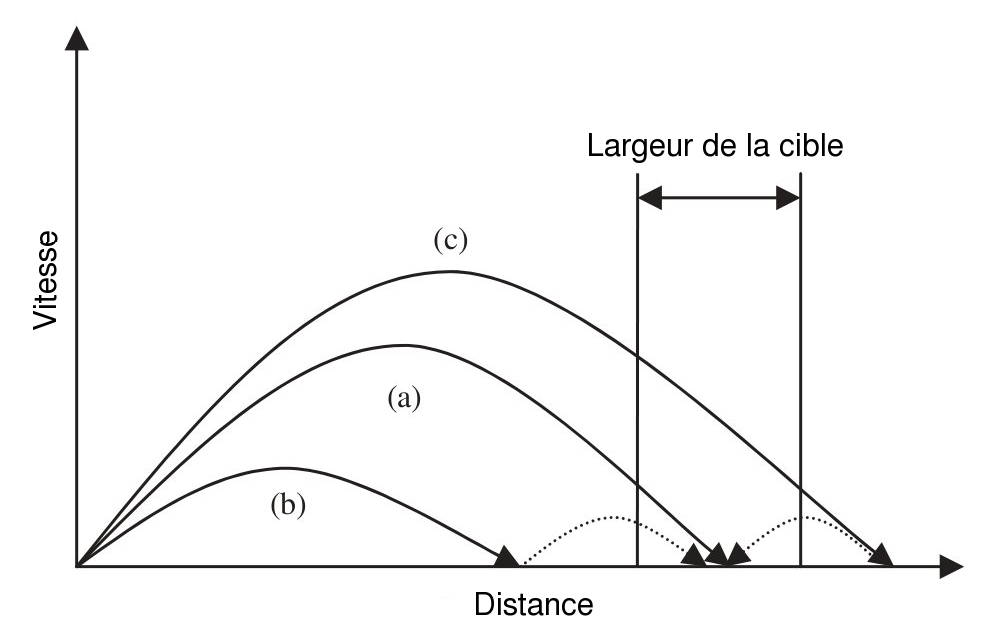
\includegraphics{img/meyer.png}
\caption{\label{fig:impulsion}Modèle d'impulsion
initiale optimisée (\protect\hyperlink{ref-meyer1988optimality}{Meyer et al., 1988})}
\end{figure}

Il a été montré (\protect\hyperlink{ref-meyer1988optimality}{Meyer et al., 1988}) (\protect\hyperlink{ref-rosenbaum1991optimal}{Rosenbaum et al., 1991}) que la
déviation standard \(s\) entre la fin du premier
mouvement et la cible augmentait avec la distance \(D\) et diminuait avec la
durée du mouvement \(T\), selon la loi~:

\[ S=k\left(\frac{D}{T}\right)\]

où \(k\) est une constante.

Ceci signifie qu'un mouvement sur une longue distance, exécuté pendant un
court laps de temps, est possible, mais aura une déviation standard élevée,
soit une faible probabilité d'atteindre la cible. De manière similaire, une
série de petits mouvements lents atteindrait très certainement la cible, mais
le temps total serait extrêmement long.

La solution mathématique au problème consiste à jouer sur \(D\) et \(T\) de manière
à minimiser le temps total (\protect\hyperlink{ref-rosenbaum1991optimal}{Rosenbaum et al., 1991}). Dans
les faits, le mouvement optimal consiste en un premier mouvement de grande
amplitude et rapide, qui nous amène aussi proche que raisonnablement possible
de la cible~; suivi par un ou plusieurs petits gestes correctifs, et plus
lents, qui se trouvent être dans les possibilités du système de contrôle
moteur.

Nous en terminons ici pour les aspects mathématiques du mouvement, et nous
allons reprendre notre ascension des niveaux d'abstraction du système moteur
: nous allons parler des gestes.

\hypertarget{duxe9finitions}{%
\subsection{Le geste~: définitions}\label{duxe9finitions}}

\begin{quote}
\textbf{Geste~:}Mouvement du corps
(principalement des mains, des bras et de la tête) volontaires
ou non, révélant un état psychologique, ou visant à exécuter
quelque chose.
Le Petit Robert - 2001
\end{quote}

L'ACROE (Association pour la Création et la Recherche sur les Outils
d'Expression) s'est intéressée au geste en le segmentant de la manière
suivante~:

\begin{enumerate}
\def\labelenumi{\arabic{enumi}.}
\tightlist
\item
  Caractérisation quantitative de l'activité
  gestuelle~:
\end{enumerate}

\textbf{Geste~digital~(Poignet~fixe)~:}
c'est le geste du sculpteur, du pianiste, du
violoniste, du dentiste. Il se caractérise par de petits déplacements
(3 cm), des précisions élevées (2 mm, 10 mN), des forces élevées (80
N)~;

\textbf{Geste~de~transport~local~(Coude~fixe)~:}
c'est le geste de positionnement de
proximité par déplacement de l'avant bras sur environ 30 cm avec des
précisions en force et en position assez faibles (0,5 cm, 10 N)~;

\textbf{Geste~de~déplacement~large~(Épaule~fixe,~ou~hanche~fixe~ou~libre)~:}
c'est un geste d'approche de faible
précision (5 cm, 100 N) par déplacement du bras ou du corps à partir de
60 cm.
2. Caractérisation qualitative et fonctionnelle de
l'activité gestuelle (\protect\hyperlink{ref-cadoz1994realites}{Cadoz, 1994}):

\textbf{une~fonction~épistémique~:}
le geste sert à connaître (un matériau, une
surface, \ldots) et est relative au retour tactile ou haptique (activation
du sens tactilo-kinesthésique)~;

\textbf{une~fonction~ergotique~:}
le geste sert à déplacer, modifier,
construire des objets matériels~; Le geste est lié à la manipulation
directe du monde physique~;

\textbf{une~fonction~sémiotique~:}
le geste sert à faire connaître~: désigner,
communiquer~; le geste véhicule une information (qui peut résulter de
l'expérience culturelle).

La fonction sémiotique du geste a vu ses caractéristiques précisée par
McNeill (\protect\hyperlink{ref-McNeill92}{McNeill, 1992}). Ainsi, un geste
sémiotique peut être~:

\textbf{Iconique~:}
le geste est parallèle à un discours
concret~;

\textbf{Métaphorique~:}
le geste est parallèle à un discours
abstrait~;

\textbf{Déictique~:}
c'est un geste de pointage ou de sélection~; ces
gestes ont reçu beaucoup d'attention car ils correspondent aux principales
tâches sur les systèmes interactifs actuels.

\textbf{bâton~:}
le geste est un battement rythmique.

\begin{quote}
Dans cette thèse, nous nous intéressons à la
fonction épistémique de l'activité gestuelle, ainsi qu'à la fonction
déictique. En effet, la première est relative au retour haptique, et la
deuxième aux gestes de pointage.
\end{quote}

\hypertarget{conjuguent}{%
\section{L'exploration haptique~: quand l'action et la perception se conjuguent sur le canal haptique}\label{conjuguent}}

Dans cette
partie, nous allons nous intéresser à la fusion des capacités de perception
\textbf{et} d'action du système haptique. Dans la littérature, il est alors
souvent question d'exploration haptique, ou encore de processus
exploratoires.

\hypertarget{guxe9nuxe9ralituxe9s}{%
\subsection{Généralités}\label{guxe9nuxe9ralituxe9s}}

Le processus d'exploration haptique met en œuvre plusieurs sous-processus
distincts.

\textbf{Petit~exemple~:}
pour déterminer la dureté d'un objet, nous
pouvons appliquer une force normale à sa surface, ou bien malaxer l'objet
dans la paume de la main si sa taille le permet. Une telle procédure
provoquerait un flux d'informations supplémentaires, concernant la
température, les capacités de conduction calorifique de l'objet, ainsi que
la texture en surface de l'objet, précisément là ou la pression a été
effectuée. De plus, si l'information obtenue est jugée insuffisante (pour
la reconnaissance de l'objet, ou bien pour l'accomplissement d'une tâche),
d'autres processus d'exploration peuvent être lancés.

Les sous systèmes concernés par une tâche d'exploration haptique sont~:

\begin{itemize}
\tightlist
\item
  le système cognitif,
\item
  les fonctions de prise de décisions,
\item
  le système moteur,
\item
  et les sensations psychophysiques issues de
  l'interaction avec les objets.
\end{itemize}

(\protect\hyperlink{ref-loomis1986tactual}{Loomis and Lederman, 1986}) et (\protect\hyperlink{ref-lederman1987haptic}{Lederman et al., 1987}) ont proposé que le
système haptique pourrait être composée de deux sous systèmes. Le système
sensoriel, et le système moteur. Selon leur interprétation, le système moteur
sert à augmenter les performances du système sensoriel, en optimisant
l'efficacité de l'exploration haptique des objets. Dans cette vision des
phénomènes, il est possible de concevoir le processus haptique comme la mise
en œuvre de fonctions haptiques de haut niveau (fonctions cognitives), et de
fonctions haptiques de bas niveau (fonctions psychophysiques). Les fonctions
haptiques de haut niveau seraient amenées à diriger les fonctions haptiques
de bas niveau~; mais pas uniquement.

\textbf{exemple~:}
si l'on décide d'aller extraire une information
de surface d'un objet, cela aura pour conséquences l'exécution d'une
procédure exploratoire (optimale pour cette information), qui se
manifestera par une série de mouvements de la main. L'interaction entre la
surface de l'objet et la peau lancera la stimulation des sens haptiques,
provoquant la perception de l'information recherchée, et par conséquent, un
modèle mental concernant la nature la surface de l'objet, se forme.

Une telle opération de haut en bas se produit quand un observateur est
dirigé vers la recherche d'une information particulière d'un objet.
Cependant, l'exploration haptique peut être dirigée de bas en haut . Dans
l'exemple précédent, et suivant les informations perceptuelles induites par
l'exploration, l'opérateur peut être conduit à explorer plus loin pour
trouver d'autres informations, qu'il ne cherchait pas nécessairement au
départ.

Ainsi, la stimulation des mécanorécepteurs provoque une réponse neurale
qui dicte l'exploration suivante. C'est la boucle comportementale (\protect\hyperlink{ref-taylor1973tactual}{Taylor et al., 1973}).

La figure \ref{fig:actionHaptique} illustre les boucles
de rétroaction se produisant lors de l'exploration haptique. Dans la
littérature, l'ensemble de ses boucles, ramené à la dualité de fonctionnement
du système (de haut en bas / de bas en haut ) a mené aux notions du contact
actif et passif . Ainsi, pendant le contact actif, un opérateur exécute
l'exploration haptique sans contrainte, déplaçant la main en contact avec un
objet. Réciproquement, pendant le contact passif, la main de l'explorateur
demeure stationnaire, alors que l'objet est déplacé en contact avec la
peau.

\begin{figure}
\centering
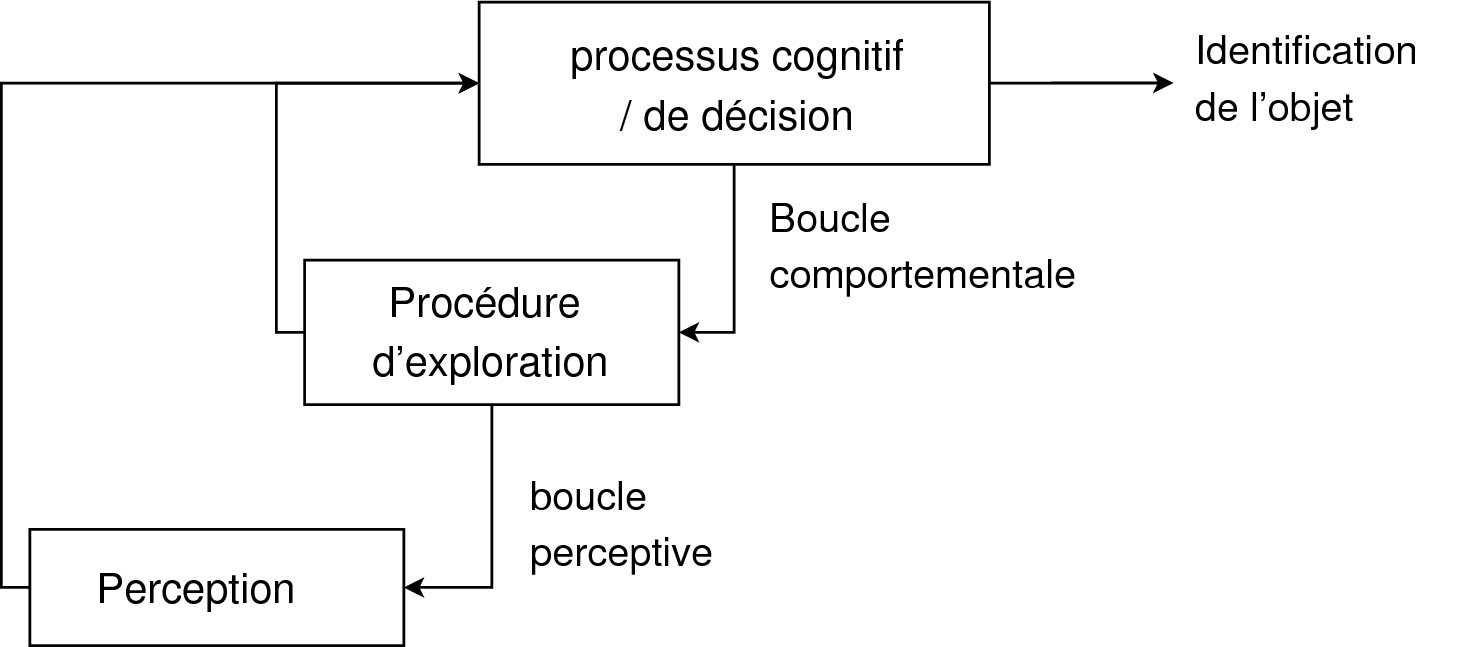
\includegraphics{img/bouclesPerception.png}
\caption{\label{fig:actionHaptique}Schéma de la perception/action haptique
(d'après (\protect\hyperlink{ref-wall2004investigation}{Wall, 2004}))}
\end{figure}

Initialement, ces concepts étaient mutuellement exclusifs (Gibson, 1962).
Pourtant, (\protect\hyperlink{ref-lederman1972fingertip}{Lederman and Taylor, 1972})
ont proposé que les concepts d'actif et de passif ne constituaient pas
nécessairement une dichotomie, mais que le processus de contact pourrait être
considéré comme ayant un certain degré de passivité . Ce degré dépendrait du
niveau de contrôle qu'a l'opérateur sur le processus de contact.

Pour terminer, (\protect\hyperlink{ref-faineteau2003kinaesthetic}{Faineteau et al., 2003}) ont mené des expériences quant à la perception des distances avec
le sens haptique. Les résultats de ces expériences peuvent se résumer de la
manière suivante~:

\begin{enumerate}
\def\labelenumi{\arabic{enumi}.}
\tightlist
\item
  Les courtes distances sont généralement
  sur-estimées, et les longues distances sont sous-estimées.
\item
  La mémoire des distances est plus volatile que la
  mémoire des positions.
\item
  La reproduction d'un mouvement actif, en terme de
  distance et de position, est plus exacte que pour un mouvement passif
  (c'est à dire aidé par un dispositif).
\end{enumerate}

\hypertarget{de-lutilisation-doutils}{%
\subsection{De l'utilisation d'outils}\label{de-lutilisation-doutils}}

L'outil est très souvent le lien entre l'humain et la tâche.

On peut citer quelques exemples du triplet Opérateur-Outil-Tâche pour les
métiers~:

\begin{itemize}
\tightlist
\item
  Le couturier - l'aiguille - la couture,
\item
  le chirurgien - le scalpel - l'incision,
\item
  ou encore, le chirurgien - le forceps
  laparoscopique, la laparoscopie\ldots{}
\end{itemize}

et d'autres exemples pour des tâches à base technologiques. On oublie ici
la spécificité de l'opérateur~: on obtient des couples Outil-Tâche~:

\begin{itemize}
\tightlist
\item
  Tournevis - Vis,
\item
  Ciseaux - Découper\ldots{}
\end{itemize}

(\protect\hyperlink{ref-dennerlein2000force}{Dennerlein et al., 2000}) ont proposé
une taxonomie des prises d'outils avec la main, selon deux axes
(figure \ref{fig:differentesgeo}).

\begin{figure}
\centering
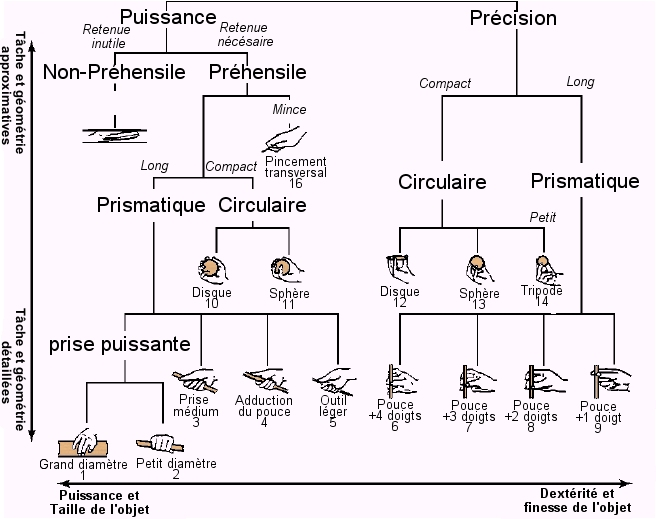
\includegraphics{img/manipulation.png}
\caption{\label{fig:differentesgeo}Les différentes géométries des prises de la
main}
\end{figure}

Les implications psychologiques de l'utilisation d'outils sur les
processus d'exploration haptique à l'aide d'outils (le contact à distance ou
\emph{remote} \emph{contact}) ont récemment été le centre de beaucoup
d'intérêt. En effet, il semble qu'il y ait équivalence entre les sensations
produites lors de l'utilisation d'un outil, et \href{017-les-applications-du-retour-haptique.html\#toc23}{celles ressenties à l'aide de
dispositifs à retour de force}.

\hypertarget{les-mouvements}{%
\subsection{Les mouvements}\label{les-mouvements}}

d'exploration

(\protect\hyperlink{ref-lederman1987haptic}{Lederman et al., 1987}) ont
identifié les différents modèles des mouvements d'exploration haptique. Dans
la liste qui suit, sont indiqués entre parenthèse les propriétés associées à
chaque mouvement d'exploration~:

\textbf{Le~mouvement~latéral~(textures)~:}
Typiquement, les doigts frottent dans les deux
sens une petite zone. Des surfaces intérieures sont explorées, plutôt que
des bordures.

\textbf{La~pression~(conformité)~:}
Une force ou un couple est appliqué à l'objet,
ce dernier étant stabilisé.

\textbf{Le~contact~statique~(température,~étirements)~:}
L'objet est soutenu, tandis qu'une main se
repose passivement sur lui.

\textbf{Le~maintient~(poids)~:}
L'objet est soulevé et maintenu dans la main,
sans chercher à le serrer. Il s'agit typiquement d'un effort du bras ou du
poignet.

\textbf{L'enveloppement~(forme,~volume~global)~:}
La main assure le plus de contacts possibles
avec l'objet. Les doigts, la paume sont mis à contribution.

\textbf{Le~suivi~de~contours~(forme,~volume~exact)~:}
Le mouvement est continu et non-répétitif sur un
bord de l'objet. Une main peut maintenir l'objet en place.

Les résultats expérimentaux ont indiqué que dans une tâche libre
d'exploration, le mouvement de la main dépendait de la caractéristique
recherchée.

\hypertarget{conclusion}{%
\section{Conclusion}\label{conclusion}}

Il s'agissait, dans ce chapitre, de se familiariser avec la très riche
terminologie liée au geste et à la perception haptique.

Nous avons également relevé quelques propriétés psychophysiques qui nous
intéresseront par la suite, comme le fait que nous ayons une meilleure
mémoire des positions et une meilleure reproduction d'un mouvement actif. Il
nous apparaît également important de souligner la dualité du système haptique
: nous avons un système perpétuel (l'information va du monde extérieur vers
nous) intimement lié au système moteur (l'information part de nous, et va
vers l'extérieur).

Dans le chapitre suivant, le monde extérieur sera une machine ou un
ordinateur~: on parle alors d'interaction homme-machine, ou de communications
homme-machine.

\hypertarget{communications-homme-machine}{%
\chapter{Communications Homme-Machine}\label{communications-homme-machine}}

\hypertarget{introduction-2}{%
\section{Introduction}\label{introduction-2}}

Maintenant que nous avons passé en revue les définitions et concepts
propres à l'humain, en matière de perceptions et d'actions basées sur les
sensations haptiques, nous allons étendre dans ce chapitre, notre étude à la
machine~: nous allons donc glisser vers le domaine de l'interaction
Homme-Machine, ou IHM.

Pour commencer, seront posées les principales définitions du domaine de
l'IHM. La section suivante présentera les modélisations de l'utilisateur,
dans un système interactif. Dans les deux parties suivantes, nous
présenterons les moyens techniques d'interaction, basée sur la sensation
haptique, d'abord dans le sens humain-machine (en entrée du système), puis
dans le sens machine-humain (en sortie, donc).

Nous terminerons ce chapitre en présentant l'intégration du mode haptique
au sein des systèmes interactifs, puis les applications existantes, mettant
en œuvre cette interaction haptique.

\hypertarget{les-systuxe8mes-interactifs}{%
\section{les systèmes interactifs}\label{les-systuxe8mes-interactifs}}

Un système interactif est une application informatique qui prend en
compte, au cours de son exécution, d'informations communiquées par le ou les
utilisateurs du système, et qui produit, au cours de son exécution, une
représentation perceptible de son état interne (\protect\hyperlink{ref-beaudouin1997ingenierie}{Beaudouin-Lafon, 1997}).

Un système interactif est généralement composé de deux parties~:
l'interface utilisateur et le noyau fonctionnel
(\ref{fig:decompositiondunsysteme}). L'interface utilisateur est
constituée des éléments logiciels et matériels qui sont mis en œuvre lors de
la capture des entrées de l'utilisateur et lors de la restitution des sorties
du système. Le noyau fonctionnel représente le système de traitement et de
stockage de l'information.

\begin{figure}
\centering
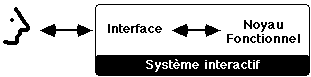
\includegraphics{img/sys_inter.png}
\caption{\label{fig:decompositiondunsysteme} Décomposition d'un système
interactif}
\end{figure}

Il est possible de modéliser un système interactif suivant plusieurs
points de vue, selon que l'on s'intéresse au domaine de l'application, à
l'architecture logicielle ou aux aspects ergonomiques et cognitifs entrant en
jeu dans l'utilisation du système. La figure \ref{fig:modelisationsdunsysteme}
reflète différentes approches que l'on peut avoir d'un système

\begin{figure}
\centering
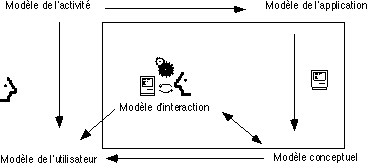
\includegraphics{img/I21.png}
\caption{\label{fig:modelisationsdunsysteme}Modélisations d'un système
informatique interactif. Les flèches indiquent les relations de
dépendance de chaque modèle (tiré de (\protect\hyperlink{ref-baudel1995aspects}{Baudel, 1995}))}
\end{figure}

Chacun des modèles présentés correspond à une vue que peut se former un
observateur en fonction de son rôle dans l'élaboration.

\begin{itemize}
\tightlist
\item
  Le commanditaire du système est principalement
  préoccupé par l'activité (ou la tâche) que le système aidera à
  effectuer.
\item
  Le concepteur de l'application a pour objectif de
  spécifier un système logiciel correspondant au modèle de l'activité.
\item
  Le concepteur de l'interface propose une
  représentation des objets et des méthodes d'interaction efficaces et
  compréhensibles pour l'utilisateur, en fonction de l'application (modèle
  conceptuel) et du système informatique utilisé (modèle d'interaction).
\item
  Enfin, l'utilisateur utilise un système en fonction
  de ses connaissances du domaine (activité) et du système (modèle
  d'interaction et modèle conceptuel de l'application).
\end{itemize}

Posons maintenant la terminologie de ce domaine.

\hypertarget{linteraction-et-linterface-homme-machine}{%
\subsection{L'Interaction et l'Interface Homme-Machine}\label{linteraction-et-linterface-homme-machine}}

L'interaction homme-machine désigne l'ensemble des phénomènes physiques et
cognitifs qui interviennent dans la réalisation de tâches avec le concours de
l'ordinateur.

L'interface homme-machine désigne un assemblage de composants logiciels et
matériels qui permet l'accomplissement de tâches avec le concours de
l'ordinateur.

Les composantes de l'interaction homme-machine sont~:

\begin{enumerate}
\def\labelenumi{\arabic{enumi}.}
\tightlist
\item
  L'utilisateur
\item
  accomplit une tâche
\item
  dans un contexte particulier
\item
  en utilisant un système informatique.
\end{enumerate}

\hypertarget{quelques-duxe9finitions-de-la-communication-multimodale}{%
\subsection{Quelques définitions de la communication multimodale}\label{quelques-duxe9finitions-de-la-communication-multimodale}}

Les définitions qui font référence sont le fait de (\protect\hyperlink{ref-coutaz1991taxonomy}{Coutaz and Caelen, 1991}).

\textbf{Mode de communication~:}
D'après le petit robert, un mode est une norme
particulière sous laquelle se présente un fait, s'accomplit une action. En
grammaire, le mode est un trait dénotant la manière dont le locuteur
présente le procès (on dit plus couramment action). Du point de vue
système, un mode représente l'état dans lequel le système s e trouve à un
moment donné. Un mode fait référence aux cinq sens de l'être humain~: le
toucher, l'ouïe, la vue, l'odorat, le goût (réception d'information), et
aux différents moyens d'expression humains~: le geste, la parole (émission
d'information). Il définit la nature des informations servant pour la
communication (mode visuel, mode sonore, mode gestuel etc.).

\textbf{Modalités~:}
Une modalité est une forme concrète particulière
d'un mode de communication. Par exemple, le bruit, la musique, la parole
sont des modalités du mode sonore.

\textbf{Média~:}
Dans la vie courante, un média désigne un
support d'information (journal, disque audio\ldots). En informatique, un média
peut également être un support (vidéodisque, CD-ROM\ldots), mais actuellement,
par extension, il désigne le dispositif physique qui acquiert ou qui
diffuse l'information~: un écran vidéo, un système de synthèse de parole\ldots{}
Dans un sens large, les médias désignent les différents périphériques
d'ordinateur (plutôt non conventionnels) qui permettent la communication,
en entrée comme en sortie.

\textbf{Communication multimodale~:}
une communication est dite multimodale si elle
fait intervenir plusieurs modes de communications dans les échanges
d'information. Cependant, en informatique, ce qualificatif s'applique
également pour les communications ne faisant intervenir qu'un seul mode
mais avec plusieurs modalités.

\textbf{Système multimodal~:}
théoriquement, un système informatique
multimodal est un système capable d'intégrer plusieurs modes de
communication. Cependant, on désigne également par ce nom tout système
capable d'intégrer plusieurs modalités de communication (même s'il
n'intègre qu'un seul mode).

\textbf{Multimodalité :}
le terme de multimodalité fait référence à
l'usage de plusieurs modalités pour la réalisation d'une même tâche.

\textbf{Multimédia~:}
un système informatique multimédia est un
système capable d'acquérir et/ou de restituer, par l'intermédiaire des
médias, des informations de natures et/ou de formes différentes (parole,
musique, image vidéo, etc.).

Ces trois notions sont dépendantes les unes des autres. En effet, à un
mode correspond un ensemble de modalités et à une modalité est rattaché un
ensemble de média permettant son expression.

\textbf{Exemple~:} La modalité «~Vibration~» s'exprime par exemple sur le
médium «~Vibreur~» et fait appel au mode Tactile .

\hypertarget{les-interfaces-informatiques-actuelles-les-interfaces-wimp}{%
\subsection{Les interfaces informatiques actuelles~: les interfaces WIMP}\label{les-interfaces-informatiques-actuelles-les-interfaces-wimp}}

Dans le champs de recherche de l'Interaction Homme-Machine (IHM),
l'acronyme WIMP signifie \emph{Windows, Icons, Menus, Pointing} pour
fenêtres, icônes, menus et pointage. Il s'agit des interfaces graphiques que
nous utilisons le plus souvent devant un ordinateur. Les interfaces WIMP ont
été imaginées et développées au Xerox PARC en 1973 et ont été popularisée
avec le Macintosh en 1984.

En anglais populaire, le terme WIMP est couramment utilisé pour insulter
les personnes qui manquent de force et/ou de courage. Cet usage était courant
avant l'arrivée des interfaces graphiques. Maintenant, il arrive que WIMP
soit utilisé d'une manière dénigrante, en particulier par les personnes qui
préfèrent les interfaces traditionnelles comme les interfaces à ligne de
commande.

On parle enfin d'interface POST-WIMP pour les interfaces qui se basent sur
d'autres paradigmes d'interaction (\href{047-bibliographie.html\#Dam1997}{van Dam,
1997}).

\hypertarget{les-moduxe8les-de-lutilisateur}{%
\section{Les modèles de l'utilisateur}\label{les-moduxe8les-de-lutilisateur}}

\hypertarget{processeur}{%
\subsection{Le modèle du processeur humain et les caractéristiques du corps humain}\label{processeur}}

Dans leur modèle, The Model Human Processor , S. Card, T. Moran et A.
Newell représentent l'individu comme un système de traitement d'informations
régi par des règles (\href{047-bibliographie.html\#Card1983}{Card et~al.,
1983}). Le processeur humain comprend trois sous-systèmes interdépendants
: les systèmes sensoriel, moteur et cognitif. Chacun d'eux dispose d'une
mémoire et d'un processeur dont les performances se caractérisent à l'aide de
paramètres (figure \ref{fig:processorhumain}).

Pour une mémoire, les paramètres essentiels sont~:

\begin{itemize}
\tightlist
\item
  µ (ou \emph{m}), la capacité:
  le nombre d'éléments d'information mémorisés~;
\item
  δ (ou \emph{d}), la
  persistance~: temps au bout duquel la probabilité de retrouver un élément
  d'information est inférieure à 0,5~;
\item
  κ (ou \emph{k}), le type
  d'information mémorisée (physique, symbolique, etc.).
\end{itemize}

Pour un processeur, le paramètre important est

\begin{itemize}
\tightlist
\item
  τ (ou \emph{t}), le cycle de
  base qui inclut le cycle d'accès à sa mémoire locale.
\end{itemize}

\begin{figure}
\centering
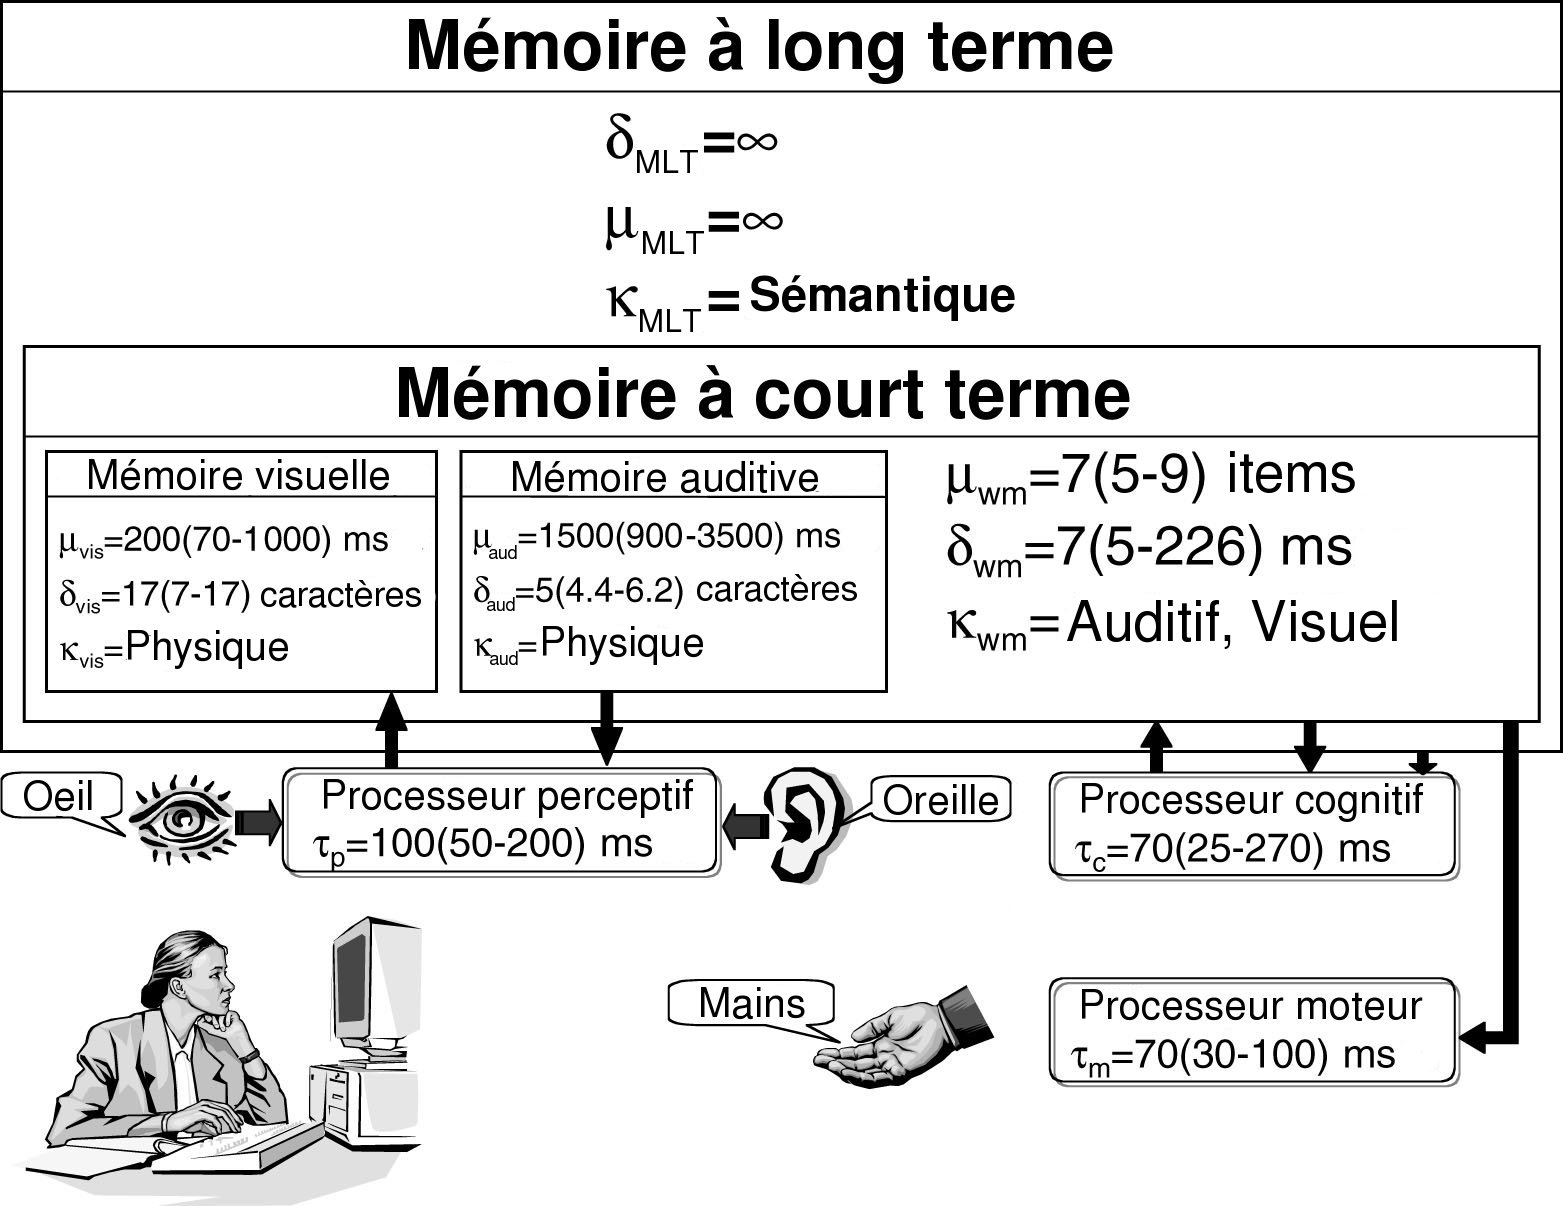
\includegraphics{img/humanProcessor.png}
\caption{\label{fig:processorhumain}Le modèle du processeur humain (d'après
(\protect\hyperlink{ref-booth2004human}{Booth, 2004}))}
\end{figure}

Ce modèle nous donne un certain nombre d'informations sur la mémoire à
court terme~:

\begin{itemize}
\tightlist
\item
  nous mémorisons 7 items (± 2 selon l'individu, la
  fatigue\ldots)~;
\item
  nous regroupons les mnèmes (ie les unités
  d'information) par motifs visuels, acoustiques, perpétuels~;
\item
  lors d'une recherche d'information, celle-ci a lieu
  de manière séquentielle~;
\item
  enfin, l'oubli de la mémoire à court terme est de
  l'ordre de 15 à 30 secondes.
\end{itemize}

Et ceci peut se retrouver dans une conception des interfaces de systèmes
interactifs~:

\begin{itemize}
\tightlist
\item
  limiter les items de menus à 7
\item
  établir des liens entre éléments (couleurs, format,
  emplacements) pour faciliter le filtrage cognitif
\item
  écrire des messages concis
\item
  ne pas présenter d'informations inutiles
\end{itemize}

\begin{figure}
\centering
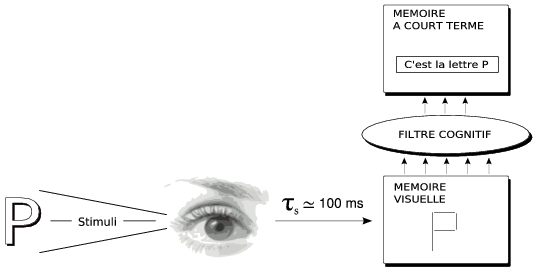
\includegraphics{img/systemecognitif.png}
\caption{\label{fig:coutaz}Le système sensoriel visuel et sa relation avec le système
cognitif (tiré et adapté de (\protect\hyperlink{ref-coutaz1988interface}{Coutaz, 1988}))}
\end{figure}

\hypertarget{par-rapport-au-systuxe8me-moteur}{%
\paragraph{Par rapport au système moteur}\label{par-rapport-au-systuxe8me-moteur}}

Outre le modèle de l'homonculus déterminé expérimentalement, le modèle du
processeur humain propose une mesure quantitative des performances motrices
humaines en fonction des organes considérés. Il est ainsi possible de
déterminer les principales zones fonctionnelles de l'être humain par ordre
d'importance et d'utilité dans l'interaction (extrait de (\protect\hyperlink{ref-baudel1995aspects}{Baudel, 1995})):

\begin{itemize}
\tightlist
\item
  \emph{la} \emph{main dominante, constituée des 5
  doigts et de la paume, présente 23 degrés de liberté (sans les poignets).
  Ces degrés ne sont bien sûr pas interdépendants. La main et les doigts sont
  les organes les plus utilisés et vraisemblablement les plus utiles à
  l'interaction.}\href{\%5BSturman,\%201992\%5D(047-bibliographie.html\#Sturman1992)}{\ldots{}}
\item
  \emph{la main non dominante, identique à la main
  dominante, mais ayant un contrôle moteur moins précis.}
\item
  \emph{les lèvres et langue, les muscles faciaux
  présentent un grand nombre de degrés de liberté utilisés de façon très
  subtile dans la communication humaine. Ces degrés de liberté sont cependant
  difficilement exploitables~: ils sont déjà utilisés pour la communication
  vocale, leur emploi est fortement stéréotypé, dépendante du milieu
  socioculturel et sont difficile à interpréter.} {[}\ldots{]}
\item
  \emph{les poignets et bras (coude): Le poignet est lié
  à la main et ne peut être utilisé indépendamment de celle-ci lorsqu'elle
  est déjà mise à contribution. Certaines machines-outils utilisent le coude
  comme moyen d'actionnement d'interrupteurs.}
\item
  \emph{les pieds~: Que ce soit en position assise ou
  debout, le pied est assez précisément contrôlable et peut être utilisé}
  {[}\ldots{]} \emph{(pédalier de l'orgue} {[}\ldots{]} \emph{contrôle du volume ou du
  vibrato sur un harmonium ou un orgue électronique, accélérateur d'une
  voiture\ldots). De nombreux outils et instruments utilisent des pédaliers et
  des pédales à course pour remédier à l'occupation des membres supérieurs
  par d'autres contrôles. De plus, le pied peut être utilisé lorsque la force
  requise pour actionner un effecteur doit être assez importante.}
\item
  \emph{les jambes~: Les jambes ne peuvent être
  facilement utilisées lorsque le pied est mis à contribution. Certaines
  machines outils utilisent cependant des interrupteurs activés par le
  genou.}
\item
  \emph{le tronc présente autant de degrés de liberté
  qu'il y a de vertèbres et de côtes, mais ces dimensions sont assurément
  difficiles à utiliser activement dans l'interaction avec un ordinateur.
  Tout au plus une mesure de l'état général de relâchement du corps peut-il
  indiquer une fatigue de l'utilisateur et une baisse de son
  attention.}
\end{itemize}

\hypertarget{autres-moduxe8les-de-lutilisateur}{%
\subsection{Autres modèles de l'utilisateur}\label{autres-moduxe8les-de-lutilisateur}}

\textbf{GOMS}
(\emph{Goal, Operator, Method, Selection})
(\protect\hyperlink{ref-card2018psychology}{Card et al., 2018}) se contente de
modéliser le comportement observable de l'utilisateur (approche
béhavioriste) et ne cherche pas à décrire les états mentaux et les
traitements internes (approche cognitiviste).
\textbf{KeyStroke}
(\href{047-bibliographie.html\#Card1983}{Card et~al.,
1983}) est une version simplifiée de GOMS. Il permet de prédire le temps
d'exécution de cette tâche par un utilisateur expert. On suppose que la
méthode est unique, on ne prend pas en compte l'opération de choix s'il y a
plusieurs méthodes candidates pour le même but.

\textbf{La~théorie~de~l'action}
(\protect\hyperlink{ref-norman1988psychology}{Norman, 1988}) est une approche cognitiviste de la modélisation de l'utilisateur
: l'individu élabore un modèle conceptuel du système informatique. Le
comportement est conditionné par l'environnement et par la représentation
interne que l'utilisateur se fait du système. La figure \ref{fig:norman} illustre ce modèle de l'action. Le point fort de
cette approche est qu'elle permet d'expliquer les réussites, difficultés et
erreurs de l'utilisateur.

\begin{figure}
\centering
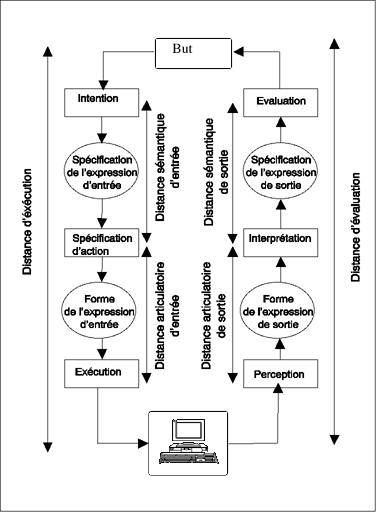
\includegraphics{img/design.png}
\caption{\label{fig:norman}Le modèle de l'action de Norman}
\end{figure}

\hypertarget{les-puxe9riphuxe9riques-dentruxe9e}{%
\section{Les périphériques d'entrée}\label{les-puxe9riphuxe9riques-dentruxe9e}}

\hypertarget{petit-point-historique}{%
\subsection{Petit point historique}\label{petit-point-historique}}

Pour manipuler un point dans l'espace virtuel de la mémoire de
l'ordinateur, nous avons besoin d'un dispositif dit de pointage. Le plus
commun de ces dispositifs, c'est la souris. La figure
\ref{fig:Lapremieresouris} montre la première souris de l'histoire,
créée par Douglas Engelbart et William English en 1964.

\begin{figure}
\centering
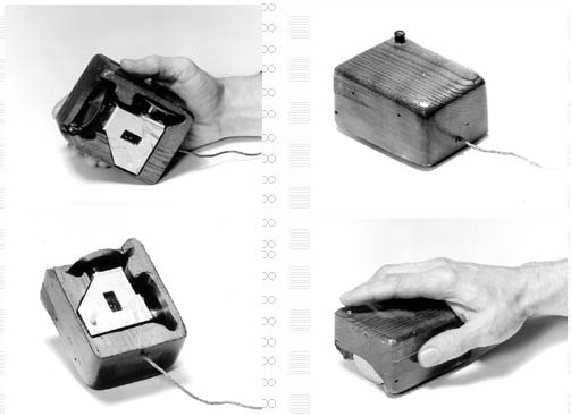
\includegraphics{img/firstMouse.png}
\caption{\label{fig:Lapremieresouris}La première souris de l'histoire}
\end{figure}

\hypertarget{taxonomie-des-puxe9riphuxe9riques-dentruxe9e}{%
\subsection{Taxonomie des périphériques d'entrée}\label{taxonomie-des-puxe9riphuxe9riques-dentruxe9e}}

\textbf{Comment classer les différents périphériques qui ont été imaginés pour
interagir avec l'ordinateur ?}

Certains périphériques sont conçus pour un mode d'utilisation reposant sur
un changement d'états discrets~: par exemple, une touche est enfoncée ou non~;
ou encore, la position d'un capteur est une valeur entière comprise entre 1
et 10. Ce sont les périphériques à états discrets. Le clavier en est
l'exemple type.

D'autres périphériques, comme la souris, sont dénommés à entrée continue.
Ils produisent un échantillonnage, ou une trace du geste réalisé pour
actionner le périphérique.

Les premières classifications des périphériques d'entrée sont le fait de
Foley, Wallace et Chan (\href{047-bibliographie.html\#Foley1984}{Foley et~al.,
1984}) et de Buxton (\protect\hyperlink{ref-buxton1983lexical}{Buxton, 1983}).
Foley et ses collègues se sont basés sur les tâches graphiques que chaque
périphérique est capable de réaliser. Buxton a classifié les périphériques
d'entrée selon leurs propriétés physiques et leur nombre de degrés de
libertés. Finalement, Card et ses collègues (\protect\hyperlink{ref-card1991morphological}{Card et al., 1991}) ont repris la
classification de Buxton et l'ont étendue à l'ensemble des périphériques à
degrés de liberté continus et discrets. Dans un premier temps, le
tableau~\protect\hyperlink{cap:Inventaire-des-grandeurs}{2.1} récapitule les
grandeurs que l'on utilise pour classer les périphériques à retour d'effort,
selon la nature des degrés de liberté.

\begin{longtable}[]{@{}llll@{}}
\toprule()
\endhead
& Degrés de liberté & & \\
Linéaire & Rotatif & & \\
Position & absolue & Position \emph{P} & angle \emph{R} \\
relative & mouvement δ \emph{P} & delta angle δ \emph{R} & \\
Force & absolue & Force \emph{F} & couple \emph{T} \\
relative & delta Force δ \emph{F} & delta couple δ \emph{T} & \\
\bottomrule()
\end{longtable}

Table 2.1~: Inventaire des grandeurs
mesurables sur un périphérique d'entrée continu en fonction de la
nature du degré de liberté

Le modèle de (\protect\hyperlink{ref-card1991morphological}{Card et al., 1991}) se
propose de placer les périphériques d'entrée dans un espace permettant de les
comparer. Le nombre de dimensions de cet espace n'est pas fixé. Tout critère
de comparaison entre deux dispositifs peut en fournir une. Les dimensions les
plus importantes sont le nombre et le type des degrés de liberté des
dispositifs d'entrée considérés. Le tableau suivant est constitué de 5
axes~:

\begin{itemize}
\tightlist
\item
  dispositif de translation ou de rotation.
\item
  dimension de l'espace (x, y, z ou lacet, tangage et
  roulis) captée.
\item
  déplacement absolu ou relatif.
\item
  capteur de mouvement ou de force.
\item
  résolution (entre 1 bit et l'infini).
\end{itemize}

La figure \ref{fig:Espacedeconception} reprend la taxonomie de
(\protect\hyperlink{ref-card1991morphological}{Card et al., 1991}), ainsi que celle de chacun de ses prédécesseurs.

\begin{figure}
\centering
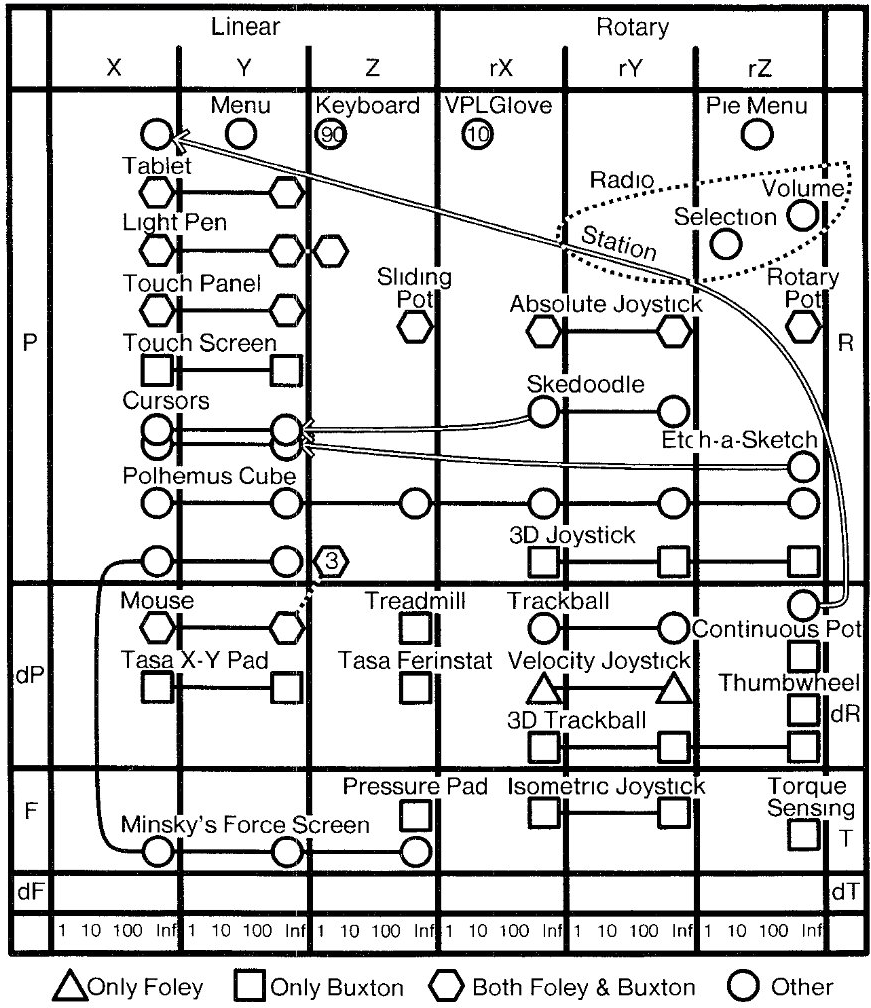
\includegraphics{img/cards.png}
\caption{\label{fig:Espacedeconception}Espace de conception des dispositifs d'entrée (tiré de
(\protect\hyperlink{ref-card1991morphological}{Card et al., 1991}))}
\end{figure}

\hypertarget{performances}{%
\subsection{Les performances en entrée des périphériques de pointage}\label{performances}}

Pour évaluer les performances des dispositifs de pointage, les recherches
ont souvent utilisé la loi de Fitts (voir \ref{fitts}). La
figure \ref{fig:accot} montre les performances de différents
dispositifs de pointage selon la loi d'Accot (voir par~:La-loi-d'Accot).

\begin{figure}
\centering
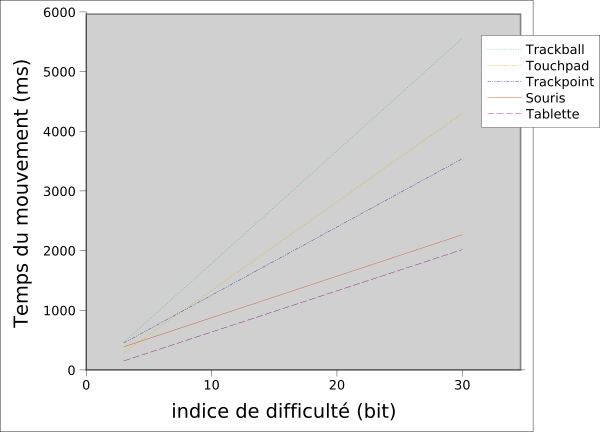
\includegraphics{img/steering.png}
\caption{\label{fig:accot}Les performances des périphériques de pointage selon la loi d'Accot (tiré
de (\protect\hyperlink{ref-accot1999performance}{Accot and Zhai, 1999}))}
\end{figure}

\hypertarget{comment-lire-ce-graphique}{%
\paragraph*{Comment lire ce graphique ?}\label{comment-lire-ce-graphique}}
\addcontentsline{toc}{paragraph}{Comment lire ce graphique ?}

L'axe horizontal indique l'indice de difficulté de la tâche. Comme il
s'agit de la loi d'Accot, l'indice de difficulté est relatif ici à la largeur
de la trajectoire à suivre, et à sa rectilinéarité (est-elle très courbée ou
non).

L'axe vertical indique le temps du mouvement (en ms).

Donc, plus le segment de droite est bas sur ce graphique, plus le
dispositif correspondant est efficace dans une tâche de suivi de
trajectoire.

La souris apparaît comme un des périphériques les plus performants, avec
la tablette graphique. Ensuite, le trackpoint (le petit joystick disponible
sur certains portables pour manipuler le pointeur), le touchpad (le petit
écran tactile des ordinateurs portables) et le trackball, sont beaucoup moins
performants.

Une autre étude (\protect\hyperlink{ref-mackenzie2001accuracy}{MacKenzie et al., 2001}) confirme ce résultat (figure \ref{fig:performances}).

\begin{figure}
\centering
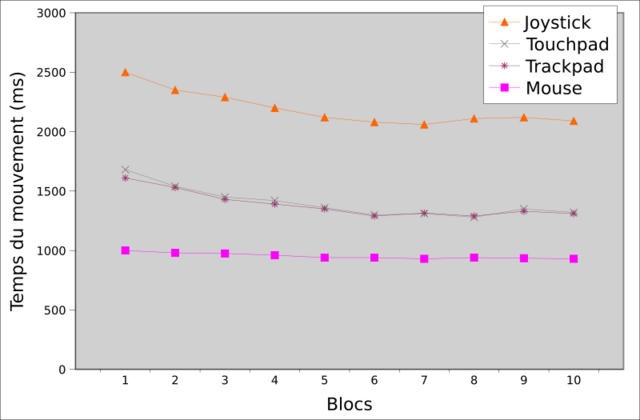
\includegraphics{img/comparaison.png}
\caption{\label{fig:performances}Les performances de dispositifs de pointage (adapté de (\protect\hyperlink{ref-mackenzie2001accuracy}{MacKenzie et al., 2001})}
\end{figure}

\hypertarget{la-tuxe2che-effectuuxe9e-et-linterpruxe9tation-de-ce-graphique}{%
\paragraph*{La tâche effectuée et l'interprétation de ce graphique}\label{la-tuxe2che-effectuuxe9e-et-linterpruxe9tation-de-ce-graphique}}
\addcontentsline{toc}{paragraph}{La tâche effectuée et l'interprétation de ce graphique}

Les sujets devaient aller pointer le plus vite possible, différentes
cibles placées sur un cercle. La figure \ref{fig:Latache} précise l'ordre des
mouvements à réaliser.

\begin{figure}
\centering
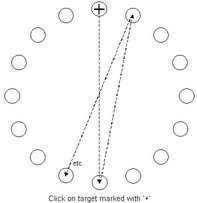
\includegraphics{img/CHI01-f6.jpg}
\caption{\label{fig:Latache}La tâche de pointage dans l'expérience de
McKenzie}
\end{figure}

Sur le graphique de la figure \ref{fig:performances}, on retrouve bien le fait
que la souris est bien plus efficace que les autres dispositifs de pointage. Il
y a également un effet d'apprentissage qui apparaît (le temps du mouvement
diminue au fur et à mesure de l'expérience), mais ce n'est pas le sujet de
notre discussion.

Enfin, d'un point de vue ergonomique, (\protect\hyperlink{ref-zhai1996influence}{Zhai et al., 1996}) a démontré que les
périphériques d'entrée manipulés avec les doigts, obtiennent de meilleures
performances lors d'une tâche de pointage, que les dispositifs qui nécessitent
la mise en action du poignet et/ou du coude et/ou de l'épaule.

\begin{quote}
Ceci doit nous amener à inciter les utilisateurs
à se placer dans une position leur intimant d'utiliser la précision de
leurs doigts, avec le bras le plus reposé possible.

\hypertarget{le-geste-dans-les-systuxe8mes-interactifs}{%
\subsection{Le geste dans les systèmes interactifs}\label{le-geste-dans-les-systuxe8mes-interactifs}}
\end{quote}

(\protect\hyperlink{ref-baudel1995aspects}{Baudel, 1995}) a relevé trois
paradigmes d'utilisation du canal haptique en entrée dans les systèmes
interactifs. Il a défini l'entrée haptique comme tout mode d'interaction
faisant intervenir les divers modes d'action liés aux sens haptiques . Ce que
nous pouvons considérer comme le geste vers la machine .

\hypertarget{entruxe9e-haptique-simple}{%
\subsubsection{Entrée haptique simple}\label{entruxe9e-haptique-simple}}

(\protect\hyperlink{ref-baudel1995aspects}{Baudel, 1995}) parle d'entrée haptique
simple lorsque la sémantique d'une action est entièrement décrite par des
changements d'état discrets du dispositif.

Par exemple, pour tracer un rectangle avec une souris, le bouton enfoncé
fournit une première position d'ancrage, le relâchement une deuxième. Ces
deux positions suffisent à elles seules à fournir les paramètres de création
du rectangle~; la façon avec laquelle l'utilisateur déplace la souris n'a pas
d'incidence sur la signification engendrée par le geste.

\hypertarget{reconnaissance-de-marques-et-de-tracuxe9s}{%
\subsubsection{Reconnaissance de marques et de tracés}\label{reconnaissance-de-marques-et-de-tracuxe9s}}

On appelle reconnaissance de marques et de tracés, la prise en compte de
la trajectoire réalisée avec le dispositif de pointage.

Dans l'exemple du rectangle, on peut imaginer une autre façon de faire~:
avec la souris, on peut tracer directement les 4 côtés du rectangle. Le
système se chargera de paralléliser les tracés forcément approximatifs, en
fonction de ce qu'il a reconnu.

Cette technique possède un autre avantage~: il n'y a plus de déclaration
d'intention. Dans notre exemple, il n'est plus nécessaire de choisir l'outil
dessine un rectangle puis de le tracer~; on peut dessiner directement.

La reconnaissance de marques, ou de tracés, permet d'enrichir la
sémantique des actions élémentaires de l'utilisateur.

Ce type d'interaction est déjà utilisé dans quelques applications. Par
exemple, le navigateur internet Opera, dispose d'une reconnaissance de
marques. Par exemple, un geste avec la souris vers la gauche, tout en
maintenant le bouton du milieu enfoncé, rechargera la page précédente.

Dans un éditeur d'objets en deux dimensions, (\protect\hyperlink{ref-kurtenbach1991issues}{Kurtenbach and Buxton, 1991}) ont utilisé
toute une variété de gestes qui simplifiaient la sélection, l'effacement, le
déplacement ou la duplication d'un objet ou d'un groupe d'objets. La
figure \ref{fig:gestes1} présente ces gestes. Par
exemple, effacer un objet est réalisé en barrant cet objet (a)~; effacer un
groupe d'objets consiste en dessinant une zone autour de ces objets puis en
terminant le tracé à l'intérieur de cette zone (b) ~; le déplacement d'objets
commence comme l'effacement de groupe, mais le tracé se termine à l'extérieur
du tracé, à l'endroit où l'on souhaite déplacer ce groupe (c) ~; enfin, le
geste de copie (d) consiste en un geste circulaire autour des objets à
sélectionner, terminé par un c .

\begin{figure}
\centering
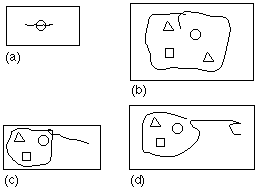
\includegraphics{img/BarfieldF16.png}
\caption{\label{fig:gestes1}Les gestes pour l'édition graphique. (tiré de
(\protect\hyperlink{ref-kurtenbach1991issues}{Kurtenbach and Buxton, 1991}))}
\end{figure}

Pour les artistes, l'entrée gestuelle peut faciliter l'interaction
créative. (\protect\hyperlink{ref-buxton1995chunking}{Buxton, 1995}) a montré un
simple ensemble de gestes pour transcrire la notation musicale. Comme montré
sur la figure \ref{fig:gestes2}, les formes des notes les plus communes (en haut de la
figure) trouvent un équivalent dans l'ensemble des gestes à réaliser (sous
chaque note).

\begin{figure}
\centering
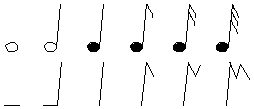
\includegraphics{img/BarfieldF17.png}
\caption{\label{fig:gestes2}Les gestes pour transcrire la notation musicale (tiré de
(\protect\hyperlink{ref-buxton1995chunking}{Buxton, 1995}))}
\end{figure}

\hypertarget{interaction-gestuelle-pure}{%
\subsubsection{Interaction gestuelle pure}\label{interaction-gestuelle-pure}}

Toujours pour (\protect\hyperlink{ref-baudel1995aspects}{Baudel, 1995}), la
reconnaissance de tracés reste limité à reconnaître l'échantillonnage de la
trajectoire d'un point dans le plan (ou l'espace). Le geste effectif réalisé
par l'utilisateur n'est toujours pas pris en compte. Par exemple, la machine
ne distinguera pas si le geste a été effectué de la droite ou de la main
gauche.

Pour accentuer la compréhension du geste par la machine, les dispositifs
de pointage deviennent clairement insuffisants. Il s'agit alors d'utiliser
des gants, ou un système de vision par caméra~; on parlera respectivement de
dispositif intrusif, et non-intrusif~: en effet, dans le cas des gants, on
doit porter un périphérique, tandis qu'avec la caméra, on agit librement.

Une dernière classe d'interaction peut venir s'ajouter. Il s'agit des
systèmes de prise en compte des gestes inconscients. En effet, une partie des
gestes sont de nature inconsciente, et peuvent néanmoins contenir du sens. On
parle alors de dispositifs de suivi du regard, et toujours de vision par
caméra.

\hypertarget{les-puxe9riphuxe9riques-de-sortie-uxe0-retour-haptique}{%
\section{Les périphériques de sortie à retour haptique}\label{les-puxe9riphuxe9riques-de-sortie-uxe0-retour-haptique}}

\hypertarget{historique}{%
\subsection{Historique}\label{historique}}

La télé-robotique est le domaine technologique qui a nécessité la création
de périphériques à retour de force. Le schéma classique est le couple
Maître-esclave . Sheridan (\protect\hyperlink{ref-sheridan1992musings}{Sheridan et al., 1992}) a défini le système
télé-opérateur Maître-esclave comme suit~:

Un télé-opérateur Maître-esclave est constitué de 2
sous-parties~:

\begin{itemize}
\tightlist
\item
  Le dispositif maître, généralement un dispositif
  mécanique plus ou moins anthropomorphique et autorisant de multiples degrés
  de liberté, actionné directement par l'opérateur humain~~;
\item
  Le dispositif esclave, isomorphique au maître, la
  plupart du temps équipé d'une main robotisé ou d'un outil
  spécialisé~.
\end{itemize}

Le retour haptique (uniquement kinesthésique aux débuts~~; on voit
apparaître de plus en plus l'ajout du retour tactile) permet une immersion
beaucoup plus efficace. L'opérateur a de plus en plus l'impression de
manipuler directement l'outil que manipule le périphérique esclave
distant.

Nous pouvons considérer que le premier périphérique à retour de force
vient du monde de la télé-robotique~: en 1952, Groetz et Thompson de l'Argonne
National Laboratory (\protect\hyperlink{ref-goertz1952fundamentals}{Goertz, 1952}) créent
l'Argonne (voir la figure \ref{fig:argonne}), un système
de télémanipulation maître-esclave permettant à un humain de diriger un bras
robotisé dans un milieu hautement dangereux (centrale nucléaire, espace,
fonds sous-marins).

\begin{figure}
\centering
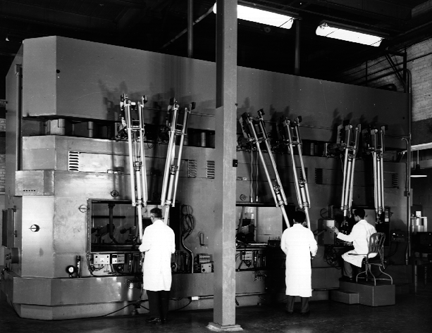
\includegraphics{img/argonne.png}
\caption{\label{fig:argonne}L'argonne}
\end{figure}

Par la suite, d'autres périphériques ont été conçus pour la
télé-robotique, mais il ne s'agit ici que de simuler à distance une
interaction physique qui a lieu dans le monde réel. En 1965,
sous l'impulsion de Ivan Sutherland, Fred Brooks Jr.~et ses collègues de
l'université Chapel Hill de Caroline du Nord, se sont lancés dans le projet
GROPE, visant à atteindre une simulation en temps réel pour la manipulation
tridimensionnelle de molécules virtuelles, en ayant le retour des forces
moléculaires. C'est plus de 20 ans plus tard que Brooks et ses collègues ont
pu atteindre leur but initial (voir figure \ref{fig:MDVI}), grâce à la montée
en puissance des ordinateurs (\protect\hyperlink{ref-brooks1990project}{Brooks Jr et al., 1990}).

\begin{figure}
\centering
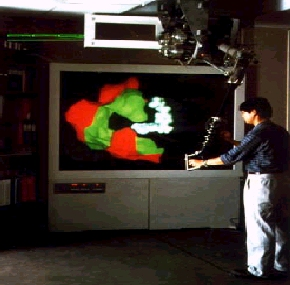
\includegraphics{img/molecular.png}
\caption{\label{fig:MDVI}Molecular Docking Virtual Interface ou MDVI (University of North
Carolina)}
\end{figure}

Enfin, vers la fin des années 70, est apparu le premier prototype de
périphérique effectuant le retour tactile d'une simulation graphique~: le
Sandpaper system développé au MIT (\protect\hyperlink{ref-minsky1995computational}{Minsky, 1995}). Il s'agit d'un
joystick offrant 2 degrés de liberté et rendant à
la fois le retour de force et le retour tactile. Ainsi, il était possible de
faire bouger un curseur au-dessus de divers échantillons de papiers virtuels
et de sentir leurs textures. Cependant, par rapport aux périphériques de
télé-robotique, on note une perte de liberté, puisque l'utilisateur doit
garder une main sur le joystick. En retour, les dispositifs pouvaient
embarquer des outils et mécaniques lourds, puisqu'ils sont posés sur leur
support (en général, le bureau).

\hypertarget{les-puxe9riphuxe9riques-uxe0-retour-haptique}{%
\subsection{Les périphériques à retour haptique}\label{les-puxe9riphuxe9riques-uxe0-retour-haptique}}

Sans prétendre à l'exhaustivité, nous allons présenter quelques
périphériques à retour haptique. Précisons tout d'abord la terminologie
employée (tableau~\protect\hyperlink{cap:Correspondance-terminologique-entre}{2.2}).

\begin{longtable}[]{@{}ll@{}}
\toprule()
Perception & Périphérique \\
\midrule()
\endhead
Kinesthésique & à retour de force / d'effort \\
Tactile & à retour tactile \\
\bottomrule()
\end{longtable}

Table 2.2~: Correspondance
terminologique entre la perception et les périphériques

On peut noter une différence fondamentale entre les deux retours
haptiques~: le retour de force peut s'opposer à un mouvement volontaire de
l'utilisateur,~jusqu'à l'empêcher (s'il est suffisamment fort)~; le
retour tactile ne le peut pas (\href{047-bibliographie.html\#Burdea1992}{Burdea
et~al., 1992}) .

\hypertarget{les-puxe9riphuxe9riques-uxe0-retour-de-force}{%
\subsubsection{Les périphériques à retour de force}\label{les-puxe9riphuxe9riques-uxe0-retour-de-force}}

Nous pouvons distinguer deux grandes familles de périphériques à retour de
force (\protect\hyperlink{ref-casiez2004contribution}{Casiez, 2004}):

\textbf{les~périphériques~à~base~non~fixe}
(\emph{man based}) : ce sont les périphériques
portés par l'utilisateur, de type gant ou exosquelette.

\textbf{les~périphériques~à~base~fixe}
(\emph{ground
based} ou \emph{desk based}) : ils
regroupent les périphériques de type bras, stylos (\emph{probe}), manches
ou souris

Nous allons maintenant voir les principaux dispositifs utilisés dans la
recherche sur l'interaction haptique.

\hypertarget{les-gants}{%
\paragraph{Les gants}\label{les-gants}}

Les gants doivent saisir les mouvements complexes de la main. Ils
autorisent en général un grand nombre de degrés de liberté. En effet chaque
doigt dispose de 4 degrés de liberté, auxquels il faut ajouter les mouvements
de la paume et parfois du poignet. Le retour d'effort permet de ressentir la
rigidité de l'objet mais ne permet pas de ressentir son poids.

Nous pouvons citer le Rutgers Master II qui est basé sur les travaux de
(\protect\hyperlink{ref-burdea1992portable}{Burdea et al., 1992}), et le
CyberGrasp commercialisé par la société Immersion . Ces deux dispositifs se distinguent par
l'emplacement de la structure mécanique. Ainsi, la structure est intérieure à
la paume de la main pour le Rutgers Master II, ce qui empêche l'utilisateur
de fermer totalement la main (figure \ref{fig:rutgers}).

\begin{figure}
\centering
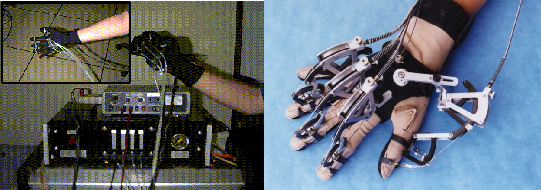
\includegraphics{img/rutgers.png}
\caption{\label{fig:rutgers}Les gants Rutgers Master II et CyberGrasp}
\end{figure}

\hypertarget{les-bras-mauxeetres}{%
\paragraph{Les bras maîtres}\label{les-bras-mauxeetres}}

Les bras maîtres sont principalement utilisés dans les applications de
télé-opérations. Sur la figure \ref{fig:dextros}
apparaît le Dextrous Arm Master créé par SARCOS, l'une des entreprises
pionnières dans le domaine. Ces systèmes, placés soit sur une table ou sur le
sol, sont capables de fournir des forces puissantes à l'utilisateur. Ils sont
également utilisés dans les applications de réalité virtuelle.

\begin{figure}
\centering
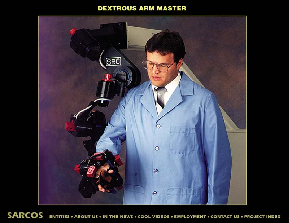
\includegraphics{img/dextroslarge.png}
\caption{\label{fig:dextros}Le SARCOS Dextrous Arm Master}
\end{figure}

\hypertarget{les-stylos-uxe0-retour-de-force}{%
\paragraph{Les stylos à retour de force}\label{les-stylos-uxe0-retour-de-force}}

Ce sont des périphériques proposant au minimum trois degrés de liberté en
entrée (le déplacement du stylet dans l'espace), mais le plus souvent six~; et
3 degrés de liberté en sortie (c'est à dire sur le retour de force), et
parfois six. La figure \ref{fig:degres} illustre
les différentes possibilités en terme de degrés de liberté.

\begin{figure}
\centering
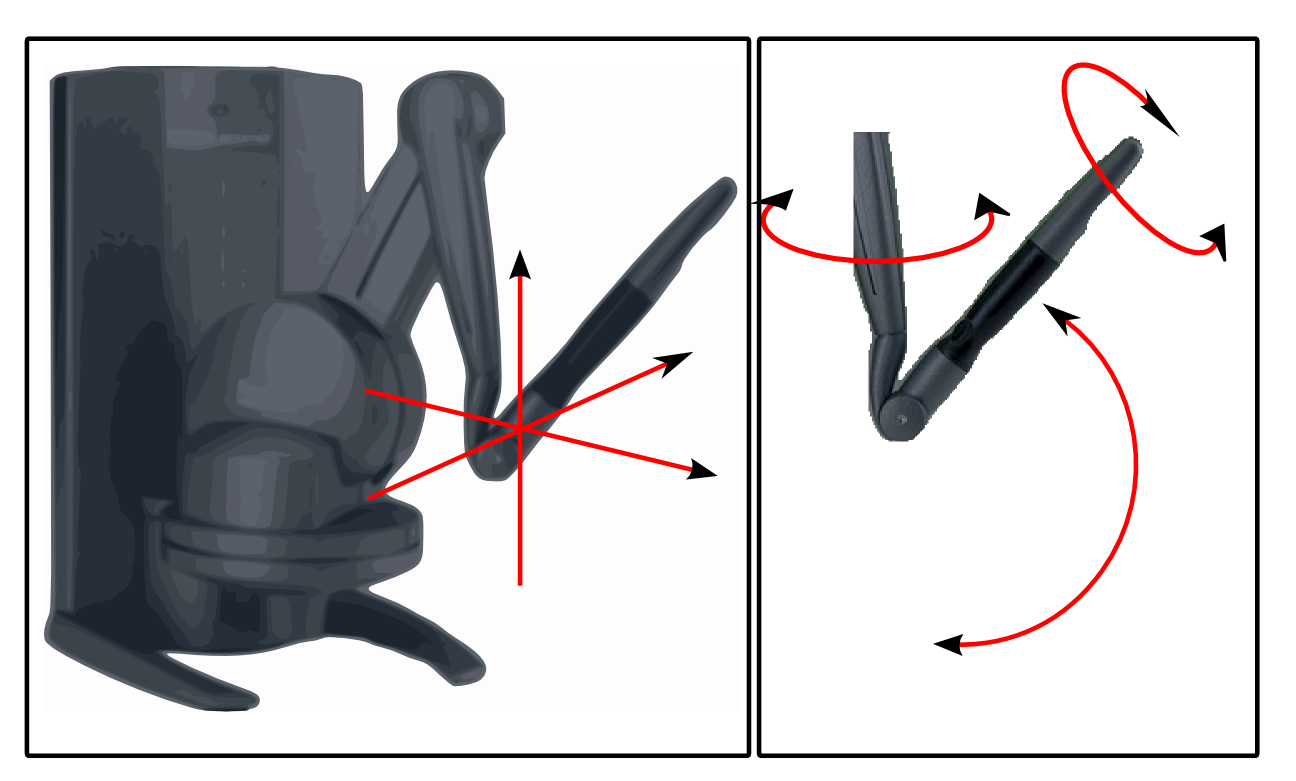
\includegraphics{img/DoF.png}
\caption{\label{fig:degres}Les degrés de liberté sur un bras à retour de force}
\end{figure}

Le périphérique le plus utilisé dans les laboratoires est le PHANTOM
(figure \ref{fig:PHANTOM}), créé et commercialisé par
Sensable Inc.

\begin{figure}
\centering
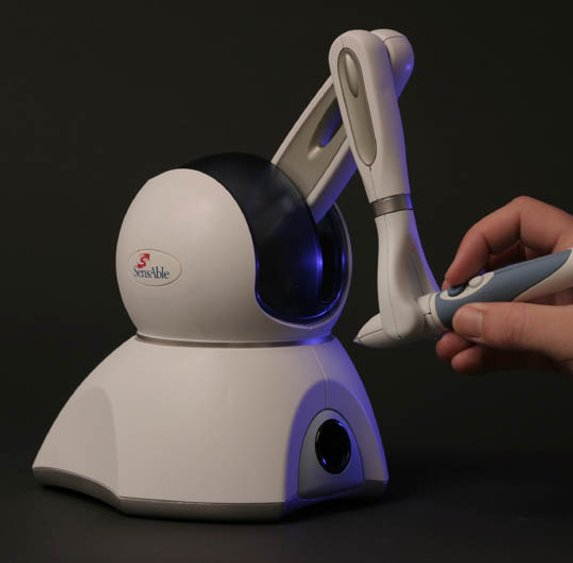
\includegraphics{img/phantom-omni.png}
\caption{\label{fig:PHANTOM}le PHANTOM, dans sa version omni.}
\end{figure}

Son maniement s'effectue grâce un stylet situé à l'extrémité du
périphérique ou en insérant le bout de son doigt dans un dé. Il est alors
possible, grâce à une excellente résolution spatiale de ressentir les
sensations que l'on aurait à toucher un mur lisse, un coin pointu, une sphère
caoutchouteuse ou encore une surface texturée.

Nous pouvons citer le Virtuose 3D, le Delta Haptic et le Freedom 6S
(figures \ref{fig:virtuose}, \ref{fig:deltahaptique} et
\ref{fig:freedom6s}), également utilisés dans les laboratoires.

\begin{figure}
\centering
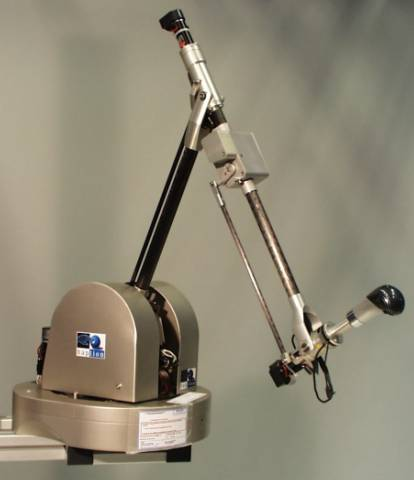
\includegraphics{img/virtuose.jpg}
\caption{\label{fig:virtuose}Le Virtuose 3D}
\end{figure}

\begin{figure}
\centering
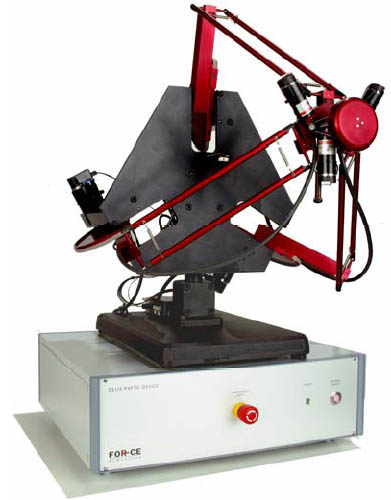
\includegraphics{img/delta_6dof.jpg}
\caption{\label{fig:deltahaptique}le Delta Haptic}
\end{figure}

\begin{figure}
\centering
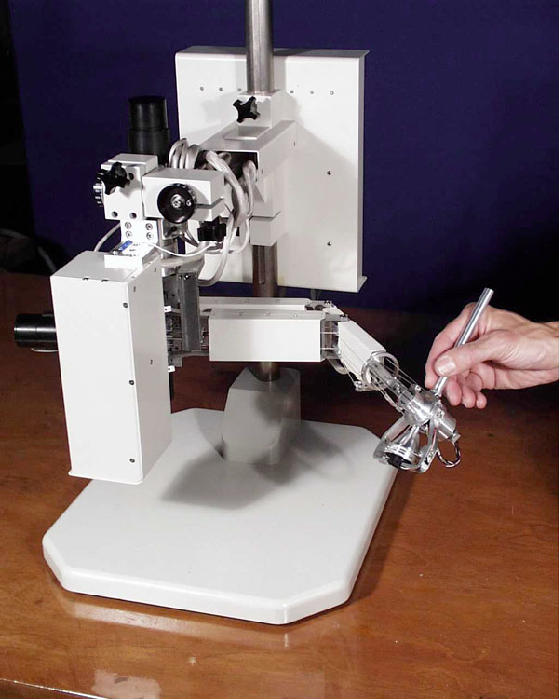
\includegraphics{img/freedom6s.png}
\caption{\label{fig:freedom6s}le Freedom 6S}
\end{figure}

Précisons que les périphériques de type PHANTOM sont à la 3D ce que la
souris à la 2D~: des \textbf{périphériques de pointage} : seul un point est
déplacé dans l'espace.

\hypertarget{les-souris-uxe0-retour-de-force}{%
\paragraph{Les souris à retour de force}\label{les-souris-uxe0-retour-de-force}}

Les souris à retour de force sont des dispositifs à deux degrés de
liberté. Nous pouvons citer la Wingman Force Feedback Mouse
(figure \ref{fig:wingman}), conçue par Immersion, et
commercialisée par Logitech.

\begin{figure}
\centering
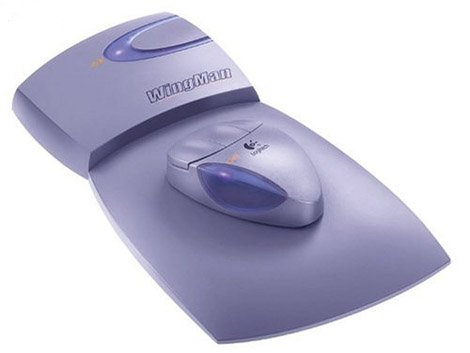
\includegraphics{img/wingFFM.jpg}
\caption{\label{fig:wingman}Wingman Force Feedback Mouse}
\end{figure}

La souris proprement dite est solidaire de son socle. De fait, la surface
de travail de cette souris est très réduite~: 1,9 cm par 2,5 cm. Enfin,
la souris peut générer des forces pouvant atteindre 1N.

La souris Wingman force Feedback a originalement été conçue pour les jeux
vidéos, mais ses possibilités et son faible coût l'ont rendue populaire dans
les recherches sur l'accessibilité auprès des personnes non-voyantes
(\protect\hyperlink{ref-yu2001haptic}{Yu et al., 2001}) (\protect\hyperlink{ref-gardner2001smart}{Gardner and Bulatov, 2001}) (\protect\hyperlink{ref-tornil2004use}{Tornil and Baptiste-Jessel, 2004})).

\hypertarget{les-puxe9riphuxe9riques-uxe0-retour-tactile}{%
\subsubsection{Les périphériques à retour tactile}\label{les-puxe9riphuxe9riques-uxe0-retour-tactile}}

Les dispositifs tactiles sont bien entendu basés sur \href{007-le-systeme-haptique-cote-perception-la-somesthesie.html\#toc3}{les perceptions
tactiles}.
Nous pouvons par exemple rappeler, que la perception
tactile est le fait de trois classes de récepteurs~: les thermorécepteurs,
les nocirécepteurs et les mécanorécepteurs. Du côté de la machine, ce sont
surtout des dispositifs répondant aux mécanorécepteurs, et donc à nos
capacités de discrimination tactile, qui ont été conçus. On peut pourtant
citer les travaux du Dr Suichi Ino, de l'université d'Hokkaido, qui cherche à
créer un système de rendu de la température. Le Temperature Display, par
exemple autorise un intervalle de température allant de 10°C à 60°C à une
précision de 0.1°C pour un dispositif ne pesant que 30 grammes.

Pour le reste, donc, les dispositifs sont surtout axés sur la
discrimination tactile. Et la principale approche pour rendre un élément
tactile est celle visible sur la figure \ref{fig:afficheur}.On peut y voir
une cellule d'affichage tactile. Cette cellule est composée de petits picots
capables de monter ou descendre sur leur axe. Il ainsi possible de dessiner
des petits motifs en relief.

\begin{figure}
\centering
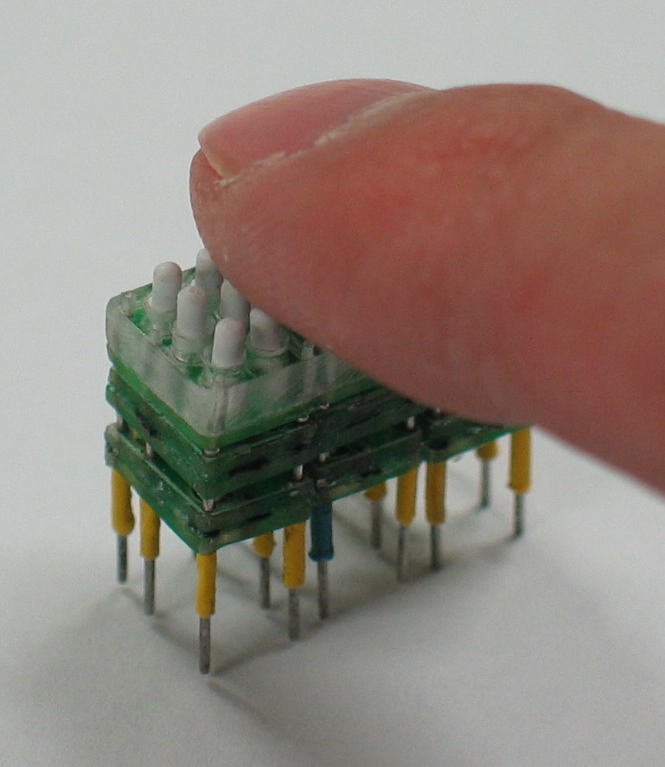
\includegraphics{img/braille_cell3.jpg}
\caption{\label{fig:afficheur}Une cellule d'afficheur tactile}
\end{figure}

Les afficheurs brailles (figure \ref{fig:plagebraille}) utilisent
ces cellules. Comme un caractère
braille est composé de 8 points (pour le braille informatique), une cellule
est composée de 8 picots. Il s'agit ensuite d'accoler un certain nombre de
cellules (selon les modèles, de 20 à plus de 80 cellules) pour afficher
plusieurs caractères brailles, et donc, un mot, une phrase.

\begin{figure}
\centering
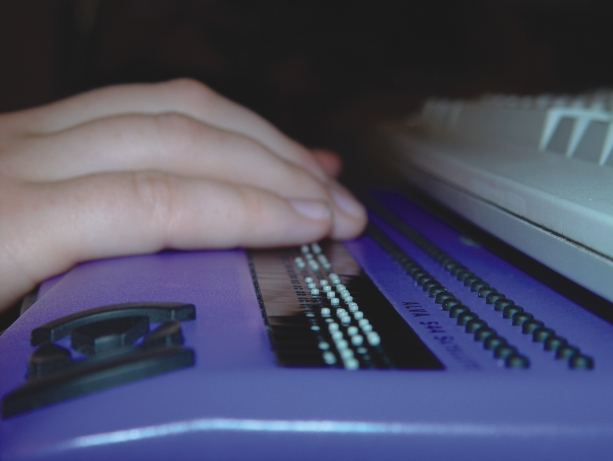
\includegraphics{img/braille-1.jpg}
\caption{\label{fig:plagebraille}Une plage braille}
\end{figure}

Toujours dans la même approche, les sociétés ABTIM \footnote{\url{http://www.abtim.com}} et
KGS \footnote{\url{http://www.kgs-america.com/dvs.htm}} ont équipé de cellules des surfaces
plus grande. Il ont ainsi réalisé des systèmes capables de reproduire des
dessins en relief (figure \ref{fig:tactiledisplay}).

\begin{figure}
\centering
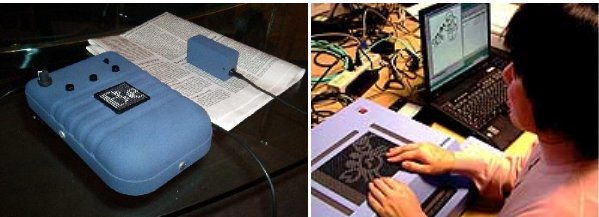
\includegraphics{img/tactileDisplay.jpg}
\caption{\label{fig:tactiledisplay}(gauche) : l'ADVANCED DISPLAYS for the BLIND de ABTIM~;
(droite) : le DotView de KGS}
\end{figure}

Pour terminer cette partie, nous pouvons évoquer une autre classe de
périphériques, qui exploite les capacités tactiles en sortie (de l'ordinateur
vers l'humain), et les capacités kinesthésiques en entrée (de l'humain vers
la machine). Il s'agit souvent d'adapter une cellule braille sur un
dispositif de pointage (\href{047-bibliographie.html\#Lecolinet2005}{Lecolinet et
Mouret, 2005}). D'autres exemples sont visibles sur la
figure \ref{fig:couplage}.

\begin{figure}
\centering
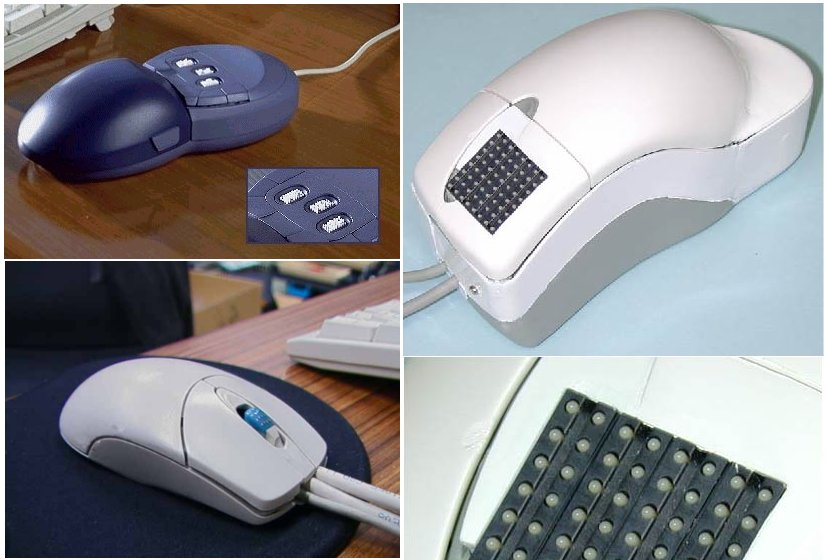
\includegraphics{img/sourisTactile.jpg}
\caption{\label{fig:couplage}Le couplage des dispositifs de pointage avec le mode
tactile}
\end{figure}

\hypertarget{les-applications-du-retour-haptique}{%
\section{Les applications du retour haptique}\label{les-applications-du-retour-haptique}}

\hypertarget{perception}{%
\subsection{La perception via une interface haptique}\label{perception}}

D'un point de vue général, il s'avère que les dispositifs actuels
limiteront les procédures d'exploration haptique. L'utilisateur est en effet
obligé d'adopter des stratégies afin d'extraire les propriétés des objets. Et
ceci est particulièrement notable sur les dispositifs nécessitant la
manipulation d'un activateur comme le manche du joystick ou le stylet du
PHANTOM (\protect\hyperlink{ref-jansson1999phantom}{Jansson and Billberger, 1999}). De plus, la technologie même est un facteur
limitant~: (\protect\hyperlink{ref-wall2004investigation}{Wall, 2004}) a ainsi montré que les moteurs du
PHANTOM étaient inadéquats pour générer des textures très fines nécessitant
des hautes fréquences.

En se référant aux \protect\hyperlink{conjuguent}{procédures d'exploration haptique} proposées
par (\protect\hyperlink{ref-lederman1987haptic}{Lederman et al., 1987}), (\protect\hyperlink{ref-wall2004investigation}{Wall, 2004}) a dressé le
tableau \ref{tab:possibilite}, qui montre les possibilités et les
impossibilités, lorsque l'on manipule un dispositif de pointage. Finalement,
(\protect\hyperlink{ref-lederman2004haptic}{Lederman and Klatzky, 2004}) ont également montré que la rigidité du stylet limitait
également la perception (par rapport à un stylet flexible).

\begin{longtable}[]{@{}
  >{\raggedright\arraybackslash}p{(\columnwidth - 2\tabcolsep) * \real{0.3367}}
  >{\raggedright\arraybackslash}p{(\columnwidth - 2\tabcolsep) * \real{0.6633}}@{}}
\caption{\label{tab:possibilite} Les possibilités des mouvements d'exploration avec un
périphérique de pointage}\tabularnewline
\toprule()
\endhead
\textbf{Mouvements d'exploration} & \textbf{Possibilité avec un dispositif de pointage} \\
Le mouvement latéral (textures) & Possible, bien que les caractéristiques des textures varient \\
& temporellement (vibration) et non pas spatialement \\
La pression & Possible \\
Le contact statique & Possible, bien qu'il n'y ait pas de retour de température, \\
& ou de forces distribuées pour générer des étirements \\
Le maintient & Possible en attachant l'objet simulé à la place de l'activateur \\
L'enveloppement & Non possible en l'absence de plusieurs points de contact \\
Le suivi de contours & Possible, mais très difficile du fait d'une zone de contact \\
& réduite à un point \\
\bottomrule()
\end{longtable}

Pour l'anecdote, (\protect\hyperlink{ref-jansson2000haptic}{Jansson, 2000}) a
suggéré qu' obtenir une information par l'intermédiaire d'un affichage
haptique tel que le PHANTOM, était semblable à obtenir de l'information d'un
écran d'ordinateur en déplaçant sur celui-ci une feuille de papier percée
d'un simple petit trou .

Concernant la mémorisation, \href{047-bibliographie.html\#Jansson1999}{(Jansson et
K., 1999)} ont montré qu'une phase, même très courte, d'initiation à
l'utilisation d'un dispositif comme le PHANTOM, permettait une nette
amélioration des performances.

Comme nous allons maintenant le voir, les applications utilisant de tels
dispositifs, malgré leurs défauts, se multiplient dans de nombreux
domaines.

\hypertarget{lintuxe9gration-du-mode-haptique-dans-linteraction-avec-la-machine}{%
\subsection{L'intégration du mode haptique dans l'interaction avec la machine}\label{lintuxe9gration-du-mode-haptique-dans-linteraction-avec-la-machine}}

Le système haptique humain a un rôle important à jouer dans l'interaction
homme-machine. \textbf{A l'inverse des systèmes visuels et auditifs, le sens
haptique est capable à la fois de percevoir et d'agir sur l'environnement}
et est une partie importante de la plupart des activités humaines. La
figure \ref{fig:interactionhaptique} illustre la double boucle d'interaction
liée au système haptique~: l'homme et la machine agissent et perçoivent sur
le mode haptique, en même temps. Les schémas de fonctionnement pour l'homme
et pour la machine sont très similaires~: il y a dans les deux cas une boucle
action-réaction entre le monde extérieur, et le système de décision ~; c'est
à l'intersection des deux boucles que se situe l'interaction.

\begin{figure}
\centering
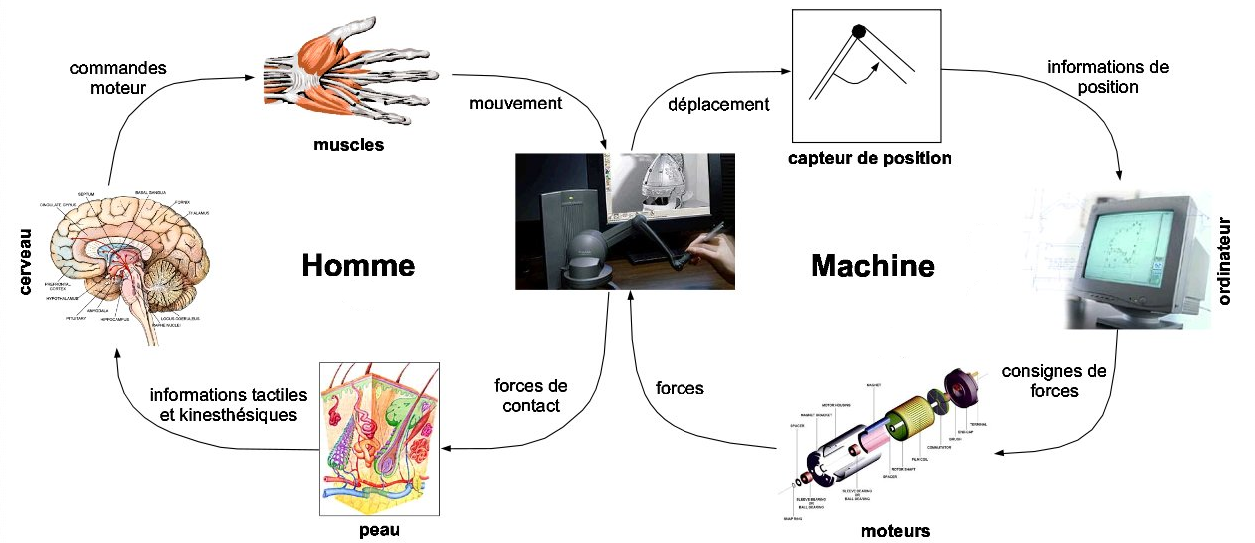
\includegraphics{img/retourhaptic.png}
\caption{\label{fig:interactionhaptique}Interaction haptique entre l'homme et la machine
(tiré de (\protect\hyperlink{ref-casiez2004contribution}{Casiez, 2004}))}
\end{figure}

Dans cette partie, nous allons passer en revue quelques applications
concrètes basées sur le mode haptique. On pourra revenir à
\protect\hyperlink{historique}{cette page} pour un historique sur les débuts du retour de
force. On rappelle qu'initialement, c'est en télé-robotique que les
dispositifs à retour de force sont apparus.

\hypertarget{le-retour-haptique-comme-technique-dinteraction}{%
\subsubsection{Le retour haptique comme technique d'interaction}\label{le-retour-haptique-comme-technique-dinteraction}}

(\protect\hyperlink{ref-miller1999design}{Miller and Zeleznik, 1999}) ont identifié 4 utilisations possibles du retour haptique~:

\begin{enumerate}
\def\labelenumi{\arabic{enumi}.}
\tightlist
\item
  \emph{Anticipation} (Anticipation): force
  résistante annonçant l'imminence d'un événement.
\item
  \emph{Indication} (Suivi) : force donnant
  l'indication qu'une action est en cours.
\item
  \emph{Follow-through} (Accomplissement): force
  donnant l'indication à l'utilisateur qu'un événement s'est produit.
\item
  \emph{Guidance} (Guidage): guidage/contrainte du
  geste de l'utilisateur.
\end{enumerate}

\hypertarget{le-retour-haptique-aspect-logiciel}{%
\subsubsection{Le retour haptique~: aspect logiciel}\label{le-retour-haptique-aspect-logiciel}}

Afin de manipuler les dispositifs, les fabriquants ont mis à la
disposition des programmeurs, des bibliothèques de programmation
spécialisées.

Immersion Corporation™, le fabriquant de la souris Wingman Force Feedback
Mouse™, propose ainsi l'Immersion Touchsense SDK. Cette bibliothèque permet
de piloter tout un ensemble de périphériques~(souris, joysticks, volants
et manettes de jeux) chez de nombreux constructeurs (Microsoft™, Logitech™,
Genius™, ThrustMaster™, Saitek™, Gravis™). De plus, une des particularités de
ce SDK (\emph{Software Developpment Kit}) est qu'il dispose d'un plugin
pour les navigateurs Web. Ainsi, il est possible d'augmenter une page Web,
avec des retours de force. Les navigateurs supportés sont Microsoft™Internet
Explorer et Netscape™. Une version pour les navigateurs basés sur le moteur
Gecko (Mozilla™, Firefox) existe, mais est encore en phase de
développement.

Sensable™, le concepteur des PHANTOMs, propose plusieurs bibliothèques de
programmation~: Le Ghost SDK, et les HDAPI et HLAPI. Le Ghost SDK est basé
sur un moteur de rendu du toucher, à partir d'une scène 3D. Par exemple, il
dispose d'un lecteur de fichiers VRML (Virtual Reality Markup Language~:
langage de description de scènes 3D), et l'on peut très rapidement toucher
les objets de la scène, avec un PHANTOM. Cependant, il peut être intéressant
de se passer d'une base tridimensionnelle pour générer des effets. Ainsi,
Sensable™a proposé les bibliothèques HDAPI et HLAPI (pour \emph{Haptic Device
API} et \emph{Haptic Library API}). La bibliothèque HDAPI permet un
contrôle direct des paramètres de fonctionnement du périphérique~: les
positions, orientations et vitesses des différents éléments du dispositif,
l'accès aux systèmes de coordonnées internes des moteurs, les températures
des moteurs\ldots{} Comparé au Ghost SDK, le HDAPI autorise beaucoup plus de
liberté et de précision lors de la création des effets. Il peut cependant
s'avérer fastidieux de créer des effets à partir d'autant de paramètres.
C'est pour cette raison que Sensable™a conçu le HLAPI. Il s'agit d'un
bibliothèque intermédiaire entre les deux autres. À l'instar du GHOST SDK, on
part d'une scène 3D, mais cette fois, la scène est décrite en OpenGL. Ceci
permet un contrôle encore très précis.

Nous pouvons également citer le H3D API de SenseGraphics \footnote{\url{http://www.sensegraphics.se}}.
C'est une bibliothèque de programmation haptique open-source (licence GPL
dans un cadre de recherche), basée sur le format de fichier X3D (il s'agit du
format de description de formes 3D, basé sur XML~; c'est le successeur du
VRML). Pour le moment, cette bibliothèque ne supporte que les PHANTOMs.

\hypertarget{le-retour-haptique-uxe0-quoi-cela-ressemble}{%
\subsubsection{Le retour haptique~: à quoi cela ressemble ?}\label{le-retour-haptique-uxe0-quoi-cela-ressemble}}

Jusqu'ici, nous avons discuté de périphériques à retour de force, mais
nous n'avons pas dit en quoi consistait le retour de force. La partie
précédente a présenté quelques bibliothèques de programmation qui permettent
de concevoir des effets de retour de force, effets dont nous allons
maintenant présenter les grandes familles (en notant bien, que les
bibliothèques de programmation permettent de combiner ces différents
effets).

\textbf{Le~contact~ponctuel~:}
il s'agit de l'effet le plus classique, mais
aussi le plus étudié. L'idée est de générer une force dans un dispositif à
retour de force, pendant qu'on le manipule, de manière à simuler le contact
avec un objet du monde virtuel, comme s'il existait. Par exemple, avec un
périphérique type PHANTOM, imaginons que la manipulation du stylet amène le
curseur au contact d'une forme virtuelle ~; à cet instant, les moteurs du
PHANTOM se durcissent afin de limiter les mouvements de l'utilisateur selon
certaines directions. On aura alors l'illusion de rentrer en contact avec
un objet physique.

\textbf{Le~cloisonnement~:}
Il s'agit de définir une zone (souvent
rectangulaire ou elliptique), qui aura une frontière entièrement
paramétrable. Cet effet possède alors une notion d'intérieur et
d'extérieur. On peut par exemple donner la possibilité ou non, au pointeur
de rentrer ou de sortir de la zone. Il peut s'agir également de définir une
zone d'attraction, qui attirera le curseur en son centre lorsqu'il passe à
une certaine distance.

\textbf{Les~effets~dynamiques~:}
Ce sont des effets dont les paramètres évoluent
dynamiquement selon les propriétés du geste de l'utilisateur. Par exemple,
une certaine friction peut être simulée, en fonction de la vitesse
instantanée, ou du rayon de courbure. Autre exemple, le périphérique peut
empêcher l'utilisateur des changements de direction trop brusques~: on
simule ainsi l'inertie du déplacement d'un objet lourd.

\textbf{Les~effets~de~texture~:}
Ces effets permettent de simuler des textures.
Celles-ci peuvent être synthétisées grâce à un certain nombre de paramètres
(fréquence, amplitude, directions\ldots), ou bien simulée depuis une image
réelle de façon similaire à ce que réalise une bump-map en image de
synthèse, c'est à dire une image ou l'intensité d'une nuance (du noir au
blanc par exemple) code l'altitude ou la profondeur.

\hypertarget{quelques-applications-du-retour-haptique}{%
\subsection{Quelques applications du retour haptique}\label{quelques-applications-du-retour-haptique}}

\hypertarget{la-muxe9decine-et-la-ruxe9uxe9ducation}{%
\subsubsection{La médecine et la rééducation}\label{la-muxe9decine-et-la-ruxe9uxe9ducation}}

Depuis le début des années 90, la médecine est devenue un champ
d'application du retour haptique. Plusieurs pratiques peuvent nécessiter
l'utilisation de dispositifs à retour de force.

\textbf{La~palpation~des~tissus~:}
Elle correspond à la première étape d'une
consultation~: le diagnostic. Et la forme la plus traditionnelle de
diagnostic est la palpation des organes et des tissus du patient. En 1994,
(\protect\hyperlink{ref-langrana1994dynamic}{Langrana et al., 1994}) ont pour
la première fois utilisé un périphérique à retour haptique, \href{016-les-peripheriques-de-sortie-a-retour-haptique.html\#sub:Les-gants}{le Rutger
Master}, pour palper un genou virtuel. Depuis, les
outils ont évolués, et les applications de télé-diagnostic se
généralisent.

\textbf{La~télé-chirurgie~:}
La télé-chirurgie est un des grands axes de la
recherche sur les périphériques haptiques. Le praticien peut ainsi
intervenir au cours d'une opération alors qu'il ne se trouve pas sur
place.

\textbf{La~rééducation~:}
Cette approche de l'utilisation des dispositifs
à retour de force est très intéressante. En général, les dispositifs de
rééducation utilisent des périphériques sortis de leurs contextes habituels
d'utilisation. \href{047-bibliographie.html\#Reinkensmeyer2000}{(Reinkensmeyer
et~al., 2000)} ont par exemple utilisé un joystick à retour de
force tel qu'on peut en trouver dans le commerce, pour rééduquer l'acuité
motrice d'un patient ayant subit un accident cérébral.

\hypertarget{la-moduxe9lisation-dobjets-virtuels}{%
\subsubsection{La modélisation d'objets virtuels}\label{la-moduxe9lisation-dobjets-virtuels}}

Un logiciel de modélisation tridimensionnelle nommé
FreeForm \footnote{\url{http://www.sensable.com/products/3ddesign/concept/index.asp}}, a été
présenté par Sensable Technologies Inc.~Ce système se base sur une métaphore du
sculpteur~: l'utilisateur se sert du PHANTOM pour sculpter une pierre
virtuelle présentée à l'écran, et rendue par un retour de force.

De manière similaire, InTouch (\protect\hyperlink{ref-gregory2000intouch}{Gregory et al., 2000}) est un logiciel de
modélisation 3D. Il permet également le dessin sur un volume
(figure \ref{fig:intouch}).

\begin{figure}
\centering
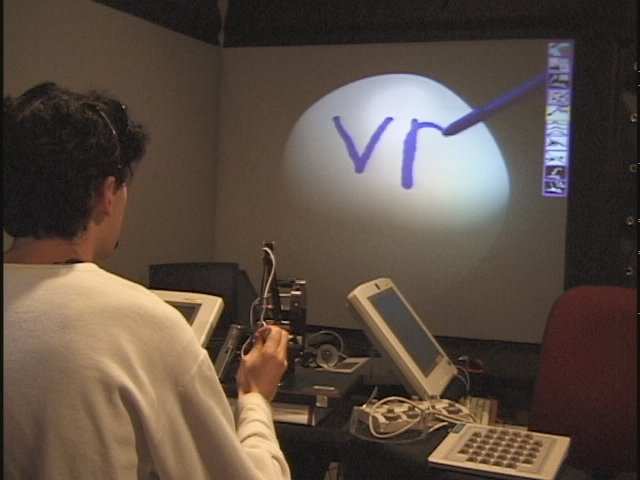
\includegraphics{img/systemSetup.jpg}
\caption{\label{fig:intouch}Le logiciel inTouch}
\end{figure}

\hypertarget{le-travail-collaboratif}{%
\subsubsection{Le travail collaboratif}\label{le-travail-collaboratif}}

L'utilisation du mode haptique dans une collaboration en environnement
virtuel, peut permettre une amélioration, notamment de la conscience que l'on
doit avoir de travailler avec quelqu'un (\protect\hyperlink{ref-basdogan2000experimental}{Basdogan et al., 2000}).

(\protect\hyperlink{ref-sallnas2003collaboration}{Sallnäs and Zhai, 2003}) ont montré
également une diminution du taux d'erreur lors d'une tâche de pointage
collaboratif lorsqu'un retour haptique était rendu (pour des temps identiques
avec ou sans retour haptique).

On peut noter qu'il s'agit d'une classe d'application qui nécessite des
recherches pluridisciplinaires~: rendus haptiques, bien sûr, mais aussi
réseaux et traitement du signal. Par exemple, lorsque la collaboration se
fait via un réseau, il faut anticiper, afin d'atténuer le délai temporel
qu'il peut y avoir entre les deux machines. (\protect\hyperlink{ref-belghit2003amelioration}{Belghit, 2003}) a ainsi utilisé une forme
modifiée du LPC (Linear Prediction Coding) pour améliorer l'ergonomie du
télégeste.

\hypertarget{lentrauxeenement}{%
\subsubsection{L'entraînement}\label{lentrauxeenement}}

Un des intérêts du retour haptique est qu'il peut simuler l'utilisation
d'outils du monde réel. C'est donc tout naturellement que des simulateurs, ou
des plate-formes d'entraînement, ont pu être conçues.

(\protect\hyperlink{ref-williams2004implementation}{Williams et al., 2004}) ont par
exemple mis au point un système d'entraînement au diagnostic du mal de dos.
Leurs recherches les ont amené à créer un moyen de playback haptique. Le
playback haptique consiste à enregistrer les mouvements réalisés par une
personnes, puis de les refaire exécuter par le dispositif haptique (dans ce
cas, il s'agit du PHANTOM). De cette manière, les étudiants pouvaient suivre
les mouvements d'un expert, avant de réaliser leur propre exercice. On peut
quasiment parler de retour de geste, de la part de la machine.

Le centre lavalois de ressources
technologiques \footnote{CLARTE~: \url{http://www.clarte.asso.fr/}} a proposé le système VTT
(\emph{Virtual Technical Trainer}) qui est un simulateur de machine outils.
Ce simulateur a comme raison d'être l'actuelle utilisation quasi systématique
de machines à commandes numériques. Or ces dernières ont pour particularité
d'introduire une distance à la matière telle que l'apprenant perd toute
notion des contraintes mécaniques dans les tâches réalisées par les machines
d'usinage.

\hypertarget{le-domaine-artistique}{%
\subsubsection{Le domaine artistique}\label{le-domaine-artistique}}

Le retour de force a souvent été utilisé dans les domaines artistiques.
Comme dans la partie précédente, cela peut consister en la simulation d'un
instrument réel, comme pour le projet dAb (figure \ref{fig:dab})~:
le dispositif utilisé est un PHANTOM, et il s'agit d'imiter les sensations
que l'on a lors du maniement de pinceaux.

Dans une approche très différente, le projet PHASE (Plate-forme Haptique
d'Application Sonore pour l'Eveil Musical (figure \ref{fig:phase})
propose un moyen de création complètement nouveau. Le retour haptique est
utilisé pour faire sentir les éléments d'un monde virtuel que l'on rencontre
pendant l'exploration de celui-ci.

\begin{figure}
\centering
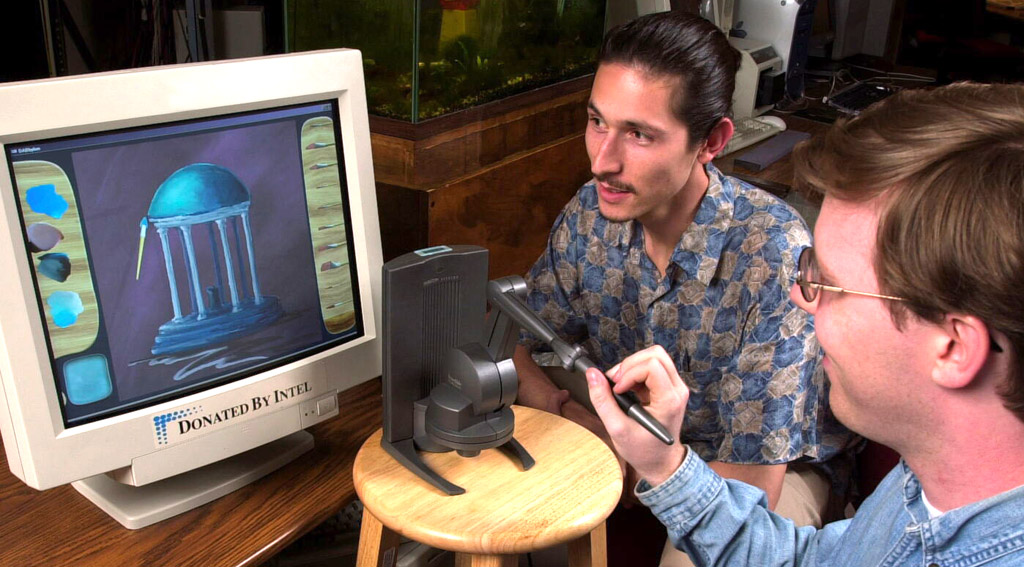
\includegraphics{img/dab_system_scheib_baxter-cropped.jpg}
\caption{\label{fig:dab}Le système dAb
(\protect\hyperlink{ref-bill2001interactive}{Bill et al., 2001})}
\end{figure}

\begin{figure}
\centering
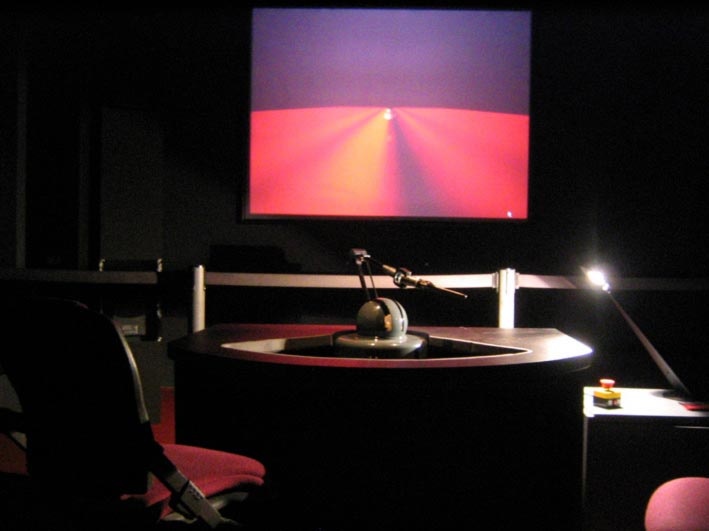
\includegraphics{img/InstalPhaseCGP.jpg}
\caption{\label{fig:phase}La Plate-forme PHASE (\protect\hyperlink{ref-rodet2005phase}{Rodet et al., 2005})}
\end{figure}

\hypertarget{conclusion-1}{%
\section{Conclusion}\label{conclusion-1}}

Dans ce chapitre, nous avons parcouru quelques aspects de l'interaction
homme-machine, en orientant notre discours vers le potentiel, les
utilisations et les défauts, des interactions basées sur le mode haptique.
Une dernière utilisation reste cependant à détailler~: il s'agit de l'aide
aux personnes non-voyantes, mais tout ceci sera étudié et défini dans le
chapitre~\href{025-chapitre-4-vers-l-accessibilite.html}{4}.

Pour le moment, nous avons vu que le retour haptique était une possibilité
d'amélioration de l'immersion dans un monde virtuel, un outil d'entraînement,
ou encore un nouveau moyen d'expression artistique.

Nous allons maintenant nous rappeler qu'à l'origine, le retour de force a
été utilisé dans le but d'améliorer les performances motrices humaines dans
les environnements virtuels et télé-robotiques (\protect\hyperlink{ref-rosenberg1993virtual}{Rosenberg, 1993})
(\protect\hyperlink{ref-sheridan1992musings}{Sheridan et al., 1992}). Aussi, nous allons étudier cet
aspect sur un simple bureau virtuel, dans un schéma d'interaction WIMP, où
l'action gestuelle principale, est le geste de pointage. En effet, sur les
systèmes informatiques courant (Windows, Mac OS, Linux), la l'interaction est
basée sur les mouvements de la souris et les cibles à cliquer (boutons,
menus, fenêtres). Aussi, un des axes de recherches phare dans le domaine de
l'IHM, consiste à essayer d'améliorer les gestes de pointages, c'est à dire,
réduire le temps d'acquisition d'une cible à l'aide d'un dispositif de
pointage.

\hypertarget{performances-du-retour-de-force-sur-le-pointage}{%
\chapter{Performances du retour de force sur le pointage}\label{performances-du-retour-de-force-sur-le-pointage}}

\hypertarget{introduction-amuxe9liorer-la-vitesse-de-pointage}{%
\section{Introduction~: améliorer la vitesse de pointage}\label{introduction-amuxe9liorer-la-vitesse-de-pointage}}

Du fait des interfaces WIMP (\emph{Windows, Icons, Menu, Pointing
Devices)}, une grande partie de l'interaction avec les ordinateurs est
actuellement effectuée à l'aide de la souris. La tâche typique est~:

\begin{enumerate}
\def\labelenumi{\arabic{enumi}.}
\tightlist
\item
  repérage de la cible
\item
  déplacement de la souris au dessus de la cible
\item
  clic sur la cible
\end{enumerate}

La cible pouvant être une icône, un élément d'un menu, une partie d'une
fenêtre. Les moyens quantitatifs avec lesquels nous pouvons évaluer les performances
motrices humaines lors d'une tâche d'acquisition de cible sont basés sur les
recherches de Fitts (voir \ref{fitts}).

Pour rappel, la loi de Fitts énonce que le temps du mouvement \(T\) requis
pour sélectionner une cible de taille \(W\) situé à une distance \(A\) est~:
(\protect\hyperlink{ref-fitts1954information}{Fitts, 1954})

\[ MT=a+b\log_{2}(A/W+1)\]

Le problème de l'amélioration du temps de pointage est un domaine de
recherche actuellement très actif. On pourra se rapporter à
(\protect\hyperlink{ref-balakrishnan2004beating}{Balakrishnan, 2004}) pour une étude exhaustive des moyens employés pour
diminuer ce temps. En considérant l'équation (\eqref{eq:mackenzieID}), réduire
\(MT\) peut s'obtenir en diminuant la distance \(A\), en augmentant la taille \(W\),
ou adaptant les deux en même temps.

Par exemple, pour diminuer la distance \(A\), on peut utiliser des menus
circulaire (\emph{pie menus}). (\protect\hyperlink{ref-callahan1988empirical}{Callahan et al., 1988}) ont comparé ces
menus aux traditionnels menus linéaires que l'on retrouve dans tous nos
systèmes d'exploitation, et a observé une amélioration des temps de pointage
de 15 à 20\%. (\protect\hyperlink{ref-baudisch2003drag}{Baudisch et al., 2003}) ont, quant à eux, proposé de diminuer
temporairement cette distance, en étirant les icônes cibles vers le curseur
de la souris (figure \ref{fig:diminution}).

\begin{figure}
\centering
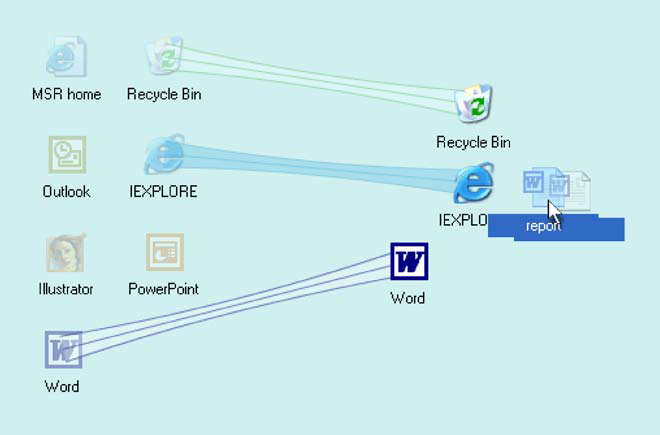
\includegraphics{img/toto-002.png}
\caption{\label{fig:diminution}Diminution de la distance entre l'icône et ses
cibles}
\end{figure}

Pour augmenter la taille de la cible \(W\), il y a
eu plusieurs façons de faire~: (\protect\hyperlink{ref-worden1997making}{Worden et al., 1997}) ont proposé l'utilisation
d'un curseur-région (figure \ref{fig:areacursor}), à l'inverse
d'un curseur-point tel que nous utilisons en manipulant notre souris. Il y a
aussi la possibilité de dilater la cible à l'approche du curseur
(\protect\hyperlink{ref-mcguffin2002acquisition}{McGuffin and Balakrishnan, 2002}), à l'instar de ce qui se passe sur la barre
d'application (le Dock) du système MacOSX d'Apple.

\begin{figure}
\centering
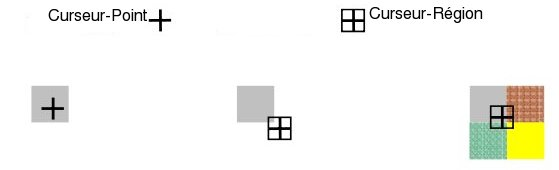
\includegraphics{img/areaCursor.jpg}
\caption{\label{fig:areacursor}Les curseurs-régions de (\protect\hyperlink{ref-worden1997making}{Worden et al., 1997}) ; à gauche~:
la sélection avec un curseur-point a lieu lorsque l'intersection des
deux segments est sur la cible ; au milieu~: la sélection avec un
curseur-région a lieu dès qu'une partie du curseur intersecte la
cible ; à droite~: lorsque plusieurs cibles se trouvent sous le
curseur-région, c'est le comportement d'un curseur-point qui est
utilisé}
\end{figure}

Enfin, (\protect\hyperlink{ref-blanch2004semantic}{Blanch et al., 2004}) ont
joué sur l'adaptation du gain entre l'espace moteur et l'espace visuel
(\emph{Control-Display gain}). Ce gain augmente quand le curseur s'approche
d'une cible, et diminue lorsqu'il s'en éloigne. Le curseur semble alors
magnétisé par la cible~: il est facile de l'atteindre, et difficile de la
quitter. Pourtant, ils ont également noté qu'une telle technique perdait tout
son intérêt en présence de distracteur(s) entre la position initiale du
curseur et la cible à atteindre, chaque distracteur attirant le curseur.

Cette notion de distracteurs va revenir dans notre approche, comme nous
allons le voir.

\hypertarget{travaux-antuxe9rieurs-intuxe9grant-le-retour-deffort-dans-une-tuxe2che-de-pointage}{%
\section{Travaux antérieurs intégrant le retour d'effort dans une tâche de pointage}\label{travaux-antuxe9rieurs-intuxe9grant-le-retour-deffort-dans-une-tuxe2che-de-pointage}}

Plusieurs études ont évalué l'utilisation de périphériques haptiques dans
une tâche de pointage, en particulier pour interagir avec un bureau
virtuel.

Dans un premier temps, cependant, nous citons les résultats obtenus dans
le domaine de la simulation physique. Pour rappel, ce fut \href{\ref{historique}}{un des domaines
précurseurs dans recherche sur l'interaction haptique}. Et
dans ce contexte, l'apport du retour de force est flagrant en terme
d'efficacité.~Avec le retour de force, il est 30\% plus rapide de placer
une molécule correctement, et les trajectoires moléculaires sont 41\% plus
courtes (\protect\hyperlink{ref-brooks1990project}{Brooks Jr et al., 1990}).

Retrouvons maintenant nos tâches de pointage dans un environnement virtuel\ldots{}

En 1996, Akamatsu et MacKenzie (\protect\hyperlink{ref-akamatsu1996movement}{Akamatsu and MacKenzie, 1996}) ont étudié une souris
tactile à retour de force. Ils ont montré des réductions significatives du
temps de mouvement \(MT\) lorsque la modalité tactile est employée. L'effet est
particulièrement prononcé pour les petites cibles. Cependant, ils ont
également noté une augmentation du taux d'erreur. De plus, l'emploi de la
modalité kinesthésique seule ne fait pas baisser significativement les temps
d'acquisition d'une cible. Enfin, l' indice de performance \(IP\) lors de
l'emploi du retour de force n'est pas significativement différent de celui
observé sans retour de force.

Eberhardt (\protect\hyperlink{ref-eberhardt1997force}{Eberhardt et al., 1997}) et Hasser (\protect\hyperlink{ref-hasser1998user}{Hasser et al., 1998}) ont étudié,
les effets de bassins d'attraction autour des cibles. Ces bassins amènent
le pointeur de la souris au centre de la cible. Dans ces cas, les performances
observées lors d'une tâche de pointage sont réellement meilleures (de l'ordre
de 25\%) que sans retour de force.

Pour Wall, l'étude s'est focalisé sur l'indice de performance \(IP\) (soit
l'inverse de la pente de régression linéaire) au cours d'une tâche de
pointage effectuée avec un PHANTOM (\protect\hyperlink{ref-wall2000quantification}{Wall and Harwin, 2000}). En 2000, il
a ainsi retrouvé les résultats de Akamatsu et MacKenzie, à savoir que le
retour de force, bien qu'améliorant les temps d'acquisition des cibles, n'a
pas d'effets sur l'indice de performance \(IP\). Par contre, pour les
mouvements balistiques (\(IP\)\textless3\emph{bits}), ils ont montré une amélioration
significative de l'indice de performance de la tâche.

Enfin, Dennerlein a également étudié l'apport du retour de force. Dans une
première étude (\protect\hyperlink{ref-dennerlein2000force}{Dennerlein et al., 2000})) réalisé en 2000, c'est le suivi de
courbes. Le retour de force prenait la forme d'une attraction du curseur sur
la courbe grâce à une sorte de tunnel haptique. Il s'est avéré que les
mouvements effectués avec un retour de force étaient 52\% plus rapides que
sans. Dans une deuxième étude, (\protect\hyperlink{ref-dennerlein2001haptic}{Dennerlein and Yang, 2001}) se sont
intéressés aux mouvements d'acquisition de cibles. Pour le retour de force,
généré par une souris, c'est le concept de bassins d'attractions autour de la
cible qui a été retenu. Les résultats sont similaires à ceux de Eberhardt et
d'Hasser~: une amélioration de 25\% des performances est observée avec
l'utilisation du retour de force. Il a également montré que cette différence
s'amoindrissait lorsque d'autres bassins d'attraction haptiques étaient
générés, en plus de celui généré par la cible. Enfin, son étude montrait que
le confort perçu lors d'une tâche de pointage était meilleur avec un retour
haptique.

En conclusion, il apparaît que le retour de force tend à améliorer les
performances. Les temps d'acquisition d'une cible s'améliorent de 25\% lorsque
le champs de force agit au delà de la cible; par contre, lorsque la force
n'est déclenchée qu'au survol de la cible, les temps ne sont pas
significativement différents. De plus, dans le cas de perturbations issues
d'autres cibles potentielles qui génèrent leur propre retour de force, comme
dans le cas d'un bureau haptiquement augmenté (par exemple l'immersion haptic
desktop (\protect\hyperlink{ref-ImmersionCorporation2005}{{``Immersion corporation,''} n.d.})), les performances baissent.

Nous allons maintenant étudier comment ces perturbations influent sur les
performances, dans le cas d'un retour de force restreint à la cible, et avec
un espace de travail entièrement rempli de distracteurs haptique (cas qui
pourrait se retrouver avec le bureau visible sur la figure \ref{fig:benoit}.

\begin{figure}
\centering
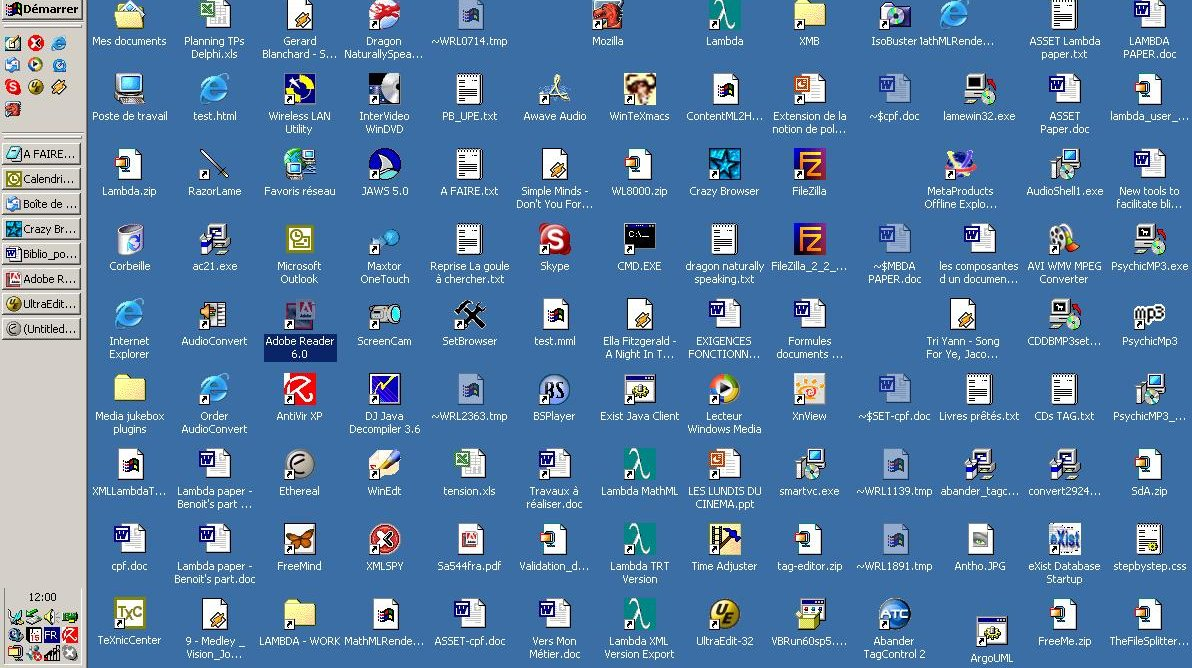
\includegraphics{img/ecran.jpg}
\caption{\label{fig:benoit}Voici le bureau encombré de Benoit\ldots{}}
\end{figure}

\hypertarget{protocole-de-test}{%
\section{Protocole de test}\label{protocole-de-test}}

\hypertarget{sujets}{%
\subsection{Sujets}\label{sujets}}

Neuf sujets volontaires (8 hommes et 1 femme, âgés de 21 ans à 40 ans) ont
participé au test. Tous les sujets sont familiers avec l'utilisation d'une
souris; deux d'entre eux avait déjà utilisé une souris à retour de force.

\hypertarget{matuxe9riel}{%
\subsection{Matériel}\label{matuxe9riel}}

Nous utilisons la souris à retour de force Wingman Force Feedback Mouse
(Figure \ref{fig:wingman}) conçue par (\protect\hyperlink{ref-ImmersionCorporation2005}{{``Immersion corporation,''} n.d.}) et
commercialisée par Logitech.

La manipulation d'un périphérique de pointage à retour de force, comme
notre souris, est basée sur la perception kinesthésique du bras, de la main
et des doigts. La perception cutanée n'est que peu stimulée dans cette
interaction. En d'autres mots, ici, il ne s'agit pas de ressentir une
texture.

L' ordinateur utilisé est un PC 1GHz. Les données ont été collectées par
le serveur (Apache 2 tournant sur un PC à 733 Mhz) sous forme de feuilles de
calcul. Les sujets sont accompagnés par un expérimentateur durant toute la
durée du test.

\hypertarget{procuxe9dure}{%
\subsection{Procédure}\label{procuxe9dure}}

Pendant l'expérience, chaque sujet doit aller cliquer sur un petit rond en
haut à droite de l'écran~: l'origine. Une fois le clic effectué sur l'origine,
une cible hexagonale apparaît à l'écran. Il lui faut aller cliquer le plus
vite possible sur cette cible. Le sujet peut préparer son geste aussi
longtemps qu'il le souhaite, tant que le curseur de la souris ne quitte pas
l'origine. Quand il a cliqué sur la cible, celle-ci disparaît et il doit
retourner à l'origine afin de générer une nouvelle cible.

L'ensemble de l'expérience est divisée en 4 phases, correspondants à 4
conditions de retour haptique~:

\begin{itemize}
\tightlist
\item
  condition MT~: aucun retour de force.
\item
  condition MTF~: un champs de force se déclenche quand
  le curseur de la souris passe au dessus de la cible. À ce moment, la souris
  est attirée au centre de la cible.
\item
  condition MTDF~: l'ensemble de l'écran est une
  mosaïque hexagonale. Lorsqu'il est survolé par le curseur, chaque hexagone
  déclenche un champs de force attirant le périphérique en son centre.
\item
  condition MTDFH~: même chose que la condition MTDF,
  mais l'intensité du retour de force dépend de la vitesse de la souris selon
  la loi
  \[
  Intensit\acute{e}=\frac{Intensit\acute{e}\_{max}}{vitesse+1}\]
\end{itemize}

L'intensité sera ainsi plus faible lorsque la vitesse de la
souris est élevée (voir figure \ref{fig:intensite}).

\begin{figure}
\centering
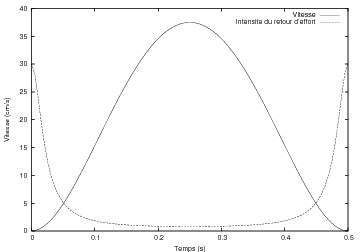
\includegraphics{img/entensite.png}
\caption{\label{fig:intensite}Dans la condition MTDFH, l'intensité du retour de force
dépend de la vitesse du pointeur. Dans le cas idéal d'une trajectoire
minimisant le jerk (voir \ref{jerk}), on aurait le résultat ci-dessus.
Avant chaque phase chronométrée, une phase d'entraînement permet au sujet de
s'habituer à manipuler le périphérique dans les différentes
conditions.}
\end{figure}

Il y a 10 cibles différentes. Chacune est présentée 4 fois au sujet par
phase. Ainsi, chaque sujet aura 160 mouvements origine-cible à réaliser pour
un ensemble de 1440 mouvements pour l'ensemble des sujets.

Les paramètres de l'expérience sont résumés dans la table~\protect\hyperlink{table1}{3.1}.

\begin{longtable}[]{@{}
  >{\raggedright\arraybackslash}p{(\columnwidth - 2\tabcolsep) * \real{0.3333}}
  >{\raggedright\arraybackslash}p{(\columnwidth - 2\tabcolsep) * \real{0.6667}}@{}}
\toprule()
\endhead
DISTANCES À LA CIBLE & 21, 72, 92, 138, 205, 233, 415, 586, 831, 938 pixels \\
TAILLE DE LA CIBLE & 40 pixels \\
CONDITIONS EXPERIMENTALES & * MT~: sans retour de force, \\
& * MTF~: retour de force sur la cible, \\
& * MTDF~ retour de force sur le damier, \\
& * MTDFH~: retour de force adaptatif sur le damier \\
\bottomrule()
\end{longtable}

Table 3.1~: paramètres de
l'expérience.

Ces conditions forment un ensemble homogène de tâches de pointage. Dans ce
protocole de test, nous utilisons la formulation de l'indice de difficulté de
la tâche proposée par MacKenzie {[}MacKenzie (\protect\hyperlink{ref-mackenzie1992fitts}{1992})~:

\begin{equation}
 ID=\log_{2}(A/W+1)
 (#eq:mackenzieID)
\end{equation}

où \(A\) est la distance à la cible, et
\(W\) la taille de la cible (en l'occurrence sa
largeur). En utilisant l'équation \eqref{eq:mackenzieID}, nous
obtenons des indices de difficultés compris entre~:

\[
ID\_{min}=\log_{2}\left(\frac{21}{40}+1\right)=0.61bits\]

et

\[
ID=\log_{2}\left(\frac{938}{40}+1\right)=4.61bits\]

Au final, l'interface de l'expérimentation est présentée sur la
figure \ref{fig:protocole}. (nous noterons que le choix de
l'interface provient de nos recherches sur la représentation instantanée de
la musique, voir la section \protect\hyperlink{application-uxe0-la-musique-musichaptic}{Application à la musique~: Music'Haptic}.

\begin{figure}
\centering
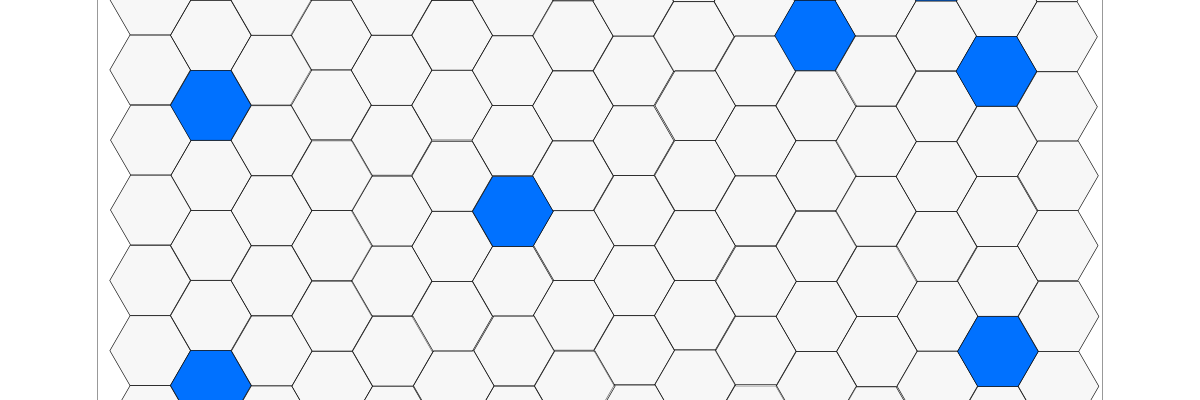
\includegraphics{img/damier.svg}
\caption{\label{fig:protocole}Origine et cibles du protocole\#\# Résultats et discussion}
\end{figure}

L'analyse de la variance (ANOVA) sur les temps de pointage, permet de nous
prononcer sur la significativité des facteurs jouant sur nos mesures~: les
différentes conditions expérimentales et l'indice de difficulté. Il apparaît
que le facteur conditions expérimentales est très significatif
(\emph{F}9,39=24.96, \emph{p}\textless0.0001), ainsi que le facteur indice de difficulté
(\emph{F}3,39=10.3, \emph{p}\textless0.0001). De plus, les deux facteurs n'influent pas l'un
sur l'autre (\emph{F}27,39=0.35, \emph{p}=1.0000).

Les moyennes des temps pour les 4 conditions de retour haptique sont dans
le tableau~\protect\hyperlink{table3}{3.2}.

\begin{longtable}[]{@{}llll@{}}
\toprule()
MT & MTF & MTDF & MTDFH \\
\midrule()
\endhead
585 ms & 584 ms & 723 ms & 676 ms \\
- & (−0,2\%) & (+23,6\%) & (+15,6\%) \\
\bottomrule()
\end{longtable}

Table 3.2~: Moyennes des temps des
mouvements dans les 4 conditions; les pourcentages donnent l'écart
par rapport à la condition MT

Nous pouvons déjà observer qu'il n'y a pas de différence significative
entre cliquer sur une cible sans retour de force (MT) et avec retour de force
(MTF). Ceci rejoint les observations de Akamatsu (\protect\hyperlink{ref-akamatsu1996movement}{Akamatsu and MacKenzie, 1996}) et
s'explique par le fait que le retour de force sur la cible n'est activé que
lorsque le pointeur s'y trouve, à la différence d'autres expériences qui
élargissaient le bassin d'attraction au delà de la taille de la cible
(\protect\hyperlink{ref-hasser1998user}{Hasser et al., 1998}) (\protect\hyperlink{ref-eberhardt1997force}{Eberhardt et al., 1997}) (\protect\hyperlink{ref-wall2000quantification}{Wall and Harwin, 2000}). Par
contre, le fait qu'il y ait des champs de force entre l'origine et la cible
(MTDF et MTDFH) génère une hausse significative des temps (respectivement
+23,6\% et +15,6\% par rapport au mouvement sans retour de force). Enfin,
l'adaptation du retour de force sur la vitesse du curseur permet de réduire
cette perte de performance de 6,5\% .

Nous aurions pu espérer une amélioration plus nette des temps de pointage
dans la condition MTDFH. Cependant, \protect\hyperlink{le-moduxe8le-dimpulsion-initiale}{Le modèle d'impulsion initiale} nous
apporte une explication possible~: Le geste le plus fréquent lors d'une tâche
d'acquisition de cible consiste en un premier mouvement initial qui peut
dépasser ou ne pas atteindre la cible, suivi de plus petits mouvements
correctifs pour parvenir réellement sur la cible. Avec notre retour de force
adaptatif, le geste de pointage pouvait se retrouver «~emprisonné~» sur une
zone proche de la cible.

Les régressions linéaires sur les moyennes des données nous donnent les
coefficients de régression linéaire de l'équation \eqref{eq:mackenzieID} pour
les différentes conditions de retour haptique. Ainsi, la table~\protect\hyperlink{table2}{3.3}
présente les différents modèles de la loi de Fitts selon ces conditions.
Chaque modèle a été calculé en effectuant une régression linéaire entre les
10 indices de difficulté (\emph{ID}), calculé en utilisant l'équation
\eqref{eq:mackenzieID}, et les temps observés.

\begin{longtable}[]{@{}lll@{}}
\toprule()
\endhead
Conditions & Modèle de la loi de Fitts & \(R^2\) \\
MT & \(MT=0,25+0,122ID\) & 0,93 \\
MTF & \(MT=0,25+0,120ID\) & 0,91 \\
MTDF & \(MT=0,38+0,123ID\) & 0,96 \\
MTDFH & \(M*=0,31+0,130ID\) & 0,90 \\
\bottomrule()
\end{longtable}

Table 3.3~: Modèles de la loi de Fitts.
MT est le temps du mouvement(ms), ID est l'indice de
difficulté(bits)

Les différentes conditions ne diffèrent de manière significative que de
par leurs ordonnées à l'origine. Les pentes de chaque modèle sont très
proches. Enfin, nous pouvons noter, grâce aux valeurs élevées des
\emph{R}² que la loi de Fitts explique plus de 90\% des
variations dans les observations.

Nous pouvons maintenant tracer la synthèse des mesures de notre expérience
(figure \ref{fig:synthese}).

\begin{figure}
\centering
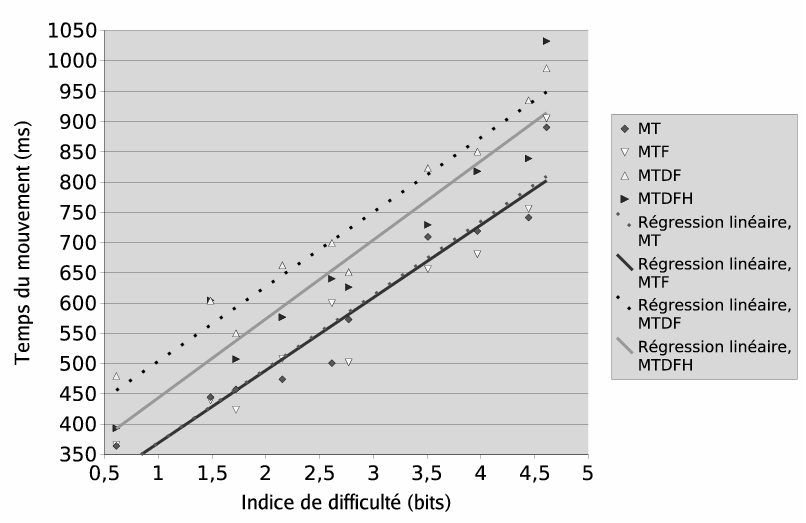
\includegraphics{img/synth.png}
\caption{\label{fig:synthese}Temps du mouvement pour les 4 conditions de retour
haptique}
\end{figure}

La méthode statistique de Bonferroni permet de grouper les observations en
groupes significativement différents. Dans notre cas, cette méthode regroupe
les observations MT et MTF en un premier groupe non-significativement
différent, et les conditions MTDF et MTDFH en un deuxième. Notre proposition
d'adapter le retour haptique à la vitesse de la souris (condition MTDFH)
n'apparaît donc pas significativement différent de la condition sans
adaptation (\emph{p}\textgreater0.15).

\hypertarget{conclusion-2}{%
\section{Conclusion}\label{conclusion-2}}

Il est donc apparu que le retour de force pouvait améliorer les
performances, mais dans des cas peu applicables à des situations complexes~:
une seule cible haptiquement augmentée. Dans le cas d'une multiplication des
cibles potentielles, le retour haptique devient même un facteur de perte de
performances. Dans notre cas, les temps de pointage ont augmenté de 23\%
lorsque l'écran est compétement rempli de distracteurs haptiques.

Nous avons proposé ici un retour de force adaptatif, calculé en fonction
de la vitesse courante du pointeur. Les performances s'améliorent alors de
6,5\%.

Pour aller plus loin, nous pouvons imaginer tester d'autres adaptation
dynamiques des forces, basées sur l'accélération du curseur, par exemple. De
plus, nous pourrions tester des zones d'attirance englobant plusieurs cibles,
et ce, de manière à éviter au curseur de tomber dans une mauvaise cible.

Notons que dans un contexte d'accessibilité, l'intérêt de l'utilisation de
dispositifs à retour de force a déjà été prouvé, par exemple auprès de
personnes handicapés moteurs (\protect\hyperlink{ref-keates2002use}{Keates et al., 2002}).

Au final, cette étude nous a permis d'étudier la partie action du mode
haptique, et plus précisément \protect\hyperlink{duxe9finitions}{les gestes \textbf{déictiques}}
(\protect\hyperlink{ref-McNeill92}{McNeill, 1992}). Dans tout ce chapitre, en effet, il s'agissait
d'utiliser une souris à retour de force dans un registre classique pour une
souris~: le pointage. Le retour de force essayant d'améliorer la vitesse de
pointage.

Dans la seconde partie de cette thèse, nous allons passer aux gestes
\textbf{épistémiques} de (\protect\hyperlink{ref-cadoz1994realites}{Cadoz, 1994}),
c'est à dire aux gestes effectués pour prendre des connaissance du monde
extérieur. Ce sont ces gestes, et leurs retours de forces associés, qui vont
nous permettre d'envisager une utilisation de la modalité haptique, dans un
but d'accessibilité des personnes non-voyantes aux documents numériques.

\hypertarget{part-haptique-et-accessibilituxe9}{%
\part{Haptique et Accessibilité}\label{part-haptique-et-accessibilituxe9}}

\hypertarget{vers-laccessibilituxe9}{%
\chapter{Vers l'accessibilité}\label{vers-laccessibilituxe9}}

\hypertarget{introduction-3}{%
\section{Introduction}\label{introduction-3}}

Avec les interfaces graphiques à manipulation
directe (GUIs), l'utilisateur interagit avec l'ordinateur à l'aide
d'un écran, d'un dispositif de pointage - en général une souris -
et d'un clavier. Ces interfaces sont dites faciles à apprendre et à
utiliser, grâce à une spatialisation de l'information qui réduit la
charge cognitive de l'utilisateur. Toutefois, ce schéma
d'interaction est incomplet~: il exclut les utilisateurs
non-voyants.

Dans ce chapitre, nous allons tâcher de synthétiser ce que la littérature
nous indique quant à l'accès des non-voyants aux systèmes interactifs, tout
d'abord dans un cadre général; puis dans un contexte d'utilisation du système
haptique.

\hypertarget{linteraction-non-visuelle}{%
\section{L'interaction non-visuelle}\label{linteraction-non-visuelle}}

\hypertarget{duxe9finitions-du-handicap}{%
\subsection{Définitions du handicap}\label{duxe9finitions-du-handicap}}

La déclaration des droits des personnes handicapées proclamée par
l'assemblée générale de l'Organisation des Nations Unies le 9 décembre 1975
indique que «~toute personne dans l'incapacité d'assurer par elle-même tout
ou partie des nécessités d'une vie individuelle ou sociale normale, du fait
d'une déficience, congénitale ou non, de ses capacités physiques ou mentales~»
est une personne handicapée.

En 1980, l'organisation Mondiale de la Santé (\protect\hyperlink{ref-world1980international}{Organization et al., 1980}), dans
le rapport du rhumatologue britannique, Philip WOOD, introduit une
clarification conceptuelle dans la définition du handicap, reprise en France
sous le titre de '' Classification internationale des handicaps (CIH)~:
déficiences, incapacités, désavantages. Il y est défini le handicap comme
la conséquence des maladies sur la personne suivant trois plans~:

\begin{itemize}
\item
  \textbf{la déficience}, correspondant à l'altération
  d'une structure ou d'une fonction psychologique, physiologique ou
  anatomique. La déficience peut-être temporaire ou définitive;
\item
  \textbf{l'incapacité}, qui est une réduction partielle
  ou totale de la capacité d'accomplir de façon normale une activité.
  L'incapacité est en quelque sorte la conséquence fonctionnelle de la
  déficience mais elle ne dépend pas obligatoirement de celle-ci. D'autre
  part, une déficience peut très bien ne s'accompagner d'aucune
  incapacité;
\item
  \textbf{le désavantage} ou \textbf{le handicap},
  conséquence de la déficience ou de l'incapacité sur les conditions
  d'insertion sociale, scolaire ou professionnelle.
\end{itemize}

Dans l'union européenne, c'est près d'un tiers de la population qui
souffre de troubles divers (voir le tableau \ref{tab:population}).

\begin{longtable}[]{@{}
  >{\raggedright\arraybackslash}p{(\columnwidth - 6\tabcolsep) * \real{0.2268}}
  >{\raggedright\arraybackslash}p{(\columnwidth - 6\tabcolsep) * \real{0.2680}}
  >{\raggedright\arraybackslash}p{(\columnwidth - 6\tabcolsep) * \real{0.2990}}
  >{\raggedright\arraybackslash}p{(\columnwidth - 6\tabcolsep) * \real{0.2062}}@{}}
\caption{\label{tab:population} Population souffrant de troubles
dans les états membres de l'Union Européenne (adapté de {[}TIDE 96{]}).}\tabularnewline
\toprule()
\begin{minipage}[b]{\linewidth}\raggedright
Type de troubles
\end{minipage} & \begin{minipage}[b]{\linewidth}\raggedright
Estimation (en millions)
\end{minipage} & \begin{minipage}[b]{\linewidth}\raggedright
\% des personnes handicapées
\end{minipage} & \begin{minipage}[b]{\linewidth}\raggedright
\% de la population
\end{minipage} \\
\midrule()
\endfirsthead
\toprule()
\begin{minipage}[b]{\linewidth}\raggedright
Type de troubles
\end{minipage} & \begin{minipage}[b]{\linewidth}\raggedright
Estimation (en millions)
\end{minipage} & \begin{minipage}[b]{\linewidth}\raggedright
\% des personnes handicapées
\end{minipage} & \begin{minipage}[b]{\linewidth}\raggedright
\% de la population
\end{minipage} \\
\midrule()
\endhead
Physique & 24.80 & 68\% & 7.7\% \\
Visuel & 6.50 & 15.80\% & 2\% \\
Auditif & 8.70 & 23.90\% & 2.7\% \\
Mental & 7.40 & 20.30\% & 2.3\% \\
Communication verbal & 3.60 & 10\% & 1.1\% \\
\bottomrule()
\end{longtable}

Le tableau \ref{tab:malvoyants} montre les
statistiques sur les populations mal-voyantes et non-voyantes. En France, sur
18000 aveugles en âge de travailler, environ 6000 travaillent, dont 1500
manuels (les 2/3 en secteur protégé), 1500 standardistes, 1300 masseurs
kinésithérapeutes, 600 enseignants (en milieu spécialisé ou ordinaire), 400
sténodactylos, 300 musiciens professionnels, 300 divers (juristes, cadres de
la fonction publique, informaticiens); plus de 50\% ne peuvent trouver du
travail. {[}Quid 2005{]}

\begin{longtable}[]{@{}
  >{\raggedright\arraybackslash}p{(\columnwidth - 4\tabcolsep) * \real{0.4167}}
  >{\raggedright\arraybackslash}p{(\columnwidth - 4\tabcolsep) * \real{0.2500}}
  >{\raggedright\arraybackslash}p{(\columnwidth - 4\tabcolsep) * \real{0.3333}}@{}}
\caption{\label{tab:malvoyants} Populations non et mal-voyantes en France et dans le monde}\tabularnewline
\toprule()
\begin{minipage}[b]{\linewidth}\raggedright
\end{minipage} & \begin{minipage}[b]{\linewidth}\raggedright
Troubles visuels
\end{minipage} & \begin{minipage}[b]{\linewidth}\raggedright
Aveugles + mal-voyants
\end{minipage} \\
\midrule()
\endfirsthead
\toprule()
\begin{minipage}[b]{\linewidth}\raggedright
\end{minipage} & \begin{minipage}[b]{\linewidth}\raggedright
Troubles visuels
\end{minipage} & \begin{minipage}[b]{\linewidth}\raggedright
Aveugles + mal-voyants
\end{minipage} \\
\midrule()
\endhead
Monde (OMS février 2000) & 160~000~000 & 45~000~000 \\
France (1997) & 1~500~000 & 110~000~+~250~000 \\
\% de la population française & 2.6\% & \\
\bottomrule()
\end{longtable}

Enfin, la France a voté le 12 février 2005 la loi n°102-2005 pour
l'égalité des droits et des chances, la participation et la citoyenneté des
personnes handicapées, dont l'article 47 rend obligatoire l'accessibilité des
sites Web du secteur public.

\hypertarget{les-capacituxe9s-sensorielles-chez-les-non-voyants}{%
\subsection{Les capacités sensorielles chez les non-voyants}\label{les-capacituxe9s-sensorielles-chez-les-non-voyants}}

(\protect\hyperlink{ref-grant2000tactile}{Grant et al., 2000}) ont conduit
une étude sur des personnes non-voyantes et voyantes. Il s'agissait
d'apprécier la précision de la perception tactile des deux populations, et
établir un éventuel lien entre le handicap et les capacités sensorielles. En
fin de compte, cette étude a prouvé que les non-voyants obtenaient de
meilleurs résultats que les voyants au début des tests, mais que cet avantage
diminuait au fur et à mesure, jusqu'à disparaître.

En fait, il a été souvent dit que les aveugles développaient des capacités
sensorielles supra-normales, telles que l'acuité auditive, ou somesthésique.
Dans la pratique, cependant, il a été prouvé que l'acuité haptique
(\protect\hyperlink{ref-heller1989texture}{Heller, 1989}) était équivalente chez les
non-voyants congénitaux, chez les non-voyants accidentels et chez les
personnes voyantes.

\hypertarget{la-repruxe9sentation-mentale-dun-document-par-une-personne-non-voyante}{%
\subsection{La représentation mentale d'un document par une personne non-voyante}\label{la-repruxe9sentation-mentale-dun-document-par-une-personne-non-voyante}}

Une personne aveugle se sert énormément de sa mémoire et relativement peu
de ses sens, alors que l'activité d'une personne voyante est essentiellement
basée sur la vue et la coordination oeil-main.

Pourtant, les travaux de (\protect\hyperlink{ref-hatwell1993images}{Hatwell, 1993}) et de (\protect\hyperlink{ref-martial1998representation}{Martial, 1998})
ont montré que la représentation mentale des non-voyants est identique à celle
des voyants. En effet, même si l'on parle habituellement de mémoire visuelle,
lorsque l'on considère la représentation mentale de quelque chose, tout est
basé sur l'expérience de l'espace. En d'autres mots, pour se construire une
représentation mentale de ce qui leur est décrit, une personne aveugle
s'appuiera sur les notions qu'il a de l'espace~: en haut, à droite, à l'est,
derrière.

Dans une autre expérience, (\protect\hyperlink{ref-manghi2003composantes}{Manghi, 2003}) a demandé à ses sujets
(l'étude portait sur des voyants et des non-voyants, et explorait également les
effets de l'âge) de décrire un trajet dans une ville à quelqu'un. Les résultats
se sont révélés très intéressants~:

\begin{enumerate}
\def\labelenumi{\arabic{enumi}.}
\tightlist
\item
  Les personnes non-voyantes ont obtenu des
  résultats équivalent quant au taux de réussite de la tâche,
\item
  Leurs descriptions d'itinéraires ont été surtout
  jugées plus pertinent, avec notamment l'utilisation

  \begin{itemize}
  \tightlist
  \item
    de repère absolus (le nord, le banc sur le
    trottoir\ldots)
  \item
    de précisions dans les mesures (angles,
    distances),
  \item
    de repères multimodaux (le carrefour, le
    marteau-piqueur\ldots)
  \end{itemize}
\end{enumerate}

Il y a cependant, entre un voyant et un non-voyant, une différence très
importante, lors de l'accès aux documents textuels~: le non voyant ne peut pas
se faire une idée globale de la forme du texte. Inversement, lors d'une tâche
de lecture, une personne voyante peut parcourir l'ensemble du document très
rapidement, et par exemple, repérer rapidement l'item qui l'intéresse.

Pour se faire une idée assez rapide du texte avant la lecture, les
non-voyants utilisent une synthèse vocale réglée sur un débit rapide.
Cependant, la mémoire auditive demande une grande concentration. Ainsi,
l'utilisation d'une autre modalité, comme le toucher, peut permettre de
réduire la charge mentale.

En conclusion, un non-voyant se construit une image mentale identique en
tout point à celle d'une personne voyante. Cependant, la construction d'une
telle représentation mentale nécessite une description de la disposition
globale, ou des mécanismes de navigation dans le document. Enfin, on pourra
s'appuyer sur une grande précision dans les descriptions.

\hypertarget{modalituxe9s-non-visuelles-disponibles-en-sortie}{%
\subsection{Modalités non-visuelles disponibles en sortie}\label{modalituxe9s-non-visuelles-disponibles-en-sortie}}

Contrairement à ceux de l'être humain, les médias non visuels en sortie
restent limités (tableau \ref{tab:media-non-visuels}).
Les systèmes basés sur les sens de l'odorat et du goût restent très rares.
Maintenant, les périphériques de pointage à retour d'effort se démocratisent
de plus en plus (voir \href{016-les-peripheriques-de-sortie-a-retour-haptique.html}{2.5}).

\begin{longtable}[]{@{}
  >{\raggedright\arraybackslash}p{(\columnwidth - 6\tabcolsep) * \real{0.1558}}
  >{\raggedright\arraybackslash}p{(\columnwidth - 6\tabcolsep) * \real{0.4286}}
  >{\raggedright\arraybackslash}p{(\columnwidth - 6\tabcolsep) * \real{0.2143}}
  >{\raggedright\arraybackslash}p{(\columnwidth - 6\tabcolsep) * \real{0.2013}}@{}}
\caption{\label{tab:media-non-visuels}Sens perceptifs humain et médias informatiques
(adapté de (\protect\hyperlink{ref-truillet1999modelisation}{Truillet, 1999}))}\tabularnewline
\toprule()
\begin{minipage}[b]{\linewidth}\raggedright
Sens perceptifs humain
\end{minipage} & \begin{minipage}[b]{\linewidth}\raggedright
Médias informatiques
\end{minipage} & \begin{minipage}[b]{\linewidth}\raggedright
Stimuli
\end{minipage} & \begin{minipage}[b]{\linewidth}\raggedright
Récepteurs
\end{minipage} \\
\midrule()
\endfirsthead
\toprule()
\begin{minipage}[b]{\linewidth}\raggedright
Sens perceptifs humain
\end{minipage} & \begin{minipage}[b]{\linewidth}\raggedright
Médias informatiques
\end{minipage} & \begin{minipage}[b]{\linewidth}\raggedright
Stimuli
\end{minipage} & \begin{minipage}[b]{\linewidth}\raggedright
Récepteurs
\end{minipage} \\
\midrule()
\endhead
Ouïe & Haut-parleurs, casque audio & Parole, bruit, son & Oreilles \\
Haptique & Afficheur braille, sondes chauffantes, système à retour de force & Texture, température, mouvement & Peau, Muscles, tendons, corps \\
Odorat & ? & Odeurs & Nez \\
Goût & ? & Saveur & Langue \\
\bottomrule()
\end{longtable}

\hypertarget{utilisation-et-justification-de-la-multimodalituxe9}{%
\subsection{Utilisation et justification de la multimodalité}\label{utilisation-et-justification-de-la-multimodalituxe9}}

(\protect\hyperlink{ref-dufresne1995multimodal}{Dufresne et al., 1995}) ont montré
l'impact et l'intérêt de la bimodalité audio-haptique pour les utilisateurs
non-voyants. Le tableau \ref{tab:modalite} indique le
pourcentage de bonnes réponses dans trois situations modales; pour 12 voyants
et 12 non-voyants. Il est à noter que dans cette expérience, les sujets
non-voyants ont obtenus de meilleurs scores~: leur concentration était
supérieure.

\begin{longtable}[]{@{}
  >{\raggedright\arraybackslash}p{(\columnwidth - 6\tabcolsep) * \real{0.2250}}
  >{\raggedright\arraybackslash}p{(\columnwidth - 6\tabcolsep) * \real{0.3375}}
  >{\raggedright\arraybackslash}p{(\columnwidth - 6\tabcolsep) * \real{0.2875}}
  >{\raggedright\arraybackslash}p{(\columnwidth - 6\tabcolsep) * \real{0.1500}}@{}}
\caption{\label{tab:modalite} Bonnes réponses dans différentes situations modales}\tabularnewline
\toprule()
\begin{minipage}[b]{\linewidth}\raggedright
Modalité
\end{minipage} & \begin{minipage}[b]{\linewidth}\raggedright
Testeurs non-voyants~: 12
\end{minipage} & \begin{minipage}[b]{\linewidth}\raggedright
Testeurs voyants~: 12
\end{minipage} & \begin{minipage}[b]{\linewidth}\raggedright
Total~: 24
\end{minipage} \\
\midrule()
\endfirsthead
\toprule()
\begin{minipage}[b]{\linewidth}\raggedright
Modalité
\end{minipage} & \begin{minipage}[b]{\linewidth}\raggedright
Testeurs non-voyants~: 12
\end{minipage} & \begin{minipage}[b]{\linewidth}\raggedright
Testeurs voyants~: 12
\end{minipage} & \begin{minipage}[b]{\linewidth}\raggedright
Total~: 24
\end{minipage} \\
\midrule()
\endhead
Audio & 68\% & 62\% & 64\% \\
Haptique & 78\% & 71\% & 74\% \\
Audio + haptique & 83\% & 78\% & 80\% \\
Total & 76\% & 70\% & 73\% \\
\bottomrule()
\end{longtable}

\hypertarget{laccessibilituxe9-duxe9finitions}{%
\section{L'accessibilité : définitions}\label{laccessibilituxe9-duxe9finitions}}

\begin{quote}
The power of the Web is in its universality. Access by everyone regardless of
disability is an essential aspect.

Tim Berners-Lee, l'inventeur du World Wide Web
\end{quote}

\hypertarget{laccessibilituxe9-par-tim-berners-lee-directeur-du-w3c-et-inventeur-du-world-wide-web}{%
\subsection{L'accessibilité par Tim Berners-Lee, directeur du W3C et inventeur du World Wide Web}\label{laccessibilituxe9-par-tim-berners-lee-directeur-du-w3c-et-inventeur-du-world-wide-web}}

\begin{quote}
Mettre le Web et ses services à la disposition de tous les individus, quel
que soit leur matériel ou logiciel, leur infrastructure réseau, leur langue
maternelle, leur culture, leur localisation géographique, ou leurs
aptitudes physiques ou mentales.

L'accès à l'information et à la communication est un droit universel. Le
web est devenu un média majeur, et il se doit d'être accessible à tous sans
discrimination. Concevoir dans le cadre du design for all (conception pour
tous), c'est anticiper sur les usages, répondre à une logique de
développement durable et surtout, utiliser la technologie dans le respect
des individualités.
\end{quote}

\hypertarget{laccessibilituxe9-par-denis-chuxeane-france-tuxe9luxe9com-rd}{%
\subsection{L'accessibilité par Denis Chêne, France-Télécom R\&D}\label{laccessibilituxe9-par-denis-chuxeane-france-tuxe9luxe9com-rd}}

\begin{quote}
Être accessible c'est avant tout permettre l'accès. L'accès aux
informations (documents, nouvelles, bases de données) ; l'accès aux
échanges, qu'il s'agisse des échanges en terme de communication (audio,
vidéo, texte\ldots) ou des échanges de biens de consommation (achats divers,
gestion monétaire\ldots).

Mais, être accessible c'est aussi permettre l'utilisation, car rien ne
sert d'accéder si l'on ne peut utiliser. Consulter , c'est bien, mais faire
, c'est mieux.

La richesse du numérique, c'est sa malléabilité. La malléabilité permet
en effet de reformuler les données échangées de façon à correspondre à
chaque type d'utilisateur et de situations. Il existe en effet de nombreux
types d'utilisateurs différents, qui accèdent à l'information de façons
diverses, selon des contextes variés (absence de visibilité, d'audition, de
motricité, de compréhension). Rendre l'information et les échanges
accessibles, c'est optimiser, pour chaque individu, pour chaque contexte
d'usage, l'acquisition, la production, et la manipulation d'informations et
d'éléments pouvant être atteints sur ou via le web.

La richesse du web c'est son gigantisme. D'aucun diront qu'il est
impossible, sur une telle masse, de gérer toutes les individualités et tous
les contextes, et que 'faire du spécifique' est coûteux et peu rentable.
Certes, mais l'objet n'est justement pas de faire du spécifique, mais du
générique qui puisse servir à tous, sans exception. Ce faisant,
l'accessibilité est moins coûteuse~: l'araignée gagnera à tisser une toile
solide plutôt qu'une toile fragile aux nombreuses rustines ; et plus
rentable~: davantage d'utilisateurs pourront y accéder dans plus de
contextes d'usages.

Au final, l'accessibilité résulte d'une conception pour tous . Or, la
richesse de l'être humain, c'est sa diversité.
\end{quote}

\hypertarget{la-web-accessibility-initiative-wai-du-world-wide-web-consortium-w3c}{%
\subsection{\texorpdfstring{La \emph{Web Accessibility Initiative} (WAI) du \emph{World Wide Web Consortium} (W3C)}{La Web Accessibility Initiative (WAI) du World Wide Web Consortium (W3C)}}\label{la-web-accessibility-initiative-wai-du-world-wide-web-consortium-w3c}}

Le \emph{World Wide Web Consortium}, abrégé W3C\footnote{\url{http://www.w3.org}}, est
un consortium fondé en octobre 1994 pour promouvoir la compatibilité des
technologies du \emph{World Wide Web} telles que HTML, XHTML, XML, CSS,
PNG, SVG et SOAP. Le W3C n'émet pas des normes, mais des recommandations.

Le consortium laisse le soin aux fabricants de suivre les recommandations.
Contrairement à l'Organisation internationale de normalisation ou d'autres
corps internationaux de standardisation, le W3C ne possède pas de programme
de certification, et beaucoup de standards ne définissent pas formellement un
niveau de conformité. Ils sont ainsi souvent implantés partiellement.

Concernant l'accessibilité, le W3C a créé des recommandations à travers le
projet WAI (\emph{Web Accessibility Initiative}) en 1996. Ces
recommandations s'adressent à tous les distributeurs de contenu numérique par
Internet~: navigateurs, documents HTML, logiciels d'édition de HTML, logiciel
du publication de site Web créant le code HTML.

Les recommandations de la WAI actuellement en vigueur sont~:

\begin{itemize}
\tightlist
\item
  les \emph{Authoring Tool Accessibility Guidelines}
  (ATAG) qui posent les règles d'accessibilité pour les outils
  d'édition.
\item
  les \emph{Web Content Accessibility Guidelines}
  (WCAG) qui montrent comment créer des documents Web avec un contenu
  accessible aux utilisateurs souffrant de handicaps.
\item
  les \emph{User Agent Accessibility Guidelines}
  (UAAG), enfin, posent les règles pour l'accessibilité des agents
  utilisateurs.
\end{itemize}

On pourra se référer aux \protect\hyperlink{accessibilite}{annexes}, pour plus de détails.

\hypertarget{autres-aspects-de-laccessibilituxe9}{%
\subsection{Autres aspects de l'accessibilité}\label{autres-aspects-de-laccessibilituxe9}}

\begin{quote}
L'accessibilité n'est pas une fonctionnalité, mais bien un processus (une
méthode) que l'on intègre tout au long du cycle de vie d'un projet.

Pierre Guillou (responsable de la cellule accessibilité de l'association
BrailleNet)
\end{quote}

\hypertarget{accessibilituxe9-notre-positionnement}{%
\subsection{Accessibilité: notre positionnement}\label{accessibilituxe9-notre-positionnement}}

\begin{quote}
Nous nous positionnons pour une accessibilité au
sens large. Il s'agit d'une approche visant à étendre la démarche
d'accessibilité au delà d'un public spécifique. En employant
l'illustration du \textless{}\textgreater,
concevoir un site Web accessible pour une personne non-voyante, rendra ce
site Web plus simple d'usage pour l'ensemble des utilisateurs. La
problématique de cette thèse traite de l'utilisation de dispositifs à
retour de force en matière d'accessibilité, à priori pour les personnes
souffrant d'handicap visuel; maintenant, quand nous proposerons des
solutions techniques utilisables spécifiquement par des personnes
handicapées, les concepts utilisés, et les solutions techniques retenus
peuvent (et doivent) être reprises dans des contextes plus larges; dans
des situations où le sens de la vue serait mobilisé sur une autre tâche,
par exemple.
\end{quote}

Nous allons cependant passer en revue ce qui a déjà été réalisé
spécifiquement pour des personnes souffrant d'un handicap visuel, en matière
d'accessibilité, et mettant en œuvre des dispositifs haptiques. Nous
retiendrons que ces approches peuvent être reprises sans public spécifique,
avec une interaction augmentée par le sens haptique.

\hypertarget{laccessibilituxe9-des-personnes-non-voyantes-et-mal-voyantes-gruxe2ce-uxe0-un-dispositif-uxe0-retour-haptiquetitre}{%
\section{L'accessibilité des personnes non-voyantes et mal-voyantes grâce à un dispositif à retour haptiquetitre'')}\label{laccessibilituxe9-des-personnes-non-voyantes-et-mal-voyantes-gruxe2ce-uxe0-un-dispositif-uxe0-retour-haptiquetitre}}

L'idée de base de l'utilisation de périphériques à retour haptique pour
des utilisateurs non-voyants, est de palier, autant que raisonnablement
possible, à l'absence de canal visuel. Dans cette approche, plusieurs
contextes d'utilisation ont été explorés.

Nous allons les étudier plus précisément, afin de dégager des pistes pour
notre propre approche.

\hypertarget{identifier-le-contenu-et-lagencement-dun-document}{%
\subsection{Identifier le contenu et l'agencement d'un document}\label{identifier-le-contenu-et-lagencement-dun-document}}

D. Offen et B. Thomlinson ont développé une librairie de programmation
permettant d'identifier l'agencement d'un document (\protect\hyperlink{ref-offen2001good}{Offen and Thomlinson, 2001}).
L'OPENBook (c'est le nom
de la librairie) est ainsi capable d'identifier les colonnes, les titres, les
blocs de texte, les illustrations, les légendes, les tableaux, les entêtes et
les pieds de pages. Un synthétiseur vocal permet de lire~le contenu du
document. Le périphérique utilisé est la souris Wingman Force Feedback de
Logitech. L'utilisateur pourra alors accéder à l'information de plusieurs
manières~:

\begin{enumerate}
\def\labelenumi{\arabic{enumi}.}
\tightlist
\item
  Le mode «~Page Layout Summary~» (pour
  \emph{résumé de la disposition de la page}) rapportera le nombre
  d'éléments de chaque type visibles sur la page. Par exemple 1 titre, 2
  colonnes, 1 illustration .
\item
  Le mode «~Guided Layout~» (pour
  \emph{disposition guidée}) , l'utilisateur sera passif, et se laissera
  guider (ainsi que sa main avec la souris à retour de force) dans un ordre
  logique dans la lecture du document. Le synthétiseur vocal annonçant le nom
  de chaque élément.
\item
  Avec le mode «~Explore Layout » (pour
  \emph{disposition explorée}), l'utilisateur est actif, et contrôle le
  mouvement d'un élément à un autre, en entendant la synthèse vocale lui dire
  de quoi il s'agit.
\end{enumerate}

\hypertarget{toucher-un-document-graphique}{%
\subsection{Toucher un document graphique}\label{toucher-un-document-graphique}}

C. Ramstein est un des pionniers dans les interfaces utilisateur haptiques
pour des personnes ayant un handicap visuel (\protect\hyperlink{ref-ramstein1996touching}{Ramstein et al., 1996}). Il a été à
la tête de Haptic Technologies Inc.~qui fabriquait et vendait les systèmes de
PenCAT/MouseCAT et de TouchDesktop (c'est la couche logicielle qui gère les
périphériques de Haptic Technologies). Le travail de Ramstein s'appuie sur
des interfaces multimodales. L'information haptique est combinée avec
l'information sonore et l'affichage Braille.

J. P. Fritz et K. E. Barner {[}Department of Electrical and Computer
Engineering at the University of Delaware{]} ont travaillé depuis l'apparition
du PHANTOM, sur un système haptique de visualisation pour des personnes avec
handicap visuel (\protect\hyperlink{ref-fritz1996design}{Fritz and Barner, 1996}) (\protect\hyperlink{ref-fritz1999design}{Fritz and Barner, 1999}). Le cœur du
projet n'est pas basé sur une traduction des interfaces utilisateurs en
information haptique mais sur l'utilisation de formes haptiques virtuelles.
Ainsi, leurs travaux visent à transcrire de l'information non-textuelle,
telle que des figures mathématiques, ou des tableaux contenant des données
scientifiques. Leur approche consiste à générer une forme tridimensionnelle,
et à lui donner une existence haptique grâce au PHANTOM.

Les laboratoires de British-Telecom ont étudié l'utilisation d'un
affichage haptique couplé au VRML (Virtual Reality Markup Language), le
format pour l'affichage des graphiques 3D sur le Web (\protect\hyperlink{ref-hardwick1998tactile}{Hardwick et al., 1998}).
Le travail est basé sur une expérience acquise du développement d'un navigateur
capable de piloter un retour de force à partir d'un fichier VRML. On retrouve
ici l'approche de la bibliothèque de programmation Ghost™SDK de Sensable~: le
dispositif de pointage remplace le doigt de l'utilisateur dans l'espace
virtuel, et permet de toucher les objets.

Dans ces trois premières approches, il s'agit de découvrir un objet
tridimensionnel à l'aide d'un dispositif de pointage à retour de force. On
retrouve ainsi les limitations suivantes issues du
tableau \ref{tab:possibilite}~:

\textbar----------------------\textbar-------------------------------------------------------------\textbar{}
\textbar{} L'enveloppement \textbar{} Non possible en l'absence de plusieurs points de contact \textbar{}
\textbar{} Le suivi de contours \textbar{} Possible, mais très difficile du fait d'une zone de contact \textbar{}

J. A. Gardner et V. Bulatov (\protect\hyperlink{ref-gardner2001smart}{Gardner and Bulatov, 2001}) se sont appuyés sur le format
SVG (Scalable Vector Graphics) qui est le format XML pour les images
vectorielles. Associé à une souris à retour de force et à un retour sonore, des
images peuvent être rendue accessibles, tant qu'elles ne sont pas trop
complexes aux non-voyants. Il s'agissait par exemple de localiser les
positions des différentes régions
sur une carte géographique, grâce au rendu d'une texture particulière et d'un
retour sonore, quand le pointeur de la souris passe au centre d'une chaque
région. Cette approche est très similaire à ce que nous avons réalisé, voir
la section \ref{geogrhaptique}.

Wai Yu, de l'université de Glasgow a beaucoup étudié l'utilisation d'une
souris à retour de force ou du PHANTOM dans les problèmes d'accessibilité. Il
a proposé tout d'abord une méthode permettant aux non-voyants d'accéder à des
graphiques mathématiques à l'aide du PHANTOM (\protect\hyperlink{ref-yu2001haptic}{Yu et al., 2001}). La
figure \ref{fig:haptiquement} est issue de cette application~: lorsqu'il
passe à proximité d'un des segments, le pointeur du dispositif est attiré sur
lui.

\begin{figure}
\centering
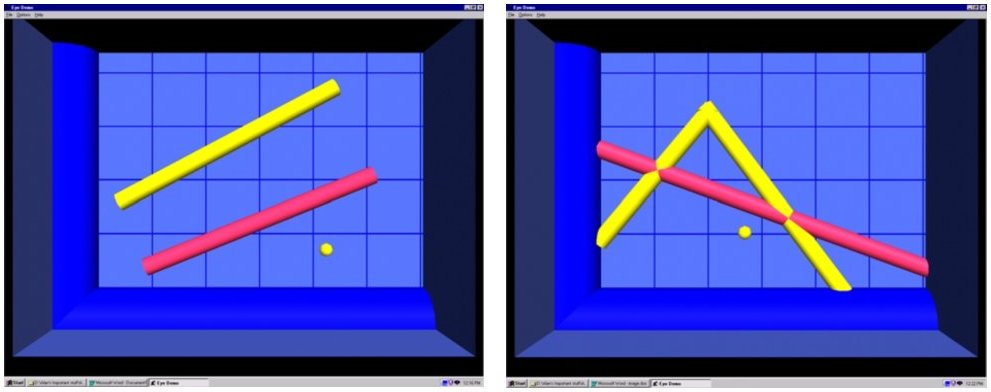
\includegraphics{img/hapticGraphs.jpg}
\caption{\label{fig:haptiquement}Exemples de graphiques haptiquement augmentés}
\end{figure}

Plus tard, il a continué son travail en proposant cette même accessibilité
dans un contexte Web~: l'application tourne dans un navigateur internet et
utilise la souris Wingman Force Feedback. Pour cela il a exploré la
construction automatique de graphiques haptiques (\protect\hyperlink{ref-yu2002automatic}{Yu et al., 2002}), puis, il
a donné à l'utilisateur non-voyant, la possibilité de créer ses propres
graphiques (\protect\hyperlink{ref-yu2003web}{Yu et al., 2003}).

Enfin, (\protect\hyperlink{ref-sjostrom2002non}{Sjostrom, 2002}) a également
étudié le rendu de graphiques mathématiques, mais uniquement à l'aide d'un
PHANTOM. Son approche cherche à être plus proche d'une réelle situation
pédagogique. On peut citer les histogrammes haptiques, obtenus par effet de
cloisonnement, ou les courbes mathém'haptiques , qui comme pour Wai Yu, sont
issues d'un effet d'attirance sur la courbe.

\hypertarget{permettre-dappruxe9hender-les-formes-et-les-textures}{%
\subsection{Permettre d'appréhender les formes et les textures}\label{permettre-dappruxe9hender-les-formes-et-les-textures}}

(\protect\hyperlink{ref-fritz1996design}{Fritz and Barner, 1996}) ont développé une
méthode synthétisant des textures haptiques perceptiblement distinctes en
utilisant des techniques de modélisation stochastiques. Leur but était de
créer un ensemble de textures qui pourraient alors être utilisées pour
décrire des illustrations complexes de données.

Dans ces travaux, les périphériques utilisés sont
\href{\ref{fig:PHANTOM}}{des PHANTOMs}
ou l'Impulse Engine 3000 (figure~\protect\hyperlink{cap:Lux5ctextquotesingleux7bux7dimpulse-engine-3000}{4.2}). En effet,
pour générer des textures
probantes, il est nécessaire d'utiliser du matériel disposant d'une
résolution spatiale très fine~: 0.03mm et 0.01mm respectivement pour le
PHANTOM et l'Impulse Engine 3000.

(\protect\hyperlink{ref-colwell1998haptic}{Colwell et al., 1998}) a étudié la
perception des textures, des formes et des objets virtuels par des sujets
voyants et non-voyants à l'aide de l'Impulse Engine 3000
(figure \ref{fig:impulse}). Ces travaux font partie des grandes références
du domaine (voir les \protect\hyperlink{recommandations-de-conception}{Recommandations de conception}.

\begin{figure}
\centering
\includegraphics{img/impulse.png}
\caption{\label{fig:impulse}L'impulse engine 3000}
\end{figure}

Enfin, (\protect\hyperlink{ref-sjostrom2001designing}{Sjostrom, 2001}) a étudié la
perception de textures issues du monde réel. Les travaux précédents
utilisaient des méthodes stochastiques pour générer leurs textures. Sjöström
s'est inspiré de la technique du Bump-Mapping pour générer ses textures.

Au final, toutes ces études soulignent le fort potentiel de l'utilisation
de textures dans les systèmes interactifs, du fait de bonnes capacités
psychophysiques pour discriminer deux textures différentes.

\hypertarget{interface-graphique-haptiquement-augmentuxe9e}{%
\subsection{Interface graphique haptiquement augmentée}\label{interface-graphique-haptiquement-augmentuxe9e}}

C'est la piste qu'ont suivis (\protect\hyperlink{ref-dufresne1995multimodal}{Dufresne et al., 1995}),
(\protect\hyperlink{ref-ramstein1996combining}{Ramstein, 1996}), (\protect\hyperlink{ref-o1997moose}{O'Modhrain and Gillespie, 1997}) et (\protect\hyperlink{ref-rosenberg1997feelit}{Rosenberg, 1997}).

Il s'agit d'opérer une traduction de ce qui apparaît à l'écran en effets
haptiques via un périphérique adapté. Les périphériques utilisés sont du type
souris. Quelques exemples d'effets proposés par le FEELiT DeskTop d'Immersion
Corporation, par The Moose de Guillepsie ou le Multimodal User Interface
System de Ramstein~:

\begin{itemize}
\tightlist
\item
  Le passage du pointeur de la souris au-dessus d'une
  icône ou d'un item d'un menu déroulant provoque un choc dans la main de
  l'utilisateur ou encore un effet magnétique est ressenti. Guillepsie a
  utilisé la notion d'hapticon.
\item
  Le glisser-déposer trouve sa métaphore
  enrichie~: on a réellement l'impression de porter quelque chose avec
  sa souris, puisque qu'elle semble avoir beaucoup d'inertie lorsque l'on
  porte un document. Le raffinement peut même aller jusqu'à rendre l'inertie
  du périphérique maniant du pointeur, proportionnelle à la taille (en Mo) du
  dossier/fichier déplacé.
\item
  Les bords des fenêtres deviennent apparents
  (toujours haptiquement), avec des notions d'intérieur et d'extérieur.
\end{itemize}

Cette approche permet de rajouter le retour haptique en tant que modalité
parallèle et redondante à celles déjà utilisées~: le retour visuel tout
d'abord, et le retour sonore ensuite dans le cadre d'une utilisation par des
non-voyants. Cependant, l'approche consistant à prendre comme base
l'interface graphique pour la traduire en retour haptique, bien qu'étant la
plus intuitive, reste bridée. En effet, l'interface graphique n'a été conçue
ni pour une utilisation par des non-voyants, ni pour être traduite en effets
de force. Les éléments à faire apparaître haptiquement sont trop nombreux et
les effets finissent par se chevaucher, et s'annulent ou s'amplifient par
phénomène de résonance.

\hypertarget{laccessibilituxe9-uxe0-linternet-via-le-mode-haptique}{%
\subsection{L'accessibilité à l'Internet, via le mode haptique}\label{laccessibilituxe9-uxe0-linternet-via-le-mode-haptique}}

Très récemment, Wai Yu et ses collègues ont proposé un système multimodal
de présentation de pages Internet (\protect\hyperlink{ref-yu2005improving}{Yu et al., 2005}). Il s'agissait d'appliquer
l'approche qu'il a utilisée
sur les graphiques mathématiques, au pages Internet. Par exemple, la
proximité du pointeur de la souris avec une image ou un lien, se
matérialisait par un retour sonore (synthèse sonore ou sonification) et
haptique (par une souris à retour de force). L'intérêt de leur approche vient
de l'utilisation de logiciels et de matériels courants~: Internet Explorer ou
Mozilla Firefox pour les navigateurs employés, la souris Wingman Force
Feedback et son WebPlugin pour le dispositif haptique.

\hypertarget{laccessibilituxe9-dans-le-monde-ruxe9el-homere}{%
\subsection{L'accessibilité dans le monde réel~: Homere}\label{laccessibilituxe9-dans-le-monde-ruxe9el-homere}}

Homere est un système qui a été réalisé par la société
ONDIM \footnote{\url{http://www.ondim.fr/}}, en partenariat avec le Commissariat à
l'Energie Atomique et PSA Peugeot Citroën (\protect\hyperlink{ref-lecuyer2003homere}{Lécuyer et al., 2003}). Il s'agit
d'un système d'assistance à la reconnaissance d'itinéraires urbains pour
aveugles et malvoyants. Le dispositif haptique revient à simuler une canne
blanche virtuelle. L'ensemble du système permet la reconnaissance d'un
itinéraire au sein de la Cité des Sciences et de l'Industrie.

\begin{figure}
\centering
\includegraphics{img/homere.jpg}
\caption{\label{fig:homere}Le système Homere}
\end{figure}

\hypertarget{recommandations-de-conception}{%
\section{Recommandations de conception}\label{recommandations-de-conception}}

(\protect\hyperlink{ref-colwell2001non}{Colwell, 2001}) a déduit de ses
expériences une série de recommandations quant à l'utilisation du mode
haptique pour les non-voyants~: \footnote{(1) et (2) concernent les textures virtuelles,
  (3) à (7) sont sur les objets virtuels, (8) à (9) concernent les objets
  complexes et leurs orientations et enfin (10) et (11) traitent de l'espace
  haptique et de sa navigation.}

\begin{enumerate}
\def\labelenumi{\arabic{enumi}.}
\tightlist
\item
  Les utilisateurs doivent être capables d'une
  discrimination aisée entre les différentes textures simulées; il ne faut
  pas partir de l'hypothèse comme quoi les variations des paramètres de
  génération d'une textures sont facilement détectables par autrui.
\item
  La perception des textures peut varier d'un
  utilisateur à l'autre, tant sur la perception des éléments de la texture,
  que sur la manière dont la texture est ressentie (i.e.~qu'est-ce qui est
  plus dur, qu'est-ce qui est plus doux ?).
\item
  La perception des dimensions est plus précise sur
  un grand objet virtuel que sur un petit.
\item
  La taille d'un objet virtuel est perçue comme
  étant plus grande lorsque l'objet est exploré de l'intérieur, et plus
  petite lorsque l'objet est exploré de l'extérieur. \^{}{[}Les recommandations
\end{enumerate}

\begin{enumerate}
\def\labelenumi{(\arabic{enumi})}
\setcounter{enumi}{2}
\tightlist
\item
  et (4) suggèrent que si la taille des objets est un paramètre important,
  il peut être nécessaire de biaiser la taille de l'objet virtuel par rapport
  à sa taille réelle.{]}
\end{enumerate}

\begin{enumerate}
\def\labelenumi{\arabic{enumi}.}
\setcounter{enumi}{4}
\tightlist
\item
  Les objets virtuels n'ont pas besoin de suivre les
  lois de la physique de la même manière que dans le monde réel. Notamment,
  les utilisateurs peuvent passer à travers la surface d'un objet. Ce sont
  les contraintes technologiques qui ne permettent pas de rendre tous les
  aspects physiques d'un objet sur son avatar virtuel. Pour autant, cela ne
  semble pas déranger les utilisateurs pour pousser un objet même en passant
  au travers de sa surface, mais un soin particulier doit être apporté pour
  respecter le maximum des autres lois de la physique.
\item
  Les utilisateurs peuvent rencontrer des
  difficultés pour orienter des objets virtuels dans l'espace; si cela
  s'avère important dans la tâche, d'autres mécanismes peuvent être utilisés
  (par exemple, en ajoutant un sol ou des murs à l'espace virtuel).
\item
  Les utilisateurs peuvent avoir besoin d'apprendre
  des stratégies d'exploration avec un périphérique particulier. Ceci n'est
  certainement pas long, mais autant proposer de telles stratégies aux
  utilisateurs.
\item
  Les utilisateurs peuvent ne pas appréhender des
  objets trop complexes depuis une information purement haptique; une
  information multimodale peut alors être utilisée pour donner un sens aux
  objets complexes.
\item
  Les objets virtuels complexes sont souvent
  constitués de plusieurs composants. La modélisation tridimensionnelle peut
  générer des petits vides entre ces composants. Lors de l'exploration
  haptique, le curseur peut s'y coincer. Tout ceci ne peut que perdre
  l'utilisateur lors de l'exploration haptique d'un objet virtuel.
\item
  Les utilisateurs peuvent se perdre dans l'espace
  haptique. Il est nécessaire de proposer un mécanisme donnant des
  informations sur la navigation, afin d'éviter ce problème.
\item
  Les utilisateurs peuvent avoir différents modèles
  mentaux de ce qu'est l'espace virtuel et de quelle partie du périphérique
  est en train de toucher l'objet virtuel. Il faut veiller aux conséquences
  de ces facteurs.
\end{enumerate}

De même, (\protect\hyperlink{ref-sjostrom2002non}{Sjostrom, 2002}) a proposé
ses recommandations plus spécifiquement dédiées la conception de
l'interaction haptique non-visuelle~:

\begin{enumerate}
\def\labelenumi{\arabic{enumi}.}
\tightlist
\item
  \textbf{L'objet~:} Élaborer un objet virtuel en
  tant que tel~: l'objet peut ressembler à un objet réel, mais il faudra
  aussi tenir compte des caractéristiques de la perception pendant sa
  conception.
\item
  \textbf{La~navigation~:} Faciliter la
  navigation ainsi que la vue générale~: en proposant des points de
  références pour éviter à l'utilisateur de se perdre (c'est à dire de mettre
  le pointeur de son dispositif à retour de force, à un endroit privé de
  retour de force)
\item
  \textbf{Le~contexte~:} Proposer des
  informations contextuelles
\item
  \textbf{La~multimodalité~:} Utiliser
  toutes les modalités disponibles (plage braille, synthétiseur
  vocal\ldots)
\item
  \textbf{L'apprentissage~:} Proposer un support,
  voire même des cours pour la phase d'apprentissage de la méthode
  d'interaction, pour la prise de connaissance de l'environnement et pour le
  fonctionnement du programme.
\end{enumerate}

\hypertarget{conclusion-3}{%
\section{Conclusion}\label{conclusion-3}}

Dans ce chapitre, nous avons présenté le public auquel nous nous
intéressons en premier lieu, à savoir les utilisateurs non-voyants.

Nous avons également défini ce que nous attendons d'une démarche
d'accessibilité : les concepts mis en œuvre pour une application visant un
public spécifique, doivent pouvoir être reprises dans des applications sans
public spécifique. L'interaction s'en trouvera, selon les cas, augmentée,
améliorée, ou simplifiée.

Pour finir, et afin de positionner notre proposition (voir chapitre
suivant), nous avons posé l'état de l'art des réalisations utilisant
l'interaction haptique dans une démarche d'accessibilité, ainsi que les
recommandations qui ont été émises.

\hypertarget{la-localisation-relative}{%
\chapter{La localisation relative}\label{la-localisation-relative}}

\hypertarget{introduction-4}{%
\section{Introduction}\label{introduction-4}}

Nous allons proposer dans ce chapitre un cadre d'utilisation des
périphériques de pointage à retour de force. Nous avons déjà abordé les
limites de ce type de dispositif dans le chapitre
\ref{communications-homme-machine}.

Maintenant, du potentiel du système haptique (voir \ref{conjuguent},
\ref{performances} et \ref{perception}), nous pouvons déjà édicter
plusieurs règles~:

\textbf{Règle~1~:}
la précision des doigts en terme de positions,
et de mémorisation (\protect\hyperlink{ref-zhai1996influence}{Zhai et al., 1996}). Ceci implique l'utilisation des périphériques type PHANTOM en
mode stylo, de manière à ne pas trop baser l'interaction sur le couple
épaule-coude. De plus, une souris peut rester préférable car elle est plus
simple à manier en 2D.

\textbf{Règle~2~:}
la mémoire sur la position est meilleure que
celle sur les distances. (\protect\hyperlink{ref-faineteau2003kinaesthetic}{Faineteau et al., 2003})

\textbf{Règle~3~:}
l'apprentissage par geste actif donne de
meilleurs résultats que celui par geste passif. En d'autres mots, il faudra
préférer des phases d'apprentissage de l'interface basées sur
l'exploration, plutôt que sur la présentation.

De plus, les modèles de l'utilisateur (en particulier \protect\hyperlink{processeur}{le modèle du
processeur humain}) nous indiquent quelques règles à
respecter sur l'ergonomie des interfaces~:

\textbf{Règle~4~:}
limiter le nombre d'items de menus

\textbf{Règle~5~:}
établir des liens entre éléments (couleurs,
format, emplacements) pour faciliter le filtrage cognitif

\textbf{Règle~6~:}
écrire des messages concis

\textbf{Règle~7~:}
ne pas présenter d'informations inutiles

\hypertarget{la-localisation-relative-1}{%
\section{La localisation relative}\label{la-localisation-relative-1}}

\hypertarget{liduxe9e-sous-jacente}{%
\subsection{L'idée sous-jacente}\label{liduxe9e-sous-jacente}}

C'est grâce à la mémoire sensorielle associée à notre perception
kinesthésique, que nous pouvons nous représenter mentalement la position des
objets que nous sommes en train de manipuler. Nous allons associer cette
approche à une utilisation de périphériques de pointage à retour de force et
à un retour audio (synthèse vocale et son). C'est ce que nous nommerons par
la suite la localisation relative .

Par exemple, sur la figure \ref{fig:localisation}, un
utilisateur non-voyant pourra reconnaître les positions relatives de
départements français de la région Midi-Pyrénées (l'exemple en haut de la
figure) ou bien la disposition des membres d'un être virtuel (l'exemple du
bas de la figure).

\begin{figure}
\centering
\includegraphics{img/manip.png}
\caption{\label{fig:localisation}La localisation relative}
\end{figure}

Afin d'illustrer ce concept d'interaction, nous proposons \textbf{la métaphore
du levier de vitesse} (figure \ref{fig:levier})), qui comprend nombre de
similitudes avec la localisation relative~:

\begin{itemize}
\tightlist
\item
  l'action de l'utilisateur est le déplacement d'un
  point dans l'espace~;
\item
  le feedback de l'action est constitué par un retour
  haptique (guidage et cran) et sonore (bruit du moteur)~;
\item
  l'interaction est réalisée sans regarder le levier
  (ou alors, il faut penser à apprendre à conduire)~;
\item
  une phase d'apprentissage est nécessaire, ainsi
  qu'une mise à niveau quant aux spécificités des différents modèles. Par
  exemple, la marche arrière est en haut à gauche, ou encore, la boite compte
  6 vitesses.
\end{itemize}

\begin{figure}
\centering
\includegraphics{img/levier.jpg}
\caption{\label{fig:levier}La métaphore du levier de vitesse}
\end{figure}

\hypertarget{mise-en-ux153uvre-technique}{%
\subsection{Mise en œuvre technique}\label{mise-en-ux153uvre-technique}}

\hypertarget{cahier-des-charges}{%
\subsubsection{Cahier des charges}\label{cahier-des-charges}}

Le système devra respecter au mieux les points suivants~:

\begin{itemize}
\tightlist
\item
  Se baser sur des formats de fichier les plus
  pérennes possible
\item
  Être extensible pour s'adapter à d'autres
  domaines
\item
  Permettre une traduction haptique la plus
  automatique possible
\end{itemize}

\hypertarget{le-format-de-fichier}{%
\subsubsection{Le format de fichier}\label{le-format-de-fichier}}

Nous avons décidé de baser notre système sur le formalisme XML. Nous
avançons plusieurs raisons à ce choix~:

\begin{enumerate}
\def\labelenumi{\arabic{enumi}.}
\item
  Le format XML est un format ouvert et
  normalisé.
\item
  Il existe toute une panoplie d'outils pour la
  manipulation des fichiers XML~: XSL, XPath\ldots{}
\item
  Certains formats issus du XML peuvent être utilisé
  dans un contexte Web~: SVG, MathML, X3D\ldots{}
\item
  \begin{description}
  \tightlist
  \item[Certains domaines disposent de leur formalisme XML]
  CML pour la chimie, SVG pour les graphismes vectoriels, MathML pour les
  mathématiques\ldots{}
  \end{description}
\item
  Quasiment tous les langages de programmation
  disposent d'outils permettant la lecture, la manipulation ou la création de
  fichiers XML. Pour notre part, nous avons utilisé Perl et PHP côté serveur.
  Côté client, c'était du javascript qui pouvait générer le SVG, javascript
  parfois lui-même généré par une programmation server-side .
\item
  Le XML est scriptable . En d'autres mots, il
  permet une interaction avec l'utilisateur, et ce, de manière relativement
  facile; de plus, grâce au DOM (\emph{Document Objet Manager}), il est
  possible d'agir sur la structure même du document XML, par exemple en
  ajoutant dynamiquement un objet.
\end{enumerate}

En pratique, c'est le format de fichiers SVG (\emph{Scalable Vector
Graphics}) que nous utilisons. Il s'agit du formalisme XML pour produire
des images vectorielles. Mais pourquoi un format qui code des images~?
La question est à poser, surtout lorsque les applications basées sur notre
approche, ciblent les utilisateurs non-voyants. En fait, le SVG va nous
donner les informations spatiales dont nous avons besoin pour générer les
effets de retour de force. Et ce, de manière beaucoup plus automatique
qu'avec un fichier binaire codant une image bitmap (comme les fichiers jpeg
ou gif).

Par exemple, considérons le code SVG suivant~:

\begin{Shaded}
\begin{Highlighting}[]
\NormalTok{\textless{}}\KeywordTok{rect}\OtherTok{ x=}\StringTok{"1"}\OtherTok{ y=}\StringTok{"1"}
\OtherTok{      width=}\StringTok{"1198"}\OtherTok{ height=}\StringTok{"398"}
\OtherTok{      fill=}\StringTok{"none"}\OtherTok{ stroke=}\StringTok{"blue"}
\OtherTok{      stroke{-}width=}\StringTok{"2"}\NormalTok{ /\textgreater{}}
\end{Highlighting}
\end{Shaded}

Il s'agit de la déclaration d'un rectangle dont le coin supérieur gauche
est aux coordonnées (1,1), dont la largeur est 1198 et la hauteur 398. En
connaissant ces données, il est simple de générer une force sur un
périphérique adapté, de manière à amener le dispositif au centre de ce
rectangle (en l'occurence, en \emph{x}=599 et \emph{y}=296).

\hypertarget{le-retour-de-force}{%
\subsubsection{Le retour de force}\label{le-retour-de-force}}

Notre retour de force est généré via la souris Wingman Force Feedback
Mouse. De plus, nous utilisons le Web Plugin d'Immersion™pour disposer du
retour de force dans un navigateur Internet. En l'occurence, il s'agit de
Internet Explorer, car c'est un des seuls qui accepte le plugin.

L'effet que nous utilisons pour situer un point haptique est illustré sur
la figure \ref{fig:aimant}. Il s'agit d'un
effet d'encloisonnement elliptique, déclenché lorsque le curseur passe au
dessus de certaines zones. Le tout étant de placer judicieusement cet effet,
rapport aux coordonnées que nous lisons dans le ficher SVG.

\begin{figure}
\centering
\includegraphics{img/aimant.svg}
\caption{\label{fig:aimant}Illustration de l'effet utilisé}
\end{figure}

\hypertarget{une-approche-manuelle}{%
\subsubsection{Une approche manuelle}\label{une-approche-manuelle}}

La première approche que nous avons utilisée pour placer l'effet en
relation avec l'affichage, a été purement manuelle. Il s'agissait de créer un
tableau contenant les coordonnées des points en question. Ces coordonnées,
ont été préalablement relevées, dans un logiciel d'édition de fichiers SVG, à
la main. Il fallait de plus, conserver un certain ordre afin de retrouver
quelles coordonnées allaient avec quel point.

\hypertarget{des-approches-plus-automatiques}{%
\subsubsection{Des approches plus automatiques}\label{des-approches-plus-automatiques}}

\hypertarget{lemplacement-de-leffet-est-calculuxe9-au-chargement-du-svg}{%
\paragraph{L'emplacement de l'effet est calculé au chargement du SVG~:}\label{lemplacement-de-leffet-est-calculuxe9-au-chargement-du-svg}}

À la lecture du fichier SVG, il est possible de calculer un couple de
coordonnées symbolisant le centre d'une forme. En reprenant notre exemple
précédent, qui code le rectangle, une fonction javascript peut facilement
calculer le centre de la primitive , en l'occurence, dans le
système de coordonnées du SVG, \(x_c=599\), et \(y_c=199\). Nous avons
ainsi développé plusieurs fonctions permettant le calcul du centre d'inertie,
pour un rectangle, une ellipse.

Le problème s'est compliqué lorsque nous nous sommes penché sur les
primitives et . La primitive code
une suite de point de la forme ``\(x_1,y_1   x_2,y_2... x_n,y_n\)'' afin de dessiner
un polygone. La primitive dessine un chemin, en donnant par
exemple le point de départ, puis une liste de vecteurs. Le calcul en soi du
centre d'inertie ne pose pas de problème. Par contre, il est également
possible de tomber sur un centre d'inertie extérieur à la forme.

\textbf{exemple avec la primitive }

\begin{Shaded}
\begin{Highlighting}[]
\NormalTok{\textless{}}\KeywordTok{polygon}\OtherTok{ points=}\StringTok{"10,10 10,100 100,100 100,90 20,90 20,50 70,10"}
\OtherTok{         style=}\StringTok{"fill: red; stroke: black"}\NormalTok{/\textgreater{}}
\end{Highlighting}
\end{Shaded}

La figure \ref{fig:centre} illustre cette forme, ainsi que le centre
d'inertie calculé : \(x_c=47,14\) et \(y_c=137,14\).

\begin{figure}
\centering
\includegraphics{img/centre.png}
\caption{\label{fig:centre}Centre d'inertie extérieur à la forme}
\end{figure}

Pour cette raison, et pour éviter d'avoir à se lancer dans de fastidieux
calculs qui visent à déterminer le centre géodésique de la forme, nous avons
finalement opté pour une autre approche.

\hypertarget{utilisation-de-lattribut-translate}{%
\paragraph{Utilisation de l'attribut translate~:}\label{utilisation-de-lattribut-translate}}

L'approche que nous avons le plus utilisée, est toujours automatique.
Néanmoins, elle présuppose un travail préalable lors de la création du
fichier SVG; dans notre cas, le travail se fera lors de la génération du
fichier.

L'approche consiste en~:

\begin{enumerate}
\def\labelenumi{\arabic{enumi}.}
\tightlist
\item
  la création de formes vectorielles, centrée en
  (0,0),
\item
  l'utilisation de ces formes en les plaçant dans un
  fichier SVG. Le placement de ces formes sera réalisé par l'attribut
  translate
\end{enumerate}

\textbf{dans l'exemple précédent~:}

Nous allons centrer la forme en (0,0); cette origine sera le point de
retour haptique. Le code suivant

\begin{Shaded}
\begin{Highlighting}[]
\NormalTok{\textless{}}\KeywordTok{polygon}\OtherTok{ points=}\StringTok{"{-}20,{-}20 {-}20,70 70,70 70,60 {-}10,60 {-}10,20 40,{-}20"}
\OtherTok{         style=}\StringTok{"fill: red; stroke: black"}\NormalTok{/\textgreater{}}
\end{Highlighting}
\end{Shaded}

nous donne la figure \ref{fig:centre2}:

\begin{figure}
\centering
\includegraphics{img/centre2.png}
\caption{\label{fig:centre2}Forme centrée sur l'origine}
\end{figure}

Par la suite, il nous suffira de réutiliser cette forme, en la plaçant
grâce à une translate avec la balise adéquate. Par exemple, pour placer notre
forme en (50,150), on aura~:

Finalement, nous n'avons plus qu'à lire la valeur de la translation pour
positionner correctement l'effet. Le gros avantage de cette approche est
également sémantique~: nous manipulons ici un élément graphique, dont
l'origine se trouve être un élément haptique. Notre forme devient un
intéracteur bimodal~: visuel et haptique.

\hypertarget{le-retour-audio}{%
\subsubsection{Le retour audio}\label{le-retour-audio}}

Dans nos prototypes, le retour audio n'est effectué que d'une seule façon,
par sons pré-enregistrés (format wav ou mp3) inclus dans le fichier SVG lors
de la génération. Pour autant, d'autres possibilités sont envisageables,
telles qu'utiliser un lecteur d'écran et une synthèse vocale, de manière à
faire prononcer des mots-clés inclus dans le fichier SVG. Autre approche, de
même que nous générons dynamiquement le SVG, il est également possible de
synthétiser le retour audio côté serveur, en créant un fichier midi, par
exemple.

Enfin, quel que soit la façon dont nous disposons de la modalité audio,
cette dernière se déclenche lorsque le pointeur de la souris passe au dessus
d'une forme donnée, en même temps que le déclenchement de l'effet
haptique.

\hypertarget{une-architecture-client-serveur-basuxe9e-sur-mvc}{%
\subsubsection{Une architecture client-serveur basée sur MVC}\label{une-architecture-client-serveur-basuxe9e-sur-mvc}}

Nous avons choisi un contexte d'application orienté Web-Application. Nos
prototypes sont donc basés sur une architecture client-serveur.

Côté serveur, c'est le serveur Web Apache qui est utilisé. Côté client,
nous utilisons le navigateur Microsoft Internet Explorer~: en effet, Il
est actuellement le seul à disposer du support de l'Immersion Web Plugin pour
diriger la souris à retour de force.

\begin{figure}
\centering
\includegraphics{img/archi.png}
\caption{\label{fig:architecture}Architecture du système}
\end{figure}

Et d'un point de vue logiciel, nous nous sommes appuyé sur l'architecture
Modèle-Vue-Contrôleur (MVC). Il s'agit d'un motif de conception pour le
développement d'applications logicielles, qui sépare le modèle de données,
l'interface utilisateur et la logique de contrôle. Ce motif a été mis au
point par (\protect\hyperlink{ref-Reenskaug:1979a:ext}{M. H. Reenskaug, 1979}), qui travaillait alors sur Smalltalk dans
les laboratoires de recherche Xerox PARC.

Ce modèle d'architecture impose la séparation entre les données, les
traitements et la présentation, ce qui donne trois parties fondamentales dans
l'application finale~: le modèle, la vue et le contrôleur~:

\begin{itemize}
\tightlist
\item
  Le Modèle représente le comportement de
  l'application~: traitements des données, interactions avec la base de
  données, etc. Il décrit les données manipulées par l'application et définit
  les méthodes d'accès.
\item
  La Vue correspond à l'interface avec laquelle
  l'utilisateur interagit. Elle représente donc l'interaction côte entrée.
  Les résultats renvoyés par le modèle sont dénués de toute présentation mais
  sont présentés par les vues. Plusieurs vues peuvent afficher les
  informations d'un même modèle. Ce sera notre cas, puisque les données que
  nous afficherons seront diffusées via plusieurs media~: l'écran, la souris
  à retour de force et les haut-parleurs.
\item
  Le Contrôleur prend en charge la gestion des
  événements de synchronisation pour mettre à jour la vue ou le modèle.
\end{itemize}

Par extension, et dans un cadre d'utilisation enseignant-élève, nous
aurions un système avec un côté enseignant

\begin{figure}
\centering
\includegraphics{img/mvc.png}
\caption{\label{fig:mvc}Le modèle MVC Enseignant-Élève}
\end{figure}

D'un point de vue technique, le XMLHttpRequest est une fonction javascript
invoquée par le contrôleur vers le modèle. L'avantage de cette fonction est
qu'elle dispose d'un mode asynchrone, et donc, l'interaction peut continuer
côté client, sans attendre la réponse du serveur. C'est ce qui est nommé AJAX
pour Asynchronous Javascript And XML (on pourra se référer
à \protect\hyperlink{ajax}{l'annexe sur AJAX} pour plus de détails).

Les réponses du serveur, enfin, permettent l'extensibilité et la
flexibilité de l'application. En effet, deux formes de réponses peuvent
survenir~:

\begin{itemize}
\tightlist
\item
  la réponse est sous une forme XML~: dans ce cas, le
  contrôleur parse le XML, et en extrait les données nécessaires à
  l'interaction via la Vue.
\item
  la réponse est sous forme de texte~: dans ce cas, le
  texte peut contenir des commandes pour le contrôleur sur chaque client,
  commandes pouvant étendre les possibilités du Contrôleur. Par exemple, dans
  un cadre typiquement enseignant-élève, le contrôleur de chaque poste doit
  se tenir à jour informé des traitements effectués par le modèle. Une
  réponse sous forme de texte peut contenir un nouvelle version de la
  fonction de mise à jour, pour ralentir ces dernières (gestion de la bande
  passante par le serveur par exemple, si le trafic devient trop
  important).
\end{itemize}

\hypertarget{en-ruxe9sumuxe9-1}{%
\subsubsection{En résumé}\label{en-ruxe9sumuxe9-1}}

Nous avons présenté notre approche technique. Il faut souligner que le
meilleur reste à venir. En effet, pour le moment, le développement reste
tributaire du bon vouloir des entreprises~: le web plugin d'Immersion
Corporation n'est plus développé depuis plusieurs années. Ainsi, il n'est pas
possible de l'utiliser sous les navigateurs basé sur Gecko comme mozilla ou
firefox. Or, ces navigateurs nous auraient permis d'améliorer la souplesse
lors de la programmation, avec par exemple la possibilité d'inclure
directement dans le code XML (XHTML en l'occurence) d'une page internet, une
partie de SVG, sans avoir besoin de plugin externe pour l'affichage.

Au final, d'ici 2 à 3 ans, les choix techniques discutés ici pourront
paraître assez lourds, mais les recommandations conceptuelles resteront
valides.

\hypertarget{effet-de-la-nature-de-la-modalituxe9-audio-sur-la-muxe9moire}{%
\subsection{Effet de la nature de la modalité audio sur la mémoire}\label{effet-de-la-nature-de-la-modalituxe9-audio-sur-la-muxe9moire}}

Nous avons conçu une expérimentation, qui vise d'une part à valider notre
approche, mais aussi à démontrer ses limites.

Nous allons chercher à montrer que la nature du retour audio influe sur le
temps mis pour explorer une carte haptique, et donc sur la mémorisation de
cette dernière. Par nature du retour audio, nous comprenons le type de son~:
un son contenant un sens écrit , et un son musical. Pour une personne non
musicienne, par exemple, il est plus compliqué de mémoriser des notes de
musique, que des chiffres, des lettres ou même des phrases.

\hypertarget{sujets-1}{%
\subsubsection{Sujets}\label{sujets-1}}

Nous avons pu faire passer notre test à 19 personnes (5 femmes, 14
hommes), âgés de 25 à 34 ans. Tous avaient déjà utilisé une souris. Enfin,
quatre d'entre eux avait déjà manipulé la souris à retour de force.

\hypertarget{matuxe9riel-1}{%
\subsubsection{Matériel}\label{matuxe9riel-1}}

Le test a été effectué à l'aide de la souris Wingman Force Feedback Mouse.
Pour le reste, une architecture client-serveur était en place, à savoir un
serveur Apache, avec PHP activé, et un client avec Microsoft Internet
Explorer pour lire les données envoyées par le serveur. Dans notre cas, le
serveur et le client tournaient sur la même machine, un portable équipé de
512 Mo de mémoire, et d'un processeur Pentium 4 à 2 Ghz. Enfin le retour
sonore se faisait via un casque audio.

\hypertarget{procuxe9dure-1}{%
\subsubsection{Procédure}\label{procuxe9dure-1}}

La tâche que nous avons mise au point est la plus générique possible. Il
s'agit de compter des points haptiques à l'aide de la souris Wingman et sans
retour visuel. Un point haptique est un effet d'attirance en un certain
endroit de l'espace de travail de la souris.

L'espace de travail de la souris est ainsi divisé en un certain nombre de
régions. Chaque région est donc pourvue d'un retour de force (un point
haptique), et d'un retour sonore. Nous avons utilisé différents retours
sonores, à savoir, des notes de musique, des lettres de l'alphabet
pré-enregistrées, et le silence.

Les différents paramètres de l'expérience sont précisés dans le
tableau \ref{tab:conditions}.

\begin{longtable}[]{@{}ll@{}}
\caption{\label{tab:conditions} Les conditions expérimentales}\tabularnewline
\toprule()
\endhead
\textbf{Conditions audios~:} & Notes, Lettres, ou Silence \\
\textbf{Nombre de régions à trouver~:} & 3, 6 ou 9 \\
\bottomrule()
\end{longtable}

La répartition des points haptiques sur la surface de travail de la souris
est générée par une programmation côté serveur, de manière à construire des
fichiers SVG, eux-mêmes interprétés, par une programmation javascript côté
client, afin de générer le retour de force. Enfin, les positions de ces
points haptiques sont choisies lors de la génération, parmi 18 positions
pré-établies. À noter, enfin, que l'espace non-occupé par les formes SVG,
génère une vibration avec la souris, indiquant au sujet qu'il est sorti de la
zone d'intérêt. La figure \ref{fig:configurations}
montre quelques configurations que les sujets ont dû explorer.

\begin{figure}
\centering
\includegraphics{img/hick1.svg}
\caption{\label{fig:configurations}Exemples des
configurations à explorer~; les hexagones colorés représentent
les zones haptiques à trouver et et à localiser}
\end{figure}

Une session consiste en une phase d'exploration avec 3, 6 ou 9 points
haptiques, et une des conditions audios. Les sessions sont chronométrées. Et
à la fin de chaque session, deux questions sont posées au sujet~:

\begin{enumerate}
\def\labelenumi{\arabic{enumi}.}
\tightlist
\item
  Combien y-a-t-il de points haptiques ?
\item
  Comment sont-ils agencés les uns par rapport aux
  autres ? (question ouverte~: nous n'avons pas utilisé de formulaire de
  réponse, mais nous avons consigné les réponses orales, écrites ou
  gestuelles)
\end{enumerate}

L'ordre des différentes sessions selon le nombre de points, et le type de
retour audio, est aléatoire. Ceci afin de limiter les effets de
l'apprentissage d'une session à l'autre, par rapport à la difficulté de la
tâche (c'est à dire le nombre de points à trouver).

Avant de commencer, un exemple de chaque condition sonore est proposé,
afin d'habituer les sujets au maniement de la souris, et au déroulement du
test.

Pour terminer, nous avons noté les remarques que les sujets pouvaient nous
faire.

\hypertarget{ruxe9sultats-et-discussion}{%
\subsubsection{Résultats et Discussion}\label{ruxe9sultats-et-discussion}}

\hypertarget{le-temps-nuxe9cessaire-pour-compluxe9ter-la-tuxe2che-la-muxe9morisation}{%
\paragraph{Le temps nécessaire pour compléter la tâche~: la mémorisation}\label{le-temps-nuxe9cessaire-pour-compluxe9ter-la-tuxe2che-la-muxe9morisation}}

La première donnée mesurable que nous pouvons commenter est le temps mis
pour achever la tâche, en fonction du nombre de points et de la nature du
retour audio. Le tableau \ref{tab:moyennes} nous
indique ces résultats, que la figure \ref{fig:resultats} illustre.

\begin{longtable}[]{@{}lllll@{}}
\caption{\label{tab:moyennes} Moyennes des
temps (en ms), selon les conditions audios (axe horizontal) et le
nombre de points (axe vertical)}\tabularnewline
\toprule()
& Notes & Lettres & Silence & Moyenne \\
\midrule()
\endfirsthead
\toprule()
& Notes & Lettres & Silence & Moyenne \\
\midrule()
\endhead
3 points & 55,8 & 48,9 & 56 & 53,6 \\
6 points & 117,6 & 87,6 & 144,4 & 116,5 \\
9 points & 162 & 117,4 & 183,1 & 154,2 \\
Moyenne & 111,8 & 84,7 & 127,8 & 108,1 \\
\bottomrule()
\end{longtable}

\begin{figure}
\centering
\includegraphics{img/res_loc_temps.png}
\caption{\label{fig:resultats}Les temps selon les différentes conditions
audios}
\end{figure}

Nous remarquons immédiatement que les performances sont nettement
meilleures avec les lettres. En moyenne, la tâche avec les notes de musique
est 31,8\% plus lente qu'avec les lettres ; et la tâche sans retour audio est
50,8\% plus lente.

À présent, la figure \ref{fig:moyennes-difficulte} présente ces
mêmes résultats, en les groupant selon le nombre de points présentés.

\begin{figure}
\centering
\includegraphics{img/res_loc_temps_points.png}
\caption{\label{fig:moyennes-difficulte}Les moyennes des
temps, selon les différentes conditions audios, et en fonction du
nombre de points à trouver}
\end{figure}

Les temps évoluent clairement en augmentant avec le nombre de points, et
ce d'une manière pratiquement linéaire. De plus, on retrouve un comportement
très similaire dans les trois cas~: la reconnaissance est plus rapide quand
ce sont des lettres qui sont présentées, puis viennent les notes de musique,
et le silence.

Petite remarque, néanmoins~: lorsqu'il n'y a que trois points, les
différences de performances sont relativement faibles (de l'ordre de 15\%). On
peut expliquer ceci par le fait que trois éléments à mémoriser reste de toute
façon une tâche facile, même si on remarque déjà des différences de
performance.

\hypertarget{la-muxe9morisation-de-lagencement-spatial}{%
\paragraph{La mémorisation de l'agencement spatial}\label{la-muxe9morisation-de-lagencement-spatial}}

Grâce aux questions posées après chaque essai, nous avons pu noter sur 10,
la qualité de l'agencement reconnu des points.

La note est calculée de la manière suivante~:

\begin{enumerate}
\def\labelenumi{\arabic{enumi}.}
\tightlist
\item
  la première réponse concerne le nombre de points
  reconnus. Sur cette partie, on notera *N**c* le nombre reconnu
  de points, et *N**r* le nombre réel de points. L'ensemble de la note
  devra tenir compte du nombre d'éléments à retrouver *N**r* : en effet, il
  serait étrange de sanctionner d'avantage 7 points trouvés sur 9 , que 2
  points trouvés sur 3 .
\item
  la seconde réponse concerne l'agencement des
  points. La note est ici plus difficile à formaliser afin d'éviter une
  certaine subjectivité : nous devons compter avec la disposition générale
  des réponses données (il y a un élément en haut, et un autre à droite ),
  ainsi qu'avec une certaine exigence de précision (l'élément du haut est
  deux fois plus éloigné du centre que celui de droite ). Nous notons cette
  partie de la note \(a\)\emph{g}, entre 0 et 10.
\end{enumerate}

Nous allons chercher à obtenir une note \emph{N}, sur
10, dans tous les cas de figure (3, 6, et 9 points). Le comportement de la
notation doit suivre la qualité de la réponse.

La note \emph{N} sera alors calculée selon la formule~:

\[
N=A\_{g}\left(\frac{N\_{c}}{N\_{r}}\right)\]

Ce comportement de la notation nous semble conforme à la qualité des
réponses.

Au final, le tableau \ref{tab:moyennesaudio}
présente la synthèse de ces notes, et la figure \ref{fig:notations2} illustre
le comportement des notes, selon la nature du retour audio.

\begin{longtable}[]{@{}lllll@{}}
\caption{\label{tab:moyennesaudio} Moyennes des notations, sur 10,
selon les différentes conditions audios, et en fonction du nombre de
points à trouver}\tabularnewline
\toprule()
& Notes & Lettres & Silence & Moyenne \\
\midrule()
\endfirsthead
\toprule()
& Notes & Lettres & Silence & Moyenne \\
\midrule()
\endhead
3 points & 9,48 & 9,75 & 9,18 & 9,48 \\
6 points & 7,28 & 8,03 & 6,33 & 7,21 \\
9 points & 5,33 & 6,82 & 4,98 & 5,71 \\
Moyenne & 7,39 & 8,20 & 6,83 & 7,46 \\
\bottomrule()
\end{longtable}

\begin{figure}
\centering
\includegraphics{img/res_loc_notes.png}
\caption{\label{fig:notations2}Notations selon les différentes conditions
audios}
\end{figure}

D'une manière similaire à ce que l'on a observé avec les temps, au
paragraphe précédent, nous notons que le retour Lettres obtient les
meilleures notes. Le retour audio notes obtient des notes 9,5\% plus faibles
que le retour lettre ; quant au retour silence , ses notes sont 16,7\% plus
faibles.

Nous notons également que les notes s'effondrent très rapidement avec
l'augmentation du nombre de points à découvrir. Cela peut provenir de notre
méthode de notation, mais nous pensons qu'il s'agit de la difficulté
intrinsèque de la tâche~: une reconnaissance, et une localisation à l'aide
d'une souris à retour de force, reste une tâche ardue, du fait notamment du
manque de précision du périphérique, et du retour haptique sur un unique
point de contact.

Maintenant, la figure \ref{fig:notations3}
distingue les notes selon le nombre de points à découvrir.

\begin{figure}
\centering
\includegraphics{img/res_loc_notes_points.png}
\caption{\label{fig:notations3}Notations, selon les différentes
conditions audios, et en fonction du nombre de points à
trouver}
\end{figure}

Là encore, les résultats sont très proches de ceux déjà observés, et ce,
dans les trois cas de figure~: les meilleurs résultats pour le retour lettres
, suivi du retour notes , et le retour silence .

Il s'agit maintenant de commenter tous ces résultats, ensembles. À savoir,
existe-t-il un lien entre les performances lors de la tâche, et la note
obtenue ?

\hypertarget{corruxe9lation-entre-le-temps-de-la-tuxe2che-et-la-notation}{%
\paragraph{Corrélation entre le temps de la tâche et la notation~?}\label{corruxe9lation-entre-le-temps-de-la-tuxe2che-et-la-notation}}

Pour terminer, nous synthétisons tous ces résultats sur la
figure \ref{fig:correlation}.

\begin{figure}
\centering
\includegraphics{img/res_correlation.png}
\caption{\label{fig:correlation}Corrélation entre le temps mis lors
de la tâche, et la notation. Les grands symboles représentent les
positions moyennes pour chacune des conditions de retour
audio}
\end{figure}

\hypertarget{en-conclusion}{%
\subsubsection{En conclusion}\label{en-conclusion}}

Cette série de tests nous permet de poser quelques réflexions sur notre
approche. Cela montre déjà la faisabilité de l'approche~: la mémorisation
s'opère bien, et les erreurs quant-à la précision spatiale tend à diminuer
avec l'habitude du dispositif.

Les retours utilisateurs désignent cependant les limites du périphérique.
Bien que l'approche plaise lors de l'explication pré-expérimentation, il
s'ensuit une certaine frustration~: les effets ne sont pas assez forts . Ceci
est malheureusement le fait des caractéristiques techniques de la souris,
plafonnant à 1N.

Nous pensons que cela peut néanmoins valider notre approche, tout du moins
dans un cadre d'expérimentation et de prospection.

Par la suite, un test impliquant plus de monde pourrait permettre
d'affiner les résultats. Il pourrait être intéressant, par exemple, de
prendre en compte l'effet de l'âge sur les résultats. Les données que nous
avons recueillies ne sont pas suffisamment nombreuses pour pouvoir conclure
sur ce point, mais il semble que les sujets jeunes appréhendent plus
facilement, et rapidement, le maniement de la souris.

\hypertarget{moduxe9lisation-du-temps-dexploration}{%
\subsection{Modélisation du temps d'exploration}\label{moduxe9lisation-du-temps-dexploration}}

Nous allons maintenant tenter de modéliser le temps qu'il nous faut pour
explorer une surface haptique, telle que nous la considérons depuis le début
de ce chapitre. L'idée est de déterminer comment le temps d'exploration
évolue, en fonction du nombre d'éléments présentés. Enfin, l'expérience
précédente semble avoir montré une évolution du temps d'exploration linéaire,
selon le nombre d'éléments à sentir.

Nous allons donc proposer une tâche de recherche d'éléments, parmi un
ensemble de points haptiques.

Nous posons l'hypothèse que le temps \(T\) de la
tâche peut se décomposer de la manière suivante~:

\begin{equation}
T=ET+RT+MT\label{eq:temps}\end{equation}

avec, \(T\), le temps total de la tâche,

\(ET\), le temps d'exploration

\(RT\), le temps de réaction

et \(MT\), le temps du mouvement.

Ce dernier sera modélisé selon la loi de Fitts. Le temps de réaction
\(RT\) sera modélisé selon la loi de Hick-Hyman, que
nous présentons maintenant.

\hypertarget{la-loi-de-hick-hyman}{%
\subsubsection{La loi de Hick-Hyman}\label{la-loi-de-hick-hyman}}

Hick et Hyman (\protect\hyperlink{ref-hyman1953stimulus}{Hyman, 1953}) on étudié
la relation entre le temps de réaction \(RT\) et le
nombre de réponses-stimuli alternatifs \emph{n}. Leurs
résultats montrent que le choix \(RT\) semble
augmenter régulièrement d'environ 150 ms lorsque le nombre de
réponses-stimuli \emph{n} double. Ceci suggère une
relation logarithmique entre le nombre de stimuli-réponses et le temps de
réaction. L'interprétation de cette relation montre que le logarithme du
nombre d'alternatives est une mesure de la quantité d'information à traiter.
Plus il y a d'alternatives, plus il y a d'informations à traiter.

La loi de Hick-Hyman s'exprime ainsi~:

le temps de réaction pour faire un choix parmi \emph{n} alternatives est~:

\begin{equation}
RT=a+b\log_2(n)\label{eq:hick}\end{equation}

où \(a\) et \(b\) sont des
constantes déterminées empiriquement.

\(b\) est la pente ou le taux de traitement
d'information et s'exprime en s/bit. Généralement, \(b=127−215\)~ms/bit
d'information.

\(a\) est l'ordonnée à l'origine et est exprimé en secondes. On estime
\(a=179\)~ms lorsque \(log_2(n)=0, n=1\). Ainsi, \(a\) est la vitesse
élémentaire du système de perception moteur.

Les valeurs de \(a\) et \(b\) dépendent~:

\begin{itemize}
\tightlist
\item
  de l'entraînement;
\item
  de l'effet de compatibilité entre les stimuli et les
  réponses;
\item
  de la familiarité avec le sous-ensemble de
  stimuli;
\item
  du pouvoir de discrimination entre les stimuli;
\item
  et de l'effet de la répétition des stimuli.
\end{itemize}

\hypertarget{sujets-2}{%
\subsubsection{Sujets}\label{sujets-2}}

Onze sujets, âgés de 24 à 32 ans, ont participé au test. Tous avaient déjà
participé au test précédent, et donc, avaient une certaine habitude avec la
souris à retour de force.

\hypertarget{matuxe9riel-2}{%
\subsubsection{Matériel}\label{matuxe9riel-2}}

Le présent test reprend exactement le même matériel que le précédent. À
savoir~: une souris à retour de force Wingman Force Feedback Mouse, branchée
sur notre architecture client-serveur; des script php générant les
médias.

\hypertarget{procuxe9dure-2}{%
\subsubsection{Procédure}\label{procuxe9dure-2}}

La tâche demandée aux sujets est la suivante~:

\begin{quote}
Un certain nombre de points haptiques vont vous être présentés à l'aide de
la souris à retour de force. À chaque point est associé un retour audio;
ici, ce sera un nombre qui sera lu. Vous devez explorer la surface, puis
aller cliquer le plus vite possible sur la zone dont le retour audio
correspond au nombre le plus faible.
\end{quote}

Visuellement, la tâche peut être représentée comme indiqué sur la
figure \ref{fig:procedure4}. Cependant, lors de ce
test, l'écran n'était pas allumé.

\begin{figure}
\centering
\includegraphics{img/zone.png}
\caption{\label{fig:procedure4}Illustration de la procédure, pour 4 points}
\end{figure}

Synthétiquement, les conditions expérimentales se trouvent dans le
tableau \ref{tab:parametres}. Ainsi, à
chaque session de l'expérience, le nombre de points haptiques augmente. On
commence avec 2 points ; puis 3, 4, 6, et enfin 9 points. Chaque session
comporte 10 essais, où les valeurs des nombres lus, et leurs positions, sont
tirés aléatoirement. Enfin, ces nombres sont lus par une synthèse vocale;
leurs valeurs varient entre 1000 et 3000. Les sujets ne sont pas au courant
de ces bornes.

\begin{longtable}[]{@{}ll@{}}
\caption{\label{tab:parametres} Paramètres de
l'expérience}\tabularnewline
\toprule()
\endhead
Nombre de zones & 2, 3, 4, 6 et 9 \\
Valeurs des nombres & {[}1000;3000{]} \\
nombre d'essais par session & 10 \\
\bottomrule()
\end{longtable}

\hypertarget{calcul-du-temps-thuxe9orique-moyen-des-mouvements}{%
\subsubsection{Calcul du temps théorique moyen des mouvements}\label{calcul-du-temps-thuxe9orique-moyen-des-mouvements}}

Afin de déduire le temps d'exploration \(ET\),
nous allons soustraire au temps total le temps de réaction \(RT\),
que nous obtenons grâce à la loi de Hick-Hyman, ainsi que
le temps du mouvements \(MT\).

Comme dans chaque situation, la position de la cible à atteindre est
aléatoire, nous allons estimer la moyenne des mouvements possibles, en
fonction du nombre de zones.

Détaillons le calcul pour 4 zones. La situation est schématisée sur la
figure \ref{fig:mvts}.

\begin{figure}
\centering
\includegraphics{img/mvts.png}
\caption{\label{fig:mvts}Les mouvements possibles pour 4 zones à explorer}
\end{figure}

Nous dénombrons~:

\begin{itemize}
\tightlist
\item
  4 mouvements nuls
\item
  6 mouvements d'une longueur \(a/2\)
\item
  4 mouvements d'une longueur \(3a/2\)
\item
  et 2 mouvements d'une longueur \(5a\)
\end{itemize}

Soit, respectivement, et d'après la loi de Fitts, des temps de mouvements
équivalents à:

\begin{itemize}
\tightlist
\item
  \(4a\) ms
\item
  \(6\left[a+\log_{2}\left(\frac{A}{2W}+1\right)\right]\) ms
\item
  \(4\left[a+\log_{2}\left(\frac{3A}{2W}+1\right)\right]\) ms
\item
  \(2\left[a+\log_{2}\left(\frac{5A}{2W}+1\right)\right]\) ms
\end{itemize}

Tous ces calculs sont théoriques. Pour obtenir une valeur numérique, nous
allons utiliser les valeurs des coefficients que nous avons déterminés lors
de l'expérience sur les performances d'une tâche de pointage sur un champ à
retour de force (voir cha~:=C9valuation-des-performances), à savoir
380~ms., et \(b\)=123~ms/bit (condition
MTDF).

Il nous reste alors à déduire la moyenne des temps, en fonction du nombre
de zones. Les résultats des calculs sont dans le tableaux \ref{tab:ttmv}.

\begin{longtable}[]{@{}llllll@{}}
\caption{\label{tab:ttmv} Temps théoriques des mouvements
moyens, en fonction du nombre de zones}\tabularnewline
\toprule()
\endhead
n & 2 & 3 & 4 & 6 & 9 \\
\(MT_{moy}\) (en ms) & 499 & 528 & 550 & 586 & 627 \\
\bottomrule()
\end{longtable}

\hypertarget{calcul-du-temps-de-ruxe9action-thuxe9orique}{%
\subsubsection{Calcul du temps de réaction théorique}\label{calcul-du-temps-de-ruxe9action-thuxe9orique}}

En s'appuyant sur la loi de Hick-Hyman, nous pouvons écrire les temps
théoriques minimum et maximum de réaction, avec les coefficient
\(b−=127\)~ms/bit., et \(b+=215\)~ms/bit.

\begin{itemize}
\item
  minimum~:
  \begin{equation}
   RT^{-}(n)=179+127\log_{2}(n)
   (#eq:RT1)
  \end{equation}
\item
  et maximum~:
  \begin{equation}
   RT^{+}(n)=179+215\log_{2}(n)
   (#eq:RT2)
  \end{equation}
\end{itemize}

D'où l'évolution des temps théoriques minimum et maximum de réaction, en
fonction du nombre de zones (tableau \ref{tab:trmm}).

\begin{longtable}[]{@{}
  >{\raggedright\arraybackslash}p{(\columnwidth - 10\tabcolsep) * \real{0.6212}}
  >{\raggedright\arraybackslash}p{(\columnwidth - 10\tabcolsep) * \real{0.0758}}
  >{\raggedright\arraybackslash}p{(\columnwidth - 10\tabcolsep) * \real{0.0758}}
  >{\raggedright\arraybackslash}p{(\columnwidth - 10\tabcolsep) * \real{0.0758}}
  >{\raggedright\arraybackslash}p{(\columnwidth - 10\tabcolsep) * \real{0.0758}}
  >{\raggedright\arraybackslash}p{(\columnwidth - 10\tabcolsep) * \real{0.0758}}@{}}
\caption{\label{tab:trmm} Temps de réaction minimum et maximum
théoriques}\tabularnewline
\toprule()
\endhead
Nombre de zones & 2 & 3 & 4 & 6 & 9 \\
Temps de réaction minimum \(RT^{-}\) (ms) & 306 & 380 & 433 & 507 & 581 \\
Temps de réaction minimum \(RT^{+}\) (ms) & 394 & 519 & 609 & 734 & 860 \\
\bottomrule()
\end{longtable}

\hypertarget{ruxe9sultats-et-discussion-1}{%
\subsubsection{Résultats et discussion}\label{ruxe9sultats-et-discussion-1}}

Les résultats de l'expérience sont présentés dans le
tableau \ref{tab:resultats2}, et illustrés graphiquement sur
la figure \ref{fig:evolution}.

\begin{longtable}[]{@{}llllll@{}}
\caption{\label{tab:resultats2} Résultats de l'expérience}\tabularnewline
\toprule()
\endhead
Nombre de zones & 2 & 3 & 4 & 6 & 9 \\
Temps moyen de la tâche (ms) & 1291 & 2269 & 2636 & 4869 & 5644 \\
\bottomrule()
\end{longtable}

\begin{figure}
\centering
\includegraphics{img/exp_explo.png}
\caption{\label{fig:evolution}Évolution du temps de la tâche en
fonction du nombre de zones}
\end{figure}

En partant de notre hypothèse de base, c'est à dire \(Temps=ET+RT+MT\), nous
pouvons déduire les valeurs minimum et maximum des temps d'exporation
\(ET^{-}\) et \(ET^{+}\), en soustrayant aux temps de la tâche, les temps
théoriques de réaction (\(ET^{-}\) et \(ET^{+}\) calculé avec les équations
\eqref{eq:RT1} et \eqref{eq:RT2}), ainsi que les temps théoriques moyens des
mouvements \(MT^{moy}\). Ce calcul est synthétisé dans le
tableau \ref{tab:ttmp}.

\begin{longtable}[]{@{}
  >{\raggedright\arraybackslash}p{(\columnwidth - 12\tabcolsep) * \real{0.1208}}
  >{\raggedright\arraybackslash}p{(\columnwidth - 12\tabcolsep) * \real{0.1342}}
  >{\raggedright\arraybackslash}p{(\columnwidth - 12\tabcolsep) * \real{0.1544}}
  >{\raggedright\arraybackslash}p{(\columnwidth - 12\tabcolsep) * \real{0.1544}}
  >{\raggedright\arraybackslash}p{(\columnwidth - 12\tabcolsep) * \real{0.1678}}
  >{\raggedright\arraybackslash}p{(\columnwidth - 12\tabcolsep) * \real{0.1342}}
  >{\raggedright\arraybackslash}p{(\columnwidth - 12\tabcolsep) * \real{0.1342}}@{}}
\caption{\label{tab:ttmp} Résultats~: les temps moyens de la tâche
\(T\), les temps théoriques \(MT\), et \(RT\), d'où par
soustraction les temps d'exploration minimum et maximum \(ET^{-}\) et \(ET^{+}\).}\tabularnewline
\toprule()
\begin{minipage}[b]{\linewidth}\raggedright
Nombre de points
\end{minipage} & \begin{minipage}[b]{\linewidth}\raggedright
Temps (empiriques)
\end{minipage} & \begin{minipage}[b]{\linewidth}\raggedright
\(RT^{-}\) (théoriques)
\end{minipage} & \begin{minipage}[b]{\linewidth}\raggedright
\(RT^{+}\) (théoriques)
\end{minipage} & \begin{minipage}[b]{\linewidth}\raggedright
\(MT^{moy}\) (théoriques)
\end{minipage} & \begin{minipage}[b]{\linewidth}\raggedright
\(ET^{-}\) (déduits)
\end{minipage} & \begin{minipage}[b]{\linewidth}\raggedright
\(ET^{+}\) (déduits)
\end{minipage} \\
\midrule()
\endfirsthead
\toprule()
\begin{minipage}[b]{\linewidth}\raggedright
Nombre de points
\end{minipage} & \begin{minipage}[b]{\linewidth}\raggedright
Temps (empiriques)
\end{minipage} & \begin{minipage}[b]{\linewidth}\raggedright
\(RT^{-}\) (théoriques)
\end{minipage} & \begin{minipage}[b]{\linewidth}\raggedright
\(RT^{+}\) (théoriques)
\end{minipage} & \begin{minipage}[b]{\linewidth}\raggedright
\(MT^{moy}\) (théoriques)
\end{minipage} & \begin{minipage}[b]{\linewidth}\raggedright
\(ET^{-}\) (déduits)
\end{minipage} & \begin{minipage}[b]{\linewidth}\raggedright
\(ET^{+}\) (déduits)
\end{minipage} \\
\midrule()
\endhead
2 & 1291 & 306 & 394 & 499 & 486 & 398 \\
3 & 2269 & 380 & 519 & 528 & 1361 & 1222 \\
4 & 2636 & 433 & 609 & 550 & 1652 & 1476 \\
6 & 4869 & 507 & 734 & 586 & 3776 & 3548 \\
9 & 5644 & 581 & 860 & 627 & 4435 & 4156 \\
\bottomrule()
\end{longtable}

Traçons maintenant, la somme des temps de mouvement et d'exploration~: on
a soustrait des temps totaux, le temps de réaction théorique. On peut d'ores
et déjà noter, sur la figure \ref{fig:exploration}, que dans ce cas, le temps
tombe à 0 quand le nombre de zones est nul. Ceci tend à confirmer notre
hypothèse de départ. En effet, une fois ôté le temps de réaction, le temps
devrait se trouver nul, car il n'y a plus, ni exploration, et donc ni
mouvement. À noter qu'avec une cible unique, le temps \(MT\)+\(ET\) est non nul.
Cela provient du temps de déclenchement du geste (le terme \(a\) dans la loi
de Fitts).

\begin{figure}
\centering
\includegraphics{img/exp_explo2.png}
\caption{\label{fig:exploration}Temps d'exploration et de mouvement,
en fonction du nombre de zones}
\end{figure}

Soustrayons à présent le temps de mouvement \(MT\), et traçons le résultat
sur la figure \ref{fig:tefn}. Nous pouvons y observer que le temps
d'exploration \(ET\), tombe à 0 lorsqu'il n'y a
qu'une seule zone haptique. Ceci tend également à confirmer notre hypothèse.
En effet, on peut imaginer qu'avec une seule zone, il n'y a intuitivement pas
de phase d'exploration.

\begin{figure}
\centering
\includegraphics{img/exp_explo3.png}
\caption{\label{fig:tefn}Temps d'exploration en fonction du
nombre de zones}
\end{figure}

\hypertarget{conclusion-4}{%
\subsubsection{Conclusion}\label{conclusion-4}}

D'après notre expérimentation, le temps d'exploration d'une surface, à la
recherche d'une zone haptique, semble être linéaire en \emph{n}. Cependant,
notons bien que dans notre test, nous n'avons
pas étudié les cas au delà de 9 points haptiques. En effet, le modèle du
processeur humain nous donne une mémorisation à court terme de 7±2 éléments,
selon la concentration ou la fatigue. Aussi, nous essaierons d'éviter de
présenter trop de zones haptiques en même temps, dans une tâche de
mémorisation.

\hypertarget{vers-les-applications-de-la-localisation-relative}{%
\subsection{Vers les applications de la localisation relative}\label{vers-les-applications-de-la-localisation-relative}}

Les tests que nous avons effectués dans cette section, valident selon nous
notre approche, en terme de mémorisation sensorielle, ainsi qu'en terme
d'utilisation du dispositif. Passé la surprise lors des premiers maniements
de la souris à retour de force, les sujets de nos tests ont tous relevé
l'intérêt d'un tel dispositif, tout en regrettant parfois la surface de
travail trop petite.

Nous allons maintenant poursuivre dans ce chapitre en présentant les deux
prototypes basés sur la localisation relative, que nous avons développés. Le
premier prototype concerne la géographie, et le second, l'harmonie
musicale.

\hypertarget{geogrhaptique}{%
\section{Application à la géographie~: geogr'haptique}\label{geogrhaptique}}

Géogr'haptique est une application de la localisation relative, dans
laquelle les points haptiques sont les centres des régions d'un pays, et le
retour audio, la diction (pré-enregistrée ou par une synthèse vocale) du nom
de cette région.

\hypertarget{ce-dont-disposent-les-non-voyants-pour-avoir-accuxe8s-aux-cartes-guxe9ographiques}{%
\subsection{Ce dont disposent les non-voyants pour avoir accès aux cartes géographiques}\label{ce-dont-disposent-les-non-voyants-pour-avoir-accuxe8s-aux-cartes-guxe9ographiques}}

La première solution dont une personne aveugle dispose pour appréhender la
géographie, consiste à prendre un atlas géographique traduit en braille. Il
lui faudra alors se faire une image mentale de la carte, en parcourant le
texte. Du fait de la distance cognitive entre la représentation textuelle et
la représentation spatiale, cela s'avère difficile, et assez peu parlant
quant à la forme, la taille et la disposition géographique des pays, des
régions, des villes ou des rivières.

Une autre possibilité consiste à utiliser des cartes tactiles. Ces
dernières font apparaître les frontières, les découpages administratifs, les
villes, de la même manière que des cartes conventionnelles. Cette fois, il y
a une correspondance directe, à un facteur d'échelle près, entre
l'information et la représentation. Cette méthode amène donc un contact
direct avec la nature géographique de l'information~: superficies, formes,
emplacements.

Le projet CDV (pour Cartographie pour Déficients
Visuels \footnote{site web~: \url{http://tactile.nrcan.gc.ca/}}), au Canada,
(\protect\hyperlink{ref-siekierska2001tactile}{Siekierska et al., 2001}) propose l'accès à des cartes prêtes à imprimer
en se servant d'un amplificateur thermique~: la représentation graphique
(figure \ref{fig:canada}) est téléchargée,
imprimée sur du '' papier-capsule '' et passé dans un amplificateur thermique. Le
papier-capsule, un papier qui gonfle sous l'effet de la chaleur, est utilisé
dans un copieur stéréoscopique pour mettre en relief les surfaces imprimées
telles que les courbes de niveau, les poncifs et l'information textuelle.

\begin{figure}
\centering
\includegraphics{img/fo_fr_br.png}
\caption{\label{fig:canada}Représentation graphique
d'une carte tactile. Dans cet exemple, il s'agit des différents types
de forêts du Canada}
\end{figure}

Des projets pédagogiques dédiés aux non-voyants ont été mis sur pieds,
comme le projet TactiSon. TactiSon a été développé par l'INSERM-Creare et le
CNEFEI (Centre National d'Etudes et de Formation pour l'Enfance Inadaptée)
pour servir de support d'enseignement à des personnes handicapées visuelles à
partir de la maternelle jusqu'à la fin des études supérieures. Mais il peut
aussi constituer un support d'information et d'orientation spatiale. D'abord
utilisé pour éveiller l'enfant puis pour aborder des notions scolaires,
TactiSon sert aussi bien de support pour la représentation de graphiques
mathématiques, de cartes de géographie, de plans de villes, de quartiers, de
bâtiments publics.

Le principe est le suivant~: on place une feuille avec le document
graphique en relief que l'on souhaite étudier, sur un dispositif relié à un
PC. Il est alors possible de définir des zones sensibles auxquelles on
affecte une action. Par exemple, couplé à une synthèse vocale, les différents
points du graphique peuvent déclencher des messages vocaux. En posant le
doigt sur une région, on entendra le nom de cette région, et éventuellement
d'autres informations. Pour la géographie, TactiSon permet d'enrichir des
cartes géographiques et des plans de villes sans les surcharger de texte
braille souvent encombrant.

Enfin, le CDV, encore, propose une application des travaux
de (\protect\hyperlink{ref-gardner2001smart}{Gardner and Bulatov, 2001}). Il s'agit d'un environnement qui permet de lire
des carte SVG relativement simples, et de les augmenter avec le mode
haptique~: sensation des frontières et des formes des régions.

\hypertarget{lapplication-guxe9ogrhaptic}{%
\subsection{L'application Géogr'Haptic}\label{lapplication-guxe9ogrhaptic}}

L'application que nous avons conçue a pour but de permettre à un
utilisateur non-voyant de se faire une image mentale d'une carte
géographique. A l'écran, est affichée une carte d'un pays indiquant ses
différentes régions administratives. L'utilisateur se sert de la souris pour
parcourir l'écran. A chaque fois qu'il passe au-dessus d'une région, un
retour kinesthésique place la souris en son centre. En même temps, le nom de
la région est lu par un lecteur d'écran et une synthèse vocale, pour assurer
un retour sonore.

Geogr'haptique est une application orientée Internet. Ceci implique
qu'elle tourne sur un classique navigateur Internet comme Internet Explorer
ou Netscape Navigator. L'ensemble de la carte réagit comme une image réactive
déclarée avec la balise en HTML. il est ainsi totalement
envisageable d'associer un lien à chaque région, de manière à accéder à des
informations précises sur la région, ou bien d'ouvrir une nouvelle carte,
montrant la région en détail, et ses départements.

Pour fonctionner, il est toutefois nécessaire d'avoir installé deux
plugins pour le navigateur Internet que l'on utilise~:

\begin{itemize}
\tightlist
\item
  Le plugin ImmWeb d'Immersion Corporation qui
  autorise une programmation Javascript des effets haptiques de la
  souris.
\item
  Le plugin SVGViewer d'Adobe, pour afficher les
  fichiers SVG. Ces fichiers sont la base graphique de l'application. Ce sont
  eux qui contiennent toute l'information graphique des cartes.
\end{itemize}

\hypertarget{guxe9ogrhaptique-en-action}{%
\subsection{Géogr'haptique en action}\label{guxe9ogrhaptique-en-action}}

Nous allons maintenant illustrer le fonctionnement de
Géogr'haptique~:

Situation de départ~: une carte des Etats-Unis est affichée dans le
navigateur internet. Le pointeur de la souris se trouve sur l'état du Kansas.
Le son «~Kansas~» vient de sortir du haut-parleur et la souris
semble aimantée dans sa position actuelle (figure \ref{fig:initiale}).

\begin{figure}
\centering
\includegraphics{img/geo1.png}
\caption{\label{fig:initiale}Géogr'haptique, situation initiale}
\end{figure}

Maintenant, on saisit la souris, et on la pousse vers la gauche. Il faut
un peut forcer car elle nous ramènerait inexorablement vers le point
d'origine. Pourtant, un instant plus tard, la force ressentie dans la souris
s'est inversée, le périphérique se stabilise dans une nouvelle position
située à gauche de la précédente et le mot «~Colorado~» vient
d'être prononcé par la synthèse vocale~(figure~\ref{fig:finale}).

\begin{figure}
\centering
\includegraphics{img/geo2.png}
\caption{\label{fig:finale}Géogr'haptique, situation finale}
\end{figure}

\hypertarget{au-final}{%
\subsection{Au final}\label{au-final}}

Nous avons pu faire tester notre prototype de manière informelle par
quelques personnes non(ou mal)-voyantes. Il leur a été par exemple demandé de
citer les régions frontalières à une région donnée, et cette tâche a été
facilement réalisée. Comparé à l'utilisation de la balise en
HTML, la localisation relative autorise l'appréhension des positions. Il est
par exemple possible d'effectuer des aller-et-retours entre deux zones pour
s'assurer de leurs positions, puis de passer à une troisième zone, et ainsi
de suite. Une autre question qui a été posée était de citer les régions que
l'on traverse pour aller d'une zone à une autre. Ici encore, les retours ont
été excellents.

Tous nos testeurs ont donc souligné l'intérêt de l'approche, tout en
regrettant de ne pas disposer d'un accès à une information géographique plus
large, comme c'est par exemple le cas sur des web-services (non-accessibles
cependant aux non-voyants) comme Google Maps\footnote{\url{http://maps.google.fr}},
Yahoo Local\footnote{\url{http://maps.yahoo.com/}}, ou encore MSN
Virtual Earth\footnote{\url{http://local.live.com}}.

La viabilité de notre approche est tout de même clairement apparu, et nous
avons pu nous tourner vers un autre domaine~: la musique.

\hypertarget{application-uxe0-la-musique-musichaptic}{%
\section{Application à la musique~: Music'Haptic}\label{application-uxe0-la-musique-musichaptic}}

Dans cette partie, nous présentons Music'Haptic, un prototype
d'application d'enseignement de la musique, via la découverte des notes et
des accords. Le retour audio de la localisation relative sera évidement des
notes de musique. Pour les points haptiques, nous allons avoir besoin d'une
notation spatiale de l'information musicale.

\hypertarget{spatialisation-de-linformation-musicale-et-apprentissage}{%
\subsection{Spatialisation de l'information musicale et apprentissage}\label{spatialisation-de-linformation-musicale-et-apprentissage}}

La théorie de l'harmonie de Longuet-Higgins (\protect\hyperlink{ref-longuet1962letter}{Longuet-Higgins et al., 1962})
(\protect\hyperlink{ref-longuet2319626}{Longuet-Higgins, n.d.}) propose
l'utilisation d'un tableau de notes. La représentation de Longuet-Higgins a
été un des premiers cadres théoriques permettant d'expliquer la perception et
les traitements cognitifs mis en œuvre lors de l'écoute harmonique. La
théorie de Longuet-Higgins (\protect\hyperlink{ref-longuet1962letter}{Longuet-Higgins et al., 1962}) (\protect\hyperlink{ref-longuet2319626}{Longuet-Higgins, n.d.}) affirme que
les intervalles qui interviennent dans la musique tonale occidentale sont ceux
entre les notes dont la fréquence peut s'exprimer comme produit des trois
facteurs principaux 2, 3, et 5 et aucun autre. Une fois assimilé cette
assertion, il s'ensuit que l'ensemble constitué des intervalles de l'octave
(8 tons), de la quinte juste (5 tons) et de la tierce majeure (3 tons) est le
seul système de coordonnées capable de représenter une note quelconque de
manière unique (selon un triplet de valeur suivant les trois axes). Ceci peut
être représenté graphiquement en rangeant les notes dans une grille en trois
dimensions, selon les tierces, les quintes et les octaves. Enfin, il est
fréquent d' oublier de noter l'octave, du fait de l'équivalence entre deux
notes séparées par cet intervalle, afin de se concentrer sur les deux autres
dimensions~: les quintes justes sont alors sur un axe et les tierces majeures
sont sur l'autre (figure \ref{fig:Longuet-Higgins}).

Plus tard, (\protect\hyperlink{ref-steedman1972formal}{Steedman, 1972}) a proposé une notation dérivée de celle de
Longuet-Higgins et nous la détaillerons dans la prochaine section.

\begin{figure}
\centering
\includegraphics{img/higinsSteedman.png}
\caption{\label{fig:Longuet-Higgins}Représentations de Longuet-Higgins (à gauche)
et de Steedman (à droite)}
\end{figure}

La théorie de Longuet-Higgins a été très étudiée en psychologie cognitive de
la musique (\protect\hyperlink{ref-howell1985musical}{Howell et al., 1985}) en
tant que cadre pour expliquer comment s'effectuait la perception et le
traitement de l'harmonie tonale. Plus tard, cette théorie a été appliquée
pour développer de nouveaux outils éducatifs pour la musique. Par exemple,
les travaux de Holland (\protect\hyperlink{ref-holland1987direct}{Holland, 1987}) (\protect\hyperlink{ref-edwards1992multimedia}{Edwards and Holland, 1992}) sont basés sur
la notation de Longuet-Higgins afin de produire des interfaces interactives
dans lesquelles les notes, les intervalles, les accords, les cadences ou les
modulations, peuvent être directement manipulées et visualisées, grâce à une
métaphore spatiale.

L'ordinateur a beaucoup été utilisé pour l'apprentissage de la musique. Et
comme résultante de la nature pluridisciplinaire du domaine, les approches
employées peuvent être très différentes. On pourra se référer à
(\protect\hyperlink{ref-brandao1999computers}{Brandao et al., 1999}) pour une étude exhaustive des techniques employées.

Plusieurs contextes ont été employés dans ces tâches~:

\begin{itemize}
\tightlist
\item
  la visualisation graphique~: (\protect\hyperlink{ref-holland1987direct}{Holland, 1987}) et (\protect\hyperlink{ref-Castaing2004}{Castaing, 2005})
\item
  l'intelligence artificielle~: (\protect\hyperlink{ref-holland2000artificial}{Holland, 2000})
\item
  l'analyse et la composition assistée par
  ordinateur
\end{itemize}

Pour autant, ces approches oublient souvent les utilisateurs ayant une
déficience visuelle. L'accessibilité à la notation musicale pour les
personnes non-voyantes, est généralement basée sur la transcription linéaire
de la partition, en Braille. Les applications informatiques
(\protect\hyperlink{ref-BrailleMusicEditor}{{``Braille music editor,''} n.d.}) et (\href{047-bibliographie.html\#Toccata}{Toccata, 2002})
fonctionnent de cette façon. Mais
cela implique la connaissance préalable des notions musicale et harmoniques,
ainsi que du Braille musical.

\hypertarget{la-repruxe9sentation-de-steedman}{%
\subsection{La représentation de Steedman}\label{la-repruxe9sentation-de-steedman}}

Comme nous venons de le voir, selon la théorie de Longuet-Higgins, tous
les intervalles de la musique tonale peuvent être représentés comme une
combinaison d'octave, de quinte juste et de tierce majeure.

Mark (\protect\hyperlink{ref-steedman1972formal}{Steedman, 1972}) a proposé une
autre notation, en décalant les lignes de l'espace, de manière à pouvoir
intercaler les tierces mineures dans le plan. On se retrouve maintenant avec
six voisins par notes, et donc, avec une représentation hexagonale
(figure \ref{fig:steedman}).

\begin{figure}
\centering
\includegraphics{img/Steedman.png}
\caption{\label{fig:steedman}La représentation de Steedman et ses
trois axes harmoniques}
\end{figure}

Nous avons choisi cette notation, pour lui appliquer la localisation
relative. En effet, par rapport à la notation de Longuet-Higgins, les voisins
d'une note sont équidistants. Donc, la loi de (\protect\hyperlink{ref-fitts1954information}{Fitts, 1954}) nous
donne un temps égal pour accéder
à chacun de ces voisins. De plus, ces six notes voisines peuvent être
considérées comme étant les notes les plus harmoniquement proches de la note
centrale.

Par rapport à la représentation originale, nous avons procédé à une rotation
de 90 degrés dans le sens direct, de manière à préserver la corrélation
intuitive que l'on peut avoir entre la hauteur du son (sa fréquence), et la
direction à l'écran~: plus la position est haute sur l'écran, plus le son a
une fréquence élevée.

Les principales caractéristiques de notre représentation
(figure \ref{fig:steedman}) sont~:

\begin{itemize}
\tightlist
\item
  l'axe vertical est constitué d'un empilement de
  quintes justes. Une des caractéristiques de cet intervalle se retrouve~: en
  parcourant les notes sur cet axe, on passe successivement par toutes les
  notes, avant de reboucler au bout de 12 notes.
\item
  l'axe diagonal allant vers le haut à droite, est
  constitué des tierces majeures. De manière similaire à ce que l'on a pour
  les quintes justes, il y a un comportement cyclique, et on retombe sur la
  même note au bout de 3 notes.
\item
  l'autre axe diagonal contient les tierces mineures.
  Son cycle fait 4 notes de long.
\end{itemize}

\begin{figure}
\centering
\includegraphics{img/gamme.svg}
\caption{\label{fig:representation}La représentation de Steedman,
telle qu'elle est implémentée}
\end{figure}

La plus importante des caractéristiques de cette notation (et de celle de
Longuet-Higgins) est la suivante~: un accord est constitué de plusieurs notes
jouées en même temps. Sur la représentation, on peut noter un accord en ne
gardant que les notes jouées. Il se trouve qu'en notant les principaux
accords de la musique occidentale, on trouve des formes spécifiques; qui plus
est, ces formes ne varient pas avec la tonalité de l'accord. La
figure \ref{fig:chords}) montre les
accords que nous considérons. Il faut bien garder à l'esprit que ces formes
(par exemple le triangle isocèle pointant vers la droite pour la quinte
majeure) restent les mêmes quelle que soit la tonalité de l'accord.

Nous allons nous baser sur cette propriété pour créer un outil
d'apprentissage des accords, pour un utilisateur non-voyant. En effet, après
une phase d'apprentissage, l'utilisateur pourra reconnaître la nature d'un
accord, d'après sa forme sur la notation.

\begin{figure}
\centering
\includegraphics{img/chords_eng.svg}
\caption{\label{fig:chords}Les accord implémentés}
\end{figure}

Autre avantage de cette notation, surtout dans une tâche
d'apprentissage~: deux accords d'une même nature peuvent avoir deux
formes différentes dans la notation musicale traditionnelle; on retrouvera
quoi qu'il arrive la même forme spécifique dans la notation hexagonale. Sur
la figure \#ref(fig:trad1), le même
accord de 7èmediminuée peut avoir deux formes
différentes. Avec la notation de Steedman, cet accord est constitué de quatre
hexagones alignés, quelle que soit la tonalité.

\begin{figure}
\centering
\includegraphics{img/trad1.png}
\caption{\label{fig:trad1}Des formes différentes dans la
notation musicale, pour le même accord de 7ème.}
\end{figure}

De plus, si deux accords semblent avoir la même forme dans la notation
musicale traditionnelle, leurs natures peuvent être différentes. Par exemple,
sur la figure @ref\label{fig:trad2}, les deux accords
se ressemblent. Pourtant, l'un est un accord de quinte majeure, et l'autre un
accord de quinte mineure, qui est représenté dans la notation hexagonale par
un triangle pointant à droite ou à gauche.

\begin{figure}
\centering
\includegraphics{img/trad2.png}
\caption{\label{fig:trad2}La même forme dans la notation musicale,
pour des accords différents~: Quinte majeure à gauche, et quinte
mineur à droite}
\end{figure}

\hypertarget{musichaptic-le-prototype}{%
\subsection{Music'haptic~: le prototype}\label{musichaptic-le-prototype}}

D'un point de vue système, le fonctionnement de Music'haptic est
schématisé sur la figur \ref{fig:survol}.
Nous avons eu recours à des script CGI exécutés sur le serveur, afin de
générer les document graphiques (la notation musicale traditionnelle, et les
portions de SVG), demandés par les requêtes utilisateurs.

\begin{figure}
\centering
\includegraphics{img/organisation.svg}
\caption{\label{fig:survol}Survol du système}
\end{figure}

Dans notre prototype, nous nous appuyons sur la représentation de Steedman
afin de présenter les différents accords à l'utilisateur.

Deux modes sont disponibles~:

\begin{itemize}
\tightlist
\item
  le mode damier~: dans ce mode, l'utilisateur
  peut librement explorer l'ensemble du damier d'hexagones. Chaque note est
  affichée avec un effet de retour de force, magnétisant le pointeur en son
  centre (figure \ref{fig:noteseule}). La note est jouée
  en même temps.
\item
  le mode accord~: ici, l'utilisateur peut isoler
  un accord, et n'explorer que celui-ci. C'est grâce à ce mode, que
  l'utilisateur peut progressivement appréhender la forme spécifique à une
  nature d'accord.
\end{itemize}

\begin{figure}
\centering
\includegraphics{img/noteSeule.svg}
\caption{\label{fig:noteseule}Une note et son retour de force}
\end{figure}

Le clavier permet de basculer entre les différents modes, ainsi que de
choisir l'accord à explorer ou à étudier (quinte majeur, quinte augmentée,
etc. voir la figure \ref{fig:chords}).

La dernière possibilité de ce prototype est la génération dynamique des
accords sélectionnés, en notation musicale classique (sur une portée, en clé
de sol). Ainsi, l'information musicale est disponible sous deux formes
visuelles, dont une classique, et ce de manière à permettre l'apprentissage,
le partage entre utilisateur de la souris et enseignant (voyant).

\begin{figure}
\centering
\includegraphics{img/musichaptic.png}
\caption{\label{fig:musichaptique}Le retour
de force sur l'affichage hexagonal, et la notation musicale,
dynamiquement générée}
\end{figure}

\hypertarget{conclusion-5}{%
\section{Conclusion}\label{conclusion-5}}

Dans ce chapitre, nous avons présenté notre proposition de contexte
d'utilisation d'une souris à retour de force dans un cadre d'accessibilité :
la localisation relative, illustrée par la métaphore du levier de
vitesse.

Deux protocoles de test nous ont permis d'entrevoir les possibilités et
les limites de la localisation relative, à savoir~:

\begin{itemize}
\tightlist
\item
  l'approche est probante en terme de mémorisation,
  tant que le nombre de zones haptiques reste raisonnable (\textless9);
\item
  l'effet de l'habitude d'utilisation de la souris est
  important;
\item
  le temps d'exploration sur une surface haptique est
  linéaire en \emph{n}.
\end{itemize}

Nous avons également développé deux applications qui répondent aux
critères énoncés et qui exploitent les possibilités de la localisation
relative. Pour autant, c'est le périphérique en soi (la souris Wingman), qui
limite le plus les prototypes réalisés.

Nous en concluons néanmoins, que la localisation relative est une approche
viable, si ce n'est la seule, quant à l'utilisation des périphériques de
pointage à retour de force, dans un cadre d'accessibilité.

\hypertarget{conclusion-et-perspectives}{%
\chapter{Conclusion et perspectives}\label{conclusion-et-perspectives}}

\hypertarget{des-dispositifs-des-interactions-de-laccessibilituxe9}{%
\section{Des dispositifs, des interactions, de l'accessibilité}\label{des-dispositifs-des-interactions-de-laccessibilituxe9}}

Du travail réalisé pour cette thèse, nous pouvons tirer plusieurs
enseignements quant à nos questions initiales~:

\begin{itemize}
\tightlist
\item
  L'utilisation de la modalité haptique détient un
  réel potentiel en matière d'interaction, en général, et en matière
  d'accessibilité, en particulier~;
\item
  concernant le potentiel d'interaction, l'abus de
  retour de force réduit les performances; pour autant, une modélisation
  dynamique de la force, permet de corriger en partie ce problème.
\item
  les dispositifs de pointage à retour de force
  permettent d'améliorer l'accessibilité à l'information en l'absence du mode
  visuel, pour autant que l'on considère les limites de ces dispositifs (voir
  point suivant)~;
\item
  la localisation relative, illustrée par la métaphore
  du levier de vitesse, restreint l'utilisation des dispositifs de pointage à
  retour de force à la prise de connaissance des positions, en évitant les
  informations de formes et de textures. Pourtant, sa mise en œuvre s'est
  avérée viable dans des domaines aussi varié que la géographie et la
  musique.
\end{itemize}

De plus, nous avons produit et utilisé un schéma de conception
enseignant-élève basée sur MVC, dans un contexte Web. Les communications
client-serveurs de ce schéma étant asynchrones (AJAX), il autorise une
interaction continue sans re-chargement des pages.

\hypertarget{pour-aller-plus-loin}{%
\section{Pour aller plus loin\ldots{}}\label{pour-aller-plus-loin}}

\hypertarget{dautres-applications-de-la-localisation-relative}{%
\subsection{D'autres applications de la localisation relative}\label{dautres-applications-de-la-localisation-relative}}

Nous pouvons imaginer d'autres utilisations à la localisation relative, en
passant en revu quelques utilisations du formalisme XML.

\begin{itemize}
\item
  Chimie haptic~: Le format de fichier CML (Chemical
  Markup Language) est l'implémentation XML de descriptions de molécules
  chimiques. Nous présentons en
  \protect\hyperlink{Laux5cux2520feuilleux5cux2520deux5cux2520styleux5cux2520XSLux5cux2520pourux5cux2520transformerux5cux2520duux5cux2520CMLux5cux2520enux5cux2520SVG}{annexe} une feuille
  de style XSLT (le langage de transformation d'un formalisme XML en un autre)
  qui transforme un fichier
  CML décrivant une molécule en deux dimension, en un fichier SVG exploitable
  avec notre approche.
\item
  Body'Haptic (figure \ref{fig:body}): L'approche est ici plus indirecte.
  Nous avons cherché
  à appliquer à la 3D, la localisation relative. Le SVG ne serait ici d'aucun
  secours, et nous nous sommes tourné vers son équivalent en 3D~: le X3D. Du
  côté périphérique, c'est toujours un dispositif de pointage qui a été
  utilisé, mais tridimensionnel~: le PHANTOM de Sensable.
\end{itemize}

Nous avons choisi comme champ d'application, l'exploration du corps
humain. L'approche s'est encore avérée viable, mais ce sont les données
qui sont plus difficile à obtenir. Le format X3D n'est de plus pas encore
normalisé par le W3C, et son affichage dans un navigateur internet n'est
possible que par l'utilisation de plugins dont le développement est plus
ou moins avancé. Nous avons donc développé une application qui n'est pas
en ligne pour tester, et en sommes resté à une exploration des os du
corps humain.

\begin{figure}
\centering
\includegraphics{img/body.png}
\caption{\label{fig:body}le prototype Body'Haptic}
\end{figure}

\begin{itemize}
\tightlist
\item
  à plus long terme, les interfaces graphiques~: le
  XUL de Mozilla et le XAML de Microsoft sont des applications du XML visant
  à décrire des interfaces graphiques. Nous n'avons pas plus développé dans
  ce sens; cependant, l'approche semble possible.
\end{itemize}

\hypertarget{dautres-dispositifs-les-uxe9crans-tactiles-uxe0-retour-haptique}{%
\subsection{D'autres dispositifs~: les écrans tactiles à retour haptique}\label{dautres-dispositifs-les-uxe9crans-tactiles-uxe0-retour-haptique}}

\hypertarget{motivations-justifications}{%
\subsubsection{Motivations, justifications}\label{motivations-justifications}}

Comme nous l'avons plusieurs fois noté, tout au long de ce document, nous
avons souffert de la nature même des dispositifs que nous avons étudiés~: les
périphériques de pointage telles que la souris ou le PHANTOM.

L'idée est alors venue qu'une approche quasi magique viendrait d'un écran
tactile disposant d'un retour de force. Écran tactile pour permettre
l'interaction directe, avec pourquoi pas plus d'un doigt à la fois. Et la
boucle kinesthésique serait réalisée directement sur le dispositif, et non
pas au travers de celui-ci.

\hypertarget{ruxe9alisations-industrielles-ruxe9centes}{%
\subsubsection{Réalisations industrielles récentes}\label{ruxe9alisations-industrielles-ruxe9centes}}

La firme Alpine \footnote{\url{http://www.alpine-usa.com/products/leading_technology/leading_tech_iva-d300.htm}}
a proposé un écran tactile
disposant d'un retour tactile (figure \ref{fig:iva2}). Le
rôle de ce dispositif est la manipulation de l'autoradio, sans avoir
nécessairement besoin de regarder l'écran. Cette approche reprend exactement
notre positionnement dans le domaine de l'accessibilité. Néanmoins, le
dispositif n'est à priori pas programmable.

\includegraphics{img/demo_touch.jpg}

\begin{figure}
\centering
\includegraphics{img/iva-d300_hdr.jpg}
\caption{\label{fig:iva2}IVA-D300 (DVD/CD/MP3/WMA Receiver/Mobile Multimedia
Station)}
\end{figure}

La société Immersion \footnote{\url{http://immr.client.shareholder.com/ReleaseDetail.cfm?ReleaseID=164236}},
conceptrice de la souris que
nous avons utilisée a également proposé récemment un écran tactile à retour
tactile, le TouchScreen (figure \ref{fig:touchscreen})). La
société immersion est déjà spécialisée dans les périphériques à retour de
force (manettes de jeu, souris, outils chirurgicaux), et le touchscreen
semble particulièrement adapté aux domaines de la recherche dans
l'interaction haptique. C'est le dispositif, qui selon nous, permettrait
d'exploiter au mieux la localisation relative, avec d'autres possibilités, en
matière de bi-manualité notamment.

\begin{figure}
\centering
\includegraphics{img/touchscreen.png}
\caption{\label{fig:touchscreen}Immersion tactile touchscreen}
\end{figure}

Enfin, Tactiva \footnote{\url{http://tactiva.com/tactapad.html}}, une start-up californienne a
proposé le tactapad (figure \ref{fig:tactiva}). Ce dispositif
propose la bi-manualité et le retour tactile. Néanmoins, il ne s'agit pour le
moment que d'un prototype, non encore disponible sur le marché, et encore
moins accessible dans un but de recherche. Il s'agit pourtant de la tentative
la plus avancée, et la plus prometteuse en la matière.

\begin{figure}
\centering
\includegraphics{img/tactapad2.jpg}
\caption{\label{fig:tactiva}le tactapad~: peut-être le dispositif
parfait~?}
\end{figure}

\hypertarget{probluxe8mes-subsistants}{%
\subsubsection{Problèmes subsistants}\label{probluxe8mes-subsistants}}

Toutes ces tentatives n'ont pas encore montré leur potentiel. D'après les
caractéristiques techniques, il semblerait de plus que tous ces écrans
manquent de précision, et ceci pourrait être préjudiciable~: il faudrait par
exemple qu'ils soient capables de rendre des caractères brailles, dans un but
d'accessibilité.

\hypertarget{le-mot-de-la-fin}{%
\subsection{Le mot de la fin}\label{le-mot-de-la-fin}}

Au final, cette thèse illustre bien le domaine de l'interaction
homme-machine, du fait de sa pluri-disciplinarité. Notre étude nous aura en
effet amené à traiter des neurosciences, de génie logiciel, d'interaction
haptique, de la problématique de l'accessibilité, des architectures logiciels
en contexte Web avec la problématique de la communication client-serveur
asynchrone, et enfin de la représentation des données (en passant d'une
partition musicale à un plan d'hexagones).

\begin{quote}
Les multiples aspects de l'Interaction
Homme-Machine auront été à la base du plaisir que j'ai eu à travailler
sur cette thèse.
\end{quote}

\hypertarget{annexes}{%
\chapter{Annexes}\label{annexes}}

\hypertarget{la-feuille-de-style-xsl-pour-transformer-du-cml-en-svg}{%
\section{La feuille de style XSL pour transformer du CML en SVG}\label{la-feuille-de-style-xsl-pour-transformer-du-cml-en-svg}}

\begin{Shaded}
\begin{Highlighting}[]
\KeywordTok{\textless{}xsl}\OtherTok{ :stylesheet}
\OtherTok{    version=}\StringTok{"1.0"}
\OtherTok{    xmlns :xsl=}\StringTok{"http://www.w3.org/1999/XSL/Transform"}\OtherTok{ }\KeywordTok{\textgreater{}}

  \KeywordTok{\textless{}xsl}\OtherTok{ :output}
\OtherTok{      method=}\StringTok{"xml"}
\OtherTok{      indent=}\StringTok{"yes"}
\OtherTok{      doctype{-}public=}\StringTok{"{-}//W3C//DTD SVG 1.0//EN"}
\OtherTok{      doctype{-}system=}
\StringTok{"http://www.w3.org/TR/2001}
\StringTok{/REC{-}SVG{-}20010904/DTD/svg10.dtd"}\KeywordTok{/\textgreater{}}

  \KeywordTok{\textless{}xsl}\OtherTok{ :template match=}\StringTok{"/"}\KeywordTok{\textgreater{}}
    \KeywordTok{\textless{}svg}
\OtherTok{ xmlns=}\StringTok{"http://www.w3.org/2000/svg"}
\OtherTok{ viewBox =}\StringTok{"{-}10 {-}10 20 20"}\KeywordTok{\textgreater{}}
      \KeywordTok{\textless{}xsl}\OtherTok{ :apply{-}templates}\KeywordTok{/\textgreater{}}
    \KeywordTok{\textless{}/svg\textgreater{}}
  \KeywordTok{\textless{}/xsl}\NormalTok{ :template\textgreater{}}


  \CommentTok{\textless{}!{-}{-}le template pour les atomes :}
\CommentTok{      on lit les coordonnées x2, y2 et le nom a de l atome{-}{-}\textgreater{}}

  \KeywordTok{\textless{}xsl}\OtherTok{ :template match=}\StringTok{"atom"}\KeywordTok{\textgreater{}}
    \KeywordTok{\textless{}xsl}\OtherTok{ :call{-}template name=}\StringTok{"coord"}\KeywordTok{\textgreater{}}
      \KeywordTok{\textless{}xsl}\OtherTok{ :with{-}param name=}\StringTok{"a"}
\OtherTok{        select=}\StringTok{"string"}\KeywordTok{/\textgreater{}}
      \KeywordTok{\textless{}xsl}\OtherTok{ :with{-}param name=}\StringTok{"x2"}
\OtherTok{        select=}\StringTok{"float[@builtin=\textquotesingle{}x2\textquotesingle{}]"}\KeywordTok{/\textgreater{}}
      \KeywordTok{\textless{}xsl}\OtherTok{ :with{-}param name=}\StringTok{"y2"}
\OtherTok{        select=}\StringTok{"float[@builtin=\textquotesingle{}y2\textquotesingle{}]"}\KeywordTok{/\textgreater{}}
    \KeywordTok{\textless{}/xsl}\NormalTok{ :call{-}template\textgreater{}}
  \KeywordTok{\textless{}/xsl}\NormalTok{ :template\textgreater{}}


  \CommentTok{\textless{}!{-}{-}le template pour les liaisons atomiques :}
\CommentTok{      on lit les ids des 2 atomes, et le type de de liason ord{-}{-}\textgreater{}}

  \KeywordTok{\textless{}xsl}\OtherTok{ :template match=}\StringTok{"bond"}\KeywordTok{\textgreater{}}
    \KeywordTok{\textless{}xsl}\OtherTok{ :call{-}template name=}\StringTok{"makeBond"}\KeywordTok{\textgreater{}}
      \KeywordTok{\textless{}xsl}\OtherTok{ :with{-}param name=}\StringTok{"id"}
\OtherTok{        select=}\StringTok{"@id"}\KeywordTok{/\textgreater{}}
      \KeywordTok{\textless{}xsl}\OtherTok{ :with{-}param name=}\StringTok{"id1"}
\OtherTok{        select=}\StringTok{"string[1]"}\KeywordTok{/\textgreater{}}
      \KeywordTok{\textless{}xsl}\OtherTok{ :with{-}param name=}\StringTok{"id2"}
\OtherTok{        select=}\StringTok{"string[2]"}\KeywordTok{/\textgreater{}}
      \KeywordTok{\textless{}xsl}\OtherTok{ :with{-}param name=}\StringTok{"ord"}
\OtherTok{        select=}\StringTok{"string[3]"}\KeywordTok{/\textgreater{}}
    \KeywordTok{\textless{}/xsl}\NormalTok{ :call{-}template\textgreater{}}
  \KeywordTok{\textless{}/xsl}\NormalTok{ :template\textgreater{}}


  \CommentTok{\textless{}!{-}{-}le template de creation d un cercle pour un atome{-}{-}\textgreater{}}

  \KeywordTok{\textless{}xsl}\OtherTok{ :template name=}\StringTok{"coord"}\KeywordTok{\textgreater{}}
    \KeywordTok{\textless{}xsl}\OtherTok{ :param name=}\StringTok{"id"}\KeywordTok{\textgreater{}}\NormalTok{foo}\KeywordTok{\textless{}/xsl}\NormalTok{ :param\textgreater{}}
    \KeywordTok{\textless{}xsl}\OtherTok{ :param name=}\StringTok{"a"}\KeywordTok{\textgreater{}}\NormalTok{H}\KeywordTok{\textless{}/xsl}\NormalTok{ :param\textgreater{}}
    \KeywordTok{\textless{}xsl}\OtherTok{ :param name=}\StringTok{"x2"}\KeywordTok{\textgreater{}}\NormalTok{0}\KeywordTok{\textless{}/xsl}\NormalTok{ :param\textgreater{}}
    \KeywordTok{\textless{}xsl}\OtherTok{ :param name=}\StringTok{"y2"}\KeywordTok{\textgreater{}}\NormalTok{0}\KeywordTok{\textless{}/xsl}\NormalTok{ :param\textgreater{}}
    \KeywordTok{\textless{}xsl}\OtherTok{ :choose}\KeywordTok{\textgreater{}}
      \KeywordTok{\textless{}xsl}\OtherTok{ :when test=}\StringTok{"$a=\textquotesingle{}C\textquotesingle{}"}\OtherTok{ }\KeywordTok{\textgreater{}}
 \KeywordTok{\textless{}circle}\OtherTok{ id=}\StringTok{"}\VariableTok{\{$id\}}\StringTok{"}
\OtherTok{  xmlns=}\StringTok{"http://www.w3.org/2000/svg"}
\OtherTok{  cx=}\StringTok{"}\VariableTok{\{$x2\}}\StringTok{"}
\OtherTok{  cy=}\StringTok{"}\VariableTok{\{$y2\}}\StringTok{"}
\OtherTok{  r=}\StringTok{"0.3"}
\OtherTok{  style=}\StringTok{"fill :\#00F0D0;}
\StringTok{         stroke :\#000000;}
\StringTok{         stroke{-}width :0.027014193;}
\StringTok{         stroke{-}miterlimit :4.0000000;}
\StringTok{         stroke{-}dasharray :none"}\KeywordTok{/\textgreater{}}
      \KeywordTok{\textless{}/xsl}\NormalTok{ :when\textgreater{}}
      \KeywordTok{\textless{}xsl}\OtherTok{ :when test=}\StringTok{"$a=\textquotesingle{}N\textquotesingle{}"}\OtherTok{ }\KeywordTok{\textgreater{}}
 \KeywordTok{\textless{}circle}\OtherTok{ id=}\StringTok{"}\VariableTok{\{$id\}}\StringTok{"}
\OtherTok{  xmlns=}\StringTok{"http://www.w3.org/2000/svg"}
\OtherTok{  cx=}\StringTok{"}\VariableTok{\{$x2\}}\StringTok{"}
\OtherTok{  cy=}\StringTok{"}\VariableTok{\{$y2\}}\StringTok{"}
\OtherTok{  r=}\StringTok{"0.35"}
\OtherTok{  style=}\StringTok{"fill :\#F0D0D0;}
\StringTok{         stroke :\#000000;}
\StringTok{         stroke{-}width :0.027014193;}
\StringTok{         stroke{-}miterlimit :4.0000000;}
\StringTok{         stroke{-}dasharray :none"}\KeywordTok{/\textgreater{}}
      \KeywordTok{\textless{}/xsl}\NormalTok{ :when\textgreater{}}
      \KeywordTok{\textless{}xsl}\OtherTok{ :when test=}\StringTok{"$a=\textquotesingle{}O\textquotesingle{}"}\OtherTok{ }\KeywordTok{\textgreater{}}
 \KeywordTok{\textless{}circle}\OtherTok{ id=}\StringTok{"}\VariableTok{\{$id\}}\StringTok{"}
\OtherTok{  xmlns=}\StringTok{"http://www.w3.org/2000/svg"}
\OtherTok{  cx=}\StringTok{"}\VariableTok{\{$x2\}}\StringTok{"}
\OtherTok{  cy=}\StringTok{"}\VariableTok{\{$y2\}}\StringTok{"}
\OtherTok{  r=}\StringTok{"0.4"}
\OtherTok{  style=}\StringTok{"fill :\#D000F0;}
\StringTok{         stroke :\#000000;}
\StringTok{         stroke{-}width :0.027014193;}
\StringTok{         stroke{-}miterlimit :4.0000000;}
\StringTok{         stroke{-}dasharray :none"}\KeywordTok{/\textgreater{}}
      \KeywordTok{\textless{}/xsl}\NormalTok{ :when\textgreater{}}
      \KeywordTok{\textless{}xsl}\OtherTok{ :when test=}\StringTok{"$a=\textquotesingle{}H\textquotesingle{}"}\OtherTok{ }\KeywordTok{\textgreater{}}
 \KeywordTok{\textless{}circle}\OtherTok{ id=}\StringTok{"}\VariableTok{\{$id\}}\StringTok{"}
\OtherTok{  xmlns=}\StringTok{"http://www.w3.org/2000/svg"}
\OtherTok{  cx=}\StringTok{"}\VariableTok{\{$x2\}}\StringTok{"}
\OtherTok{  cy=}\StringTok{"}\VariableTok{\{$y2\}}\StringTok{"}
\OtherTok{  r=}\StringTok{"0.05"}
\OtherTok{  style=}\StringTok{"fill :\#00D0FF;}
\StringTok{         stroke :\#000000;}
\StringTok{         stroke{-}width :0.027014193;}
\StringTok{         stroke{-}miterlimit :4.0000000;}
\StringTok{         stroke{-}dasharray :none"}\KeywordTok{/\textgreater{}}
      \KeywordTok{\textless{}/xsl}\NormalTok{ :when\textgreater{}}
      \KeywordTok{\textless{}xsl}\OtherTok{ :when test=}\StringTok{"$a=\textquotesingle{}Na\textquotesingle{}"}\OtherTok{ }\KeywordTok{\textgreater{}}
 \KeywordTok{\textless{}circle}\OtherTok{ id=}\StringTok{"}\VariableTok{\{$id\}}\StringTok{"}
\OtherTok{  xmlns=}\StringTok{"http://www.w3.org/2000/svg"}
\OtherTok{  cx=}\StringTok{"}\VariableTok{\{$x2\}}\StringTok{"}
\OtherTok{  cy=}\StringTok{"}\VariableTok{\{$y2\}}\StringTok{"}
\OtherTok{  r=}\StringTok{"0.55"}
\OtherTok{  style=}\StringTok{"fill :\#D000FF;}
\StringTok{         stroke :\#000000;}
\StringTok{         stroke{-}width :0.027014193;}
\StringTok{         stroke{-}miterlimit :4.0000000;}
\StringTok{         stroke{-}dasharray :none"}\KeywordTok{/\textgreater{}}
      \KeywordTok{\textless{}/xsl}\NormalTok{ :when\textgreater{}}
      \KeywordTok{\textless{}xsl}\OtherTok{ :when test=}\StringTok{"$a=\textquotesingle{}Cl\textquotesingle{}"}\OtherTok{ }\KeywordTok{\textgreater{}}
 \KeywordTok{\textless{}circle}\OtherTok{ id=}\StringTok{"}\VariableTok{\{$id\}}\StringTok{"}
\OtherTok{  xmlns=}\StringTok{"http://www.w3.org/2000/svg"}
\OtherTok{  cx=}\StringTok{"}\VariableTok{\{$x2\}}\StringTok{"}
\OtherTok{  cy=}\StringTok{"}\VariableTok{\{$y2\}}\StringTok{"}
\OtherTok{  r=}\StringTok{"0.85"}
\OtherTok{  style=}\StringTok{"fill :\#D0FFD0;}
\StringTok{         stroke :\#000000;}
\StringTok{         stroke{-}width :0.027014193;}
\StringTok{         stroke{-}miterlimit :4.0000000;}
\StringTok{         stroke{-}dasharray :none"}\KeywordTok{/\textgreater{}}
      \KeywordTok{\textless{}/xsl}\NormalTok{ :when\textgreater{}}
      \KeywordTok{\textless{}xsl}\OtherTok{ :otherwise}\KeywordTok{\textgreater{}}
 \KeywordTok{\textless{}circle}\OtherTok{ id=}\StringTok{"}\VariableTok{\{$id\}}\StringTok{"}
\OtherTok{  xmlns=}\StringTok{"http://www.w3.org/2000/svg"}
\OtherTok{  cx=}\StringTok{"}\VariableTok{\{$x2\}}\StringTok{"}
\OtherTok{  cy=}\StringTok{"}\VariableTok{\{$y2\}}\StringTok{"}
\OtherTok{  r=}\StringTok{"0.2"}
\OtherTok{  style=}\StringTok{"fill :\#A0FFA0;}
\StringTok{         stroke :\#000000;}
\StringTok{         stroke{-}width :0.027014193;}
\StringTok{         stroke{-}miterlimit :4.0000000;}
\StringTok{         stroke{-}dasharray :none"}\KeywordTok{/\textgreater{}}
      \KeywordTok{\textless{}/xsl}\NormalTok{ :otherwise\textgreater{}}
    \KeywordTok{\textless{}/xsl}\NormalTok{ :choose\textgreater{}}
    \KeywordTok{\textless{}text}
\OtherTok{ xmlns=}\StringTok{"http://www.w3.org/2000/svg"}
\OtherTok{ x=}\StringTok{"}\VariableTok{\{$x2\}}\StringTok{"}
\OtherTok{ y=}\StringTok{"}\VariableTok{\{$y2\}}\StringTok{"}
\OtherTok{ style=}\StringTok{"fill:\#000;text{-}anchor : start;font{-}size :0.4pt"}\KeywordTok{\textgreater{}}
      \KeywordTok{\textless{}xsl}\OtherTok{ :value{-}of select=}\StringTok{"$a"}\KeywordTok{/\textgreater{}}
    \KeywordTok{\textless{}/text\textgreater{}}
  \KeywordTok{\textless{}/xsl}\NormalTok{ :template\textgreater{}}


  \CommentTok{\textless{}!{-}{-}le template de creation}
\CommentTok{    des lignes pour les liasons{-}{-}\textgreater{}}

  \KeywordTok{\textless{}xsl}\OtherTok{ :template name=}\StringTok{"makeBond"}\KeywordTok{\textgreater{}}
    \KeywordTok{\textless{}xsl}\OtherTok{ :param name=}\StringTok{"id"}\KeywordTok{\textgreater{}}\NormalTok{foo}\KeywordTok{\textless{}/xsl}\NormalTok{ :param\textgreater{}}
    \KeywordTok{\textless{}xsl}\OtherTok{ :param name=}\StringTok{"id1"}\KeywordTok{\textgreater{}}\NormalTok{foo1}\KeywordTok{\textless{}/xsl}\NormalTok{ :param\textgreater{}}
    \KeywordTok{\textless{}xsl}\OtherTok{ :param name=}\StringTok{"id2"}\KeywordTok{\textgreater{}}\NormalTok{foo2}\KeywordTok{\textless{}/xsl}\NormalTok{ :param\textgreater{}}
    \KeywordTok{\textless{}xsl}\OtherTok{ :param name=}\StringTok{"ord"}\KeywordTok{\textgreater{}}\NormalTok{1}\KeywordTok{\textless{}/xsl}\NormalTok{ :param\textgreater{}}

    \CommentTok{\textless{}!{-}{-}on retrouve ici les coordonnees}
\CommentTok{   des atomes dont on connait l id{-}{-}\textgreater{}}
    \KeywordTok{\textless{}xsl}\OtherTok{ :variable name=}\StringTok{"X1"}
\OtherTok{    select=}\StringTok{"//molecule}
\StringTok{    /atomArray/atom}
\StringTok{    [@id=$id1]/float[@builtin=\textquotesingle{}x2\textquotesingle{}]"}\KeywordTok{/\textgreater{}}
    \KeywordTok{\textless{}xsl}\OtherTok{ :variable name=}\StringTok{"Y1"}
\OtherTok{    select=}\StringTok{"//molecule}
\StringTok{    /atomArray/atom}
\StringTok{    [@id=$id1]/float[@builtin=\textquotesingle{}y2\textquotesingle{}]"}\KeywordTok{/\textgreater{}}
    \KeywordTok{\textless{}xsl}\OtherTok{ :variable name=}\StringTok{"X2"}
\OtherTok{    select=}\StringTok{"//molecule}
\StringTok{    /atomArray/atom}
\StringTok{    [@id=$id2]/float[@builtin=\textquotesingle{}x2\textquotesingle{}]"}\KeywordTok{/\textgreater{}}
    \KeywordTok{\textless{}xsl}\OtherTok{ :variable name=}\StringTok{"Y2"}
\OtherTok{    select=}\StringTok{"//molecule}
\StringTok{    /atomArray/atom}
\StringTok{    [@id=$id2]/float[@builtin=\textquotesingle{}y2\textquotesingle{}]"}\KeywordTok{/\textgreater{}}


    \KeywordTok{\textless{}xsl}\OtherTok{ :choose}\KeywordTok{\textgreater{}}
      \KeywordTok{\textless{}xsl}\OtherTok{ :when test=}\StringTok{"$ord=1"}\OtherTok{ }\KeywordTok{\textgreater{}}
 \KeywordTok{\textless{}line}\OtherTok{ id=}\StringTok{"}\VariableTok{\{$id\}}\StringTok{"}
\OtherTok{       xmlns=}\StringTok{"http://www.w3.org/2000/svg"}
\OtherTok{       x1=}\StringTok{"}\VariableTok{\{$X1\}}\StringTok{"}
\OtherTok{       y1=}\StringTok{"}\VariableTok{\{$Y1\}}\StringTok{"}
\OtherTok{       x2=}\StringTok{"}\VariableTok{\{$X2\}}\StringTok{"}
\OtherTok{       y2=}\StringTok{"}\VariableTok{\{$Y2\}}\StringTok{"}
\OtherTok{       style=}\StringTok{"fill :\#fff;}
\StringTok{       stroke :\#000000;}
\StringTok{       stroke{-}width :0.047014193;}
\StringTok{       stroke{-}miterlimit :4.0000000;}
\StringTok{       stroke{-}dasharray :none"}\KeywordTok{/\textgreater{}}
      \KeywordTok{\textless{}/xsl}\NormalTok{ :when\textgreater{}}
      \KeywordTok{\textless{}xsl}\OtherTok{ :otherwise}\KeywordTok{\textgreater{}}
 \KeywordTok{\textless{}line}\OtherTok{ id=}\StringTok{"}\VariableTok{\{$id\}}\StringTok{"}
\OtherTok{       xmlns=}\StringTok{"http://www.w3.org/2000/svg"}
\OtherTok{       x1=}\StringTok{"}\VariableTok{\{$X1\}}\StringTok{"}
\OtherTok{       y1=}\StringTok{"}\VariableTok{\{$Y1\}}\StringTok{"}
\OtherTok{       x2=}\StringTok{"}\VariableTok{\{$X2\}}\StringTok{"}
\OtherTok{       y2=}\StringTok{"}\VariableTok{\{$Y2\}}\StringTok{"}
\OtherTok{       style=}\StringTok{"fill :\#f00;}
\StringTok{       stroke :\#000;}
\StringTok{       stroke{-}width :0.167014193;}
\StringTok{       stroke{-}miterlimit :4.0000000;}
\StringTok{       stroke{-}dasharray :none"}\KeywordTok{/\textgreater{}}
      \KeywordTok{\textless{}/xsl}\NormalTok{ :otherwise\textgreater{}}
    \KeywordTok{\textless{}/xsl}\NormalTok{ :choose\textgreater{}}

  \KeywordTok{\textless{}/xsl}\NormalTok{ :template\textgreater{}}

\KeywordTok{\textless{}/xsl}\NormalTok{ :stylesheet\textgreater{}}

\end{Highlighting}
\end{Shaded}

\hypertarget{les-technologies-utilisuxe9es}{%
\section{Les technologies utilisées}\label{les-technologies-utilisuxe9es}}

\hypertarget{pour-les-puxe9riphuxe9riques-uxe0-retour-kinesthuxe9sique}{%
\subsection{Pour les périphériques à retour kinesthésique}\label{pour-les-puxe9riphuxe9riques-uxe0-retour-kinesthuxe9sique}}

Technologie

Description

Avantages

Inconvénients

Moteurs électromagnétiques

Produit un couple grâce à 2 champs
magnétiques créés par 2 bobines ou une bobine et un aimant.

Simple à contrôler

Propre, silencieux

Conception et installation facile

Composants lourds

Puissance faible sur les petites
distances

Dissipation de la chaleur

Forces statiques

Hydraulique

Un fluide hydraulique est pressurisé
par un générateur, contrôlé par des servo-valves et acheminé aux
activateurs

Forces, puissance en sortie, rigidité et
bande passante

Masse importante

Maintenance (gestion des liquides)

Conception ardue

Prix

Pneumatique

Un gaz (couramment de l'air) est
pressurisé par un générateur, contrôlé par des servo-valves et
acheminé aux activateurs

Force statiques

Assez légers

Maintenance assez simple

Faible bande passante

Faible rigidité pour la mise en
action

Faible puissance

Piézoélectrique

Transcrit les vibrations du moteur
piézoélectrique en forces utilisables tels que les couples ou les
forces à basses vitesses

Grandes forces pour les petites vitesses,
dans un petit volume

Nécessite gestion ardue de la
précision

Bruit gênant et potentiellement
dangereux

Magnéto-restrictive

Les dispositifs magnéto-restrictifs
changent de forme sous l'effet d'un champ magnétique

Grandes forces pour les petites vitesses,
dans un petit volume

Bruit gênant et potentiellement
dangereux

Dissipation de la chaleur

Nécessite une gestion ardue de la
précision

Alliage à mémoire de forme (SMA~:
Shape Memory Alloy)

Les fils et les ressorts de SMA se
contractent quand ils sont chauffés et s'étendent pendant qu'ils se
refroidissent sous l'effort

Bon rapport puissance/masse

Peu efficace pendant une contraction

Dissipation de la chaleur

Bande passante limitée

\hypertarget{pour-les-puxe9riphuxe9riques-uxe0-retour-tactile}{%
\subsection{Pour les périphériques à retour tactile}\label{pour-les-puxe9riphuxe9riques-uxe0-retour-tactile}}

Technologie

Description

Avantages

Inconvénients

Cristaux piézoélectriques

Les changements du champ électrique
provoquent la contraction et l'extension des cristaux

Bonne résolution spatiale

Restreint aux fréquences sonores

Pneumatique

Plusieurs formes~:

jets d'air

anneaux d'air

ballons d'air

tableaux de ballons d'air

Faible masse sur la main

Faibles résolutions spatiale et
temporelle Faible bande passante

Alliage à mémoire de forme

Les fils et les ressorts de SMA se
contractent quand ils sont chauffés et s'étendent pendant qu'ils se
refroidissent sous l'effort

Bon rapport puissance/masse

Dissipation de la chaleur

Faible efficacité pendant la
contraction

Solénoïde

Une bobine magnétique applique une
force à un piston métallique

bande passante

équilibre des forces

Non linéaire

nécessite un dispositif de contrôle

Lourd

Voice coil (haut-parleur)

Une bobine magnétique vibre afin de
transmettre un signal de basse amplitude et haute fréquence à une
peau

Haute résolution temporelle

taille relativement réduite

Faible résolution spatiale

Taille du dispositif peu flexible

Pompe à chaleur

Dispositif semi-conducteur qui déplace
l'énergie thermique pour chauffer ou refroidir la peau

pas de matière fluide à utiliser

Faibles résolutions spatiale et
temporelle

Encombrant

Faible bande passante

\hypertarget{le-phantom}{%
\section{Le PHANTOM}\label{le-phantom}}

C'est le périphérique le plus populaire sur le marché, utilisé par de
nombreux laboratoires dans le cadre de la recherche sur l'interaction
haptique. Il est décliné en 6 versions que nous allons détailler dans le
tableau \ref{tab:phantoms}.

\begin{longtable}[]{@{}l@{}}
\caption{\label{tab:phantoms} La gamme des PHANTOMs}\tabularnewline
\toprule()
\endhead
\bottomrule()
\end{longtable}

~

Modèle

Degrés de liberté (in/out)

Espace de travail (H x L x P)

Forces (en pic / continues)

Premium 1.0

6/3

18 x 25 x 13 cm

8.5 / 1.4 N

Premium 1.5

6/3

27 x 37.5 x 19.5 cm

8.5 / 8.5 / 1.4 N

Premium 3.0

6/3

59 x 84 x 41 cm

22 / 3 N

6 DoF

6/6

16 x 13 x 13 cm

8.5 / 1.4 N

Desktop

6/3

12 x 16 x 7 cm

6.4 / 1.7 N

Omni

6/3

~

3.3 / 0.88 N

\hypertarget{accessibilite}{%
\section{\texorpdfstring{La \emph{Web Accessibility Initiative} (WAI) du \emph{World Wide Web Consortium} (W3C)}{La Web Accessibility Initiative (WAI) du World Wide Web Consortium (W3C)}}\label{accessibilite}}

Le \emph{World Wide Web Consortium}, abrégé W3C \footnote{\url{http://www.w3.org}}, est un
consortium fondé en octobre 1994 pour promouvoir la compatibilité des
technologies du \emph{World Wide Web} telles que HTML, XHTML, XML, CSS,
PNG, SVG et SOAP. Le W3C n'émet pas des normes, mais des recommandations.

Le consortium laisse le soin aux fabricants de suivre les recommandations.
Contrairement à l'Organisation internationale de normalisation ou d'autres
corps internationaux de standardisation, le W3C ne possède pas de programme
de certification, et beaucoup de standards ne définissent pas formellement un
niveau de conformité. Ils sont ainsi souvent implantés partiellement.

Concernant l'accessibilité, le W3C a créé des recommandations à travers le
projet WAI (\emph{Web Accessibility Initiative}) en 1996. Ces
recommandations s'adressent à tous les distributeurs de contenu numérique par
Internet~: navigateurs, documents HTML, logiciels d'édition de HTML, logiciel
du publication de site Web créant le code HTML.

Les recommandations de la WAI actuellement en vigueur sont~:

\begin{itemize}
\tightlist
\item
  les \emph{Authoring Tool Accessibility Guidelines}
  (ATAG) qui posent les règles d'accessibilité pour les outils d'édition~:
\end{itemize}

\begin{quote}
Cette spécification fournit les règles pour les développeurs d'éditeurs
Web. Elle a deux objectifs~:

\begin{itemize}
\item
  assister les développeurs dans la conception
  des outils d'édition qui permettent de produire un contenu web
  accessible;
\item
  assister les développeurs dans la création
  d'interface d'édition accessible.Les outils d'édition peuvent rendre possible, encourager et
  assister les utilisateurs (``auteurs'') dans la création d'un contenu Web
  accessible à travers des messages d'invité et d'alerte, des fonctions
  de vérification et de correction, des fichiers d'aides et des outils
  automatisés. Il est aussi important que toutes personnes puissent
  rédiger du contenu autant qu'elle puissent accéder à celui-ci. Par
  conséquent, les outils utilisés pour créer cette information doivent
  être eux-même accessibles. L'adoption de ces règles contribuera à la
  prolifération d'un contenu Web qui pourra être lu par une plus large
  proportion de lecteurs et à la prolifération d'outil d'édition qui
  pourront être utilisés par une plus large proportion d'auteurs.
  \footnote{tiré de \url{http://www.la-grange.net/w3c/atag10/}}
\item
  les \emph{Web Content Accessibility Guidelines}
  (WCAG) montrent comment rendre un site web accessible \footnote{tiré de
    \url{http://www.la-grange.net/w3c/WAI-WEBCONTENT-TECHS/}}
\item
  les \emph{User Agent Accessibility Guidelines}
  (UAAG), enfin, posent les règles pour l'accessibilité des agents
  utilisateurs.
\end{itemize}

\begin{enumerate}
\def\labelenumi{\arabic{enumi}.}
\tightlist
\item
  Les composants logiciels et la documentation
  qui ensemble se conforment aux conditions requises par ce document.
  C'est l'utilisation la plus courante du terme dans ce document et c'est
  celle trouvée dans les points de contrôle ;
\item
  Tout logiciel qui récupère et restitue un
  contenu Web pour les utilisateurs. Cela peut comprendre les navigateurs
  Web, les lecteurs de média, les modules d'extension et d'autres
  programmes ( y compris les technologies d'assistance ) qui participent
  à la récupération et la restitution d'un contenu Web. \footnote{tiré de
    \url{http://www.yoyodesign.org/doc/w3c/uaag/cover.html}}
\end{enumerate}
\end{quote}

\begin{figure}
\centering
\includegraphics{img/specsWAI.png}
\caption{\label{fig:wai}WAI, ATAG, WCAG et UUAG}
\end{figure}

\hypertarget{ajax}{%
\section{Asynchronous Javascript and XML~: AJAX}\label{ajax}}

Classiquement, les applications Web permettent aux utilisateurs
d'effectuer des choix (suivre un lien, remplir et valider un formulaire). Une
requête est alors envoyée au serveur HTTP, qui agit en fonction de l'action
et des données reçues, et retourne une nouvelle page (figure \ref{fig:ajax1}).
Ce fonctionnement consomme inutilement une partie de la
bande passante, une grande partie du code (X)HTML étant commune aux
différentes pages de l'application. Et parce qu'une requête au serveur HTTP
doit être réalisée à chaque interaction avec l'application, le temps de
réponse de l'application dépend fortement du temps de réponse du serveur
HTTP. Cela conduit à des interfaces utilisateurs plus lentes que leurs
équivalents natives.

\begin{figure}
\centering
\includegraphics{img/ajax1.png}
\caption{\label{fig:ajax1}Modèle classique de l'interaction Web (synchrone)}
\end{figure}

Les applications utilisant les techniques AJAX quant à elles peuvent
envoyer des requêtes au serveur HTTP pour récupérer uniquement les données
nécessaires en utilisant la requête HTTP XMLHttpRequest. Les applications
sont alors plus réactives, la quantité de données échangées entre le
navigateur et le serveur HTTP étant fortement réduite. Le temps de traitement
de la requête côté serveur est également légèrement réduit, une partie du
traitement étant réalisé sur l'ordinateur d'où provient la requête
(figure \ref{fig:ajax2}).

\begin{figure}
\centering
\includegraphics{img/ajax2.png}
\caption{\label{fig:ajax2}Modèle d'interaction AJAX (asynchrone)}
\end{figure}

\hypertarget{bibliographie}{%
\chapter*{Bibliographie}\label{bibliographie}}
\addcontentsline{toc}{chapter}{Bibliographie}

\hypertarget{refs}{}
\begin{CSLReferences}{1}{0}
\leavevmode\vadjust pre{\hypertarget{ref-accot1999performance}{}}%
Accot, J., Zhai, S., 1999. Performance evaluation of input devices in trajectory-based tasks: An application of the steering law, in: Proceedings of the SIGCHI Conference on Human Factors in Computing Systems. pp. 466--472.

\leavevmode\vadjust pre{\hypertarget{ref-accot1997beyond}{}}%
Accot, J., Zhai, S., 1997. Beyond fitts' law: Models for trajectory-based HCI tasks, in: Proceedings of the ACM SIGCHI Conference on Human Factors in Computing Systems. pp. 295--302.

\leavevmode\vadjust pre{\hypertarget{ref-akamatsu1996movement}{}}%
Akamatsu, M., MacKenzie, I.S., 1996. Movement characteristics using a mouse with tactile and force feedback. International Journal of Human-Computer Studies 45, 483--493.

\leavevmode\vadjust pre{\hypertarget{ref-appelle2013haptic}{}}%
Appelle, S., 2013. Haptic perception of form: Activity and stimulus attributes, in: The Psychology of Touch. Psychology Press, pp. 181--200.

\leavevmode\vadjust pre{\hypertarget{ref-balakrishnan2004beating}{}}%
Balakrishnan, R., 2004. {``Beating''} fitts' law: Virtual enhancements for pointing facilitation. International Journal of Human-Computer Studies 61, 857--874.

\leavevmode\vadjust pre{\hypertarget{ref-basdogan2000experimental}{}}%
Basdogan, C., Ho, C.-H., Srinivasan, M.A., Slater, M., 2000. An experimental study on the role of touch in shared virtual environments. ACM Transactions on Computer-Human Interaction (TOCHI) 7, 443--460.

\leavevmode\vadjust pre{\hypertarget{ref-baudel1995aspects}{}}%
Baudel, T., 1995. Aspects morphologiques de l'interaction humain-ordinateur: Etude de modeles d'interaction gestuels (PhD thesis). Paris 11.

\leavevmode\vadjust pre{\hypertarget{ref-baudisch2003drag}{}}%
Baudisch, P., Cutrell, E., Czerwinski, M., Robbins, D.C., Tandler, P., Bederson, B.B., Zierlinger, A., 2003. Drag-and-pop and drag-and-pick: Techniques for accessing remote screen content on touch-and pen-operated systems., in: Interact. pp. 57--64.

\leavevmode\vadjust pre{\hypertarget{ref-beaudouin1997ingenierie}{}}%
Beaudouin-Lafon, M., 1997. Ing{é}nierie des syst{è}mes interactifs. Cours de Master. LRI-Universit{é} Paris-Sud 11.

\leavevmode\vadjust pre{\hypertarget{ref-belghit2003amelioration}{}}%
Belghit, I., 2003. Am{é}lioration d'ergonomie du t{é}l{é}geste, sur r{é}seau {à} retard par utilisation de pr{é}dicteurs statistiquement pertinents (PhD thesis). Universit{é} Joseph-Fourier-Grenoble I.

\leavevmode\vadjust pre{\hypertarget{ref-berthoz1997sens}{}}%
Berthoz, A., 1997. Le sens du mouvement. Odile Jacob.

\leavevmode\vadjust pre{\hypertarget{ref-bill2001interactive}{}}%
Bill, B., Vincent, S., Ming, C., Dinesh, L., Manocha, D., 2001. Interactive haptic painting with 3D virtual brushed, in: Proceedings of ACM SIGGRAPH. pp. 461--468.

\leavevmode\vadjust pre{\hypertarget{ref-blanch2004semantic}{}}%
Blanch, R., Guiard, Y., Beaudouin-Lafon, M., 2004. Semantic pointing: Improving target acquisition with control-display ratio adaptation, in: Proceedings of the SIGCHI Conference on Human Factors in Computing Systems. pp. 519--526.

\leavevmode\vadjust pre{\hypertarget{ref-booth2004human}{}}%
Booth, D., 2004. The human-computer interaction handbook: Fundamentals evolving technologies and emerging applications. Journal of Occupational Psychology, Employment and Disability 6, 85--87.

\leavevmode\vadjust pre{\hypertarget{ref-BrailleMusicEditor}{}}%
Braille music editor {[}WWW Document{]}, n.d. URL \url{https://braillemusiceditor.com/}

\leavevmode\vadjust pre{\hypertarget{ref-brandao1999computers}{}}%
Brandao, M., Wiggins, G., Pain, H., 1999. Computers in music education, in: Proceedings of the AISB'99 Symposium on Musical Creativity. AISB (Society for the Study of Artificial Intelligence; the Simulation of~\ldots, pp. 82--88.

\leavevmode\vadjust pre{\hypertarget{ref-brooks1990project}{}}%
Brooks Jr, F.P., Ouh-Young, M., Batter, J.J., Jerome Kilpatrick, P., 1990. Project GROPEHaptic displays for scientific visualization. ACM SIGGraph computer graphics 24, 177--185.

\leavevmode\vadjust pre{\hypertarget{ref-burdea1996force}{}}%
Burdea, G.C., 1996. Force and touch feedback for virtual reality. John Wiley \& Sons, Inc.

\leavevmode\vadjust pre{\hypertarget{ref-burdea1992portable}{}}%
Burdea, G., Zhuang, J., Roskos, E., Silver, D., Langrana, N., 1992. A portable dextrous master with force feedback. Presence: Teleoperators \& Virtual Environments 1, 18--28.

\leavevmode\vadjust pre{\hypertarget{ref-buxton1995chunking}{}}%
Buxton, W., 1995. Chunking and phrasing and the design of human-computer dialogues, in: Readings in Human--Computer Interaction. Elsevier, pp. 494--499.

\leavevmode\vadjust pre{\hypertarget{ref-buxton1983lexical}{}}%
Buxton, W., 1983. Lexical and pragmatic considerations of input structures. ACM SIGGRAPH Computer Graphics 17, 31--37.

\leavevmode\vadjust pre{\hypertarget{ref-cadoz1994realites}{}}%
Cadoz, C., 1994. Les r{é}alit{é}s virtuelles: Un expos{é} pour comprendre, un essai pour r{é}fl{é}chir. FeniXX.

\leavevmode\vadjust pre{\hypertarget{ref-calas2016precis}{}}%
Calas, A., Boulouis, H.-J., Perrin, J.-F., Plas, C., Vanneste, P., 2016. PRECIS DE PHYSIOLOGIE 2ED. Doin-John Libbey Eurotext.

\leavevmode\vadjust pre{\hypertarget{ref-callahan1988empirical}{}}%
Callahan, J., Hopkins, D., Weiser, M., Shneiderman, B., 1988. An empirical comparison of pie vs. Linear menus, in: Proceedings of the SIGCHI Conference on Human Factors in Computing Systems. pp. 95--100.

\leavevmode\vadjust pre{\hypertarget{ref-card1991morphological}{}}%
Card, S.K., Mackinlay, J.D., Robertson, G.G., 1991. A morphological analysis of the design space of input devices. ACM Transactions on Information Systems (TOIS) 9, 99--122.

\leavevmode\vadjust pre{\hypertarget{ref-card2018psychology}{}}%
Card, S.K., Moran, T.P., Newell, A., 2018. The psychology of human-computer interaction. Crc Press.

\leavevmode\vadjust pre{\hypertarget{ref-casiez2004contribution}{}}%
Casiez, G., 2004. Contribution {à} l'{é}tude des interfaces haptiques: Le DigiHaptic: Un p{é}riph{é}rique haptique de bureau {à} degr{é}s de libert{é} s{é}par{é}s (PhD thesis). Lille 1.

\leavevmode\vadjust pre{\hypertarget{ref-Castaing2004}{}}%
Castaing, J., 2005. Musicdraw : To make music learning attractive, in: Forth MUSICNETWORk Open Workshop, 2004, Barcelona, Spain.

\leavevmode\vadjust pre{\hypertarget{ref-cholewiak2013sensory}{}}%
Cholewiak, R., Collins, A. y, 2013. Sensory and physiological bases of touch, in: The Psychology of Touch. Psychology Press, pp. 35--72.

\leavevmode\vadjust pre{\hypertarget{ref-colwell2001non}{}}%
Colwell, C., 2001. Non-visual access to the world wide web: Investigations of design guidelines and haptic interfaces. (PhD thesis). University of Hertfordshire.

\leavevmode\vadjust pre{\hypertarget{ref-colwell1998haptic}{}}%
Colwell, C., Petrie, H., Kornbrot, D., Hardwick, A., Furner, S., 1998. Haptic virtual reality for blind computer users, in: Proceedings of the Third International ACM Conference on Assistive Technologies. pp. 92--99.

\leavevmode\vadjust pre{\hypertarget{ref-coutaz1988interface}{}}%
Coutaz, J., 1988. Interface homme-ordinateur: Conception et r{é}alisation (PhD thesis). Universit{é} Joseph-Fourier-Grenoble I.

\leavevmode\vadjust pre{\hypertarget{ref-coutaz1991taxonomy}{}}%
Coutaz, J., Caelen, J., 1991. A taxonomy for multimedia and multimodal user interfaces, in: Proceedings of the ERCIM Workshop on User Interfaces and Multimedia. Citeseer, pp. 143--147.

\leavevmode\vadjust pre{\hypertarget{ref-dennerlein2000force}{}}%
Dennerlein, J.T., Martin, D.B., Hasser, C., 2000. Force-feedback improves performance for steering and combined steering-targeting tasks, in: Proceedings of the SIGCHI Conference on Human Factors in Computing Systems. pp. 423--429.

\leavevmode\vadjust pre{\hypertarget{ref-dennerlein2001haptic}{}}%
Dennerlein, J.T., Yang, M.C., 2001. Haptic force-feedback devices for the office computer: Performance and musculoskeletal loading issues. Human Factors 43, 278--286.

\leavevmode\vadjust pre{\hypertarget{ref-dufresne1995multimodal}{}}%
Dufresne, A., Martial, O., Ramstein, C., 1995. Multimodal user interface system for blind and {``visually occupied''} users: Ergonomic evaluation of the haptic and auditive dimensions, in: Human---Computer Interaction. Springer, pp. 163--168.

\leavevmode\vadjust pre{\hypertarget{ref-eberhardt1997force}{}}%
Eberhardt, S., Neverov, M., West, T., Sanders, C., 1997. Force reflection for wimps: A button acquisition experiment, in: ASME International Mechanical Engineering Congress and Exposition. American Society of Mechanical Engineers, pp. 23--27.

\leavevmode\vadjust pre{\hypertarget{ref-edwards1992multimedia}{}}%
Edwards, A.D., Holland, S., 1992. Multimedia interface design in education. Springer Science \& Business Media.

\leavevmode\vadjust pre{\hypertarget{ref-faineteau2003kinaesthetic}{}}%
Faineteau, H., Gentaz, E., Viviani, P., 2003. The kinaesthetic perception of euclidean distance: A study of the detour effect. Experimental Brain Research 152, 166--172.

\leavevmode\vadjust pre{\hypertarget{ref-fitts1954information}{}}%
Fitts, P.M., 1954. The information capacity of the human motor system in controlling the amplitude of movement. Journal of experimental psychology 47, 381.

\leavevmode\vadjust pre{\hypertarget{ref-flash1985coordination}{}}%
Flash, T., Hogan, N., 1985. The coordination of arm movements: An experimentally confirmed mathematical model. Journal of neuroscience 5, 1688--1703.

\leavevmode\vadjust pre{\hypertarget{ref-fritz1999design}{}}%
Fritz, J.P., Barner, K.E., 1999. Design of a haptic data visualization system for people with visual impairments. IEEE Transactions on rehabilitation engineering 7, 372--384.

\leavevmode\vadjust pre{\hypertarget{ref-fritz1996design}{}}%
Fritz, J.P., Barner, K.E., 1996. Design of a haptic graphing system. HIP 110011, 0011.

\leavevmode\vadjust pre{\hypertarget{ref-fuchs2006traite}{}}%
Fuchs, P., 2006. Le trait{é} de la r{é}alit{é} virtuelle. Presses des MINES.

\leavevmode\vadjust pre{\hypertarget{ref-gardner2001smart}{}}%
Gardner, J.A., Bulatov, V., 2001. Smart figures, svg, and accessible web graphics, in: Proceedings of the Technology and Persons with Disabilities Conference.

\leavevmode\vadjust pre{\hypertarget{ref-goertz1952fundamentals}{}}%
Goertz, R.C., 1952. Fundamentals of general-purpose remote manipulators. Nucleonics 10, 36--42.

\leavevmode\vadjust pre{\hypertarget{ref-grant2000tactile}{}}%
Grant, A.C., Thiagarajah, M.C., Sathian, K., 2000. Tactile perception in blind braille readers: A psychophysical study of acuity and hyperacuity using gratings and dot patterns. Perception \& psychophysics 62, 301--312.

\leavevmode\vadjust pre{\hypertarget{ref-gregory2000intouch}{}}%
Gregory, A.D., Ehmann, S.A., Lin, M.C., 2000. Intouch: Interactive multiresolution modeling and 3d painting with a haptic interface, in: Proceedings IEEE Virtual Reality 2000 (Cat. No. 00CB37048). IEEE, pp. 45--52.

\leavevmode\vadjust pre{\hypertarget{ref-hardwick1998tactile}{}}%
Hardwick, A., Furner, S., Rush, J., 1998. Tactile display of virtual reality from the world wide web---a potential access method for blind people. Displays 18, 153--161.

\leavevmode\vadjust pre{\hypertarget{ref-hasser1998user}{}}%
Hasser, C.J., Goldenberg, A.S., Martin, K.M., Rosenberg, L.B., 1998. User performance in a GUI pointing task with a low-cost force-feedback computer mouse, in: ASME International Mechanical Engineering Congress and Exposition. American Society of Mechanical Engineers, pp. 151--156.

\leavevmode\vadjust pre{\hypertarget{ref-hatwell1993images}{}}%
Hatwell, Y., 1993. Images and non-visual spatial representations, in: Non-Visual Human-Computer Interactions: Prospects for the Visually Handicapped: Proceedings of the INSERM-SETAA Conference, Minist{è}re de La Recherche Et de l'espace, Paris, 29-30 March 1993. John Libbey Eurotext, p. 13.

\leavevmode\vadjust pre{\hypertarget{ref-heller1989texture}{}}%
Heller, M.A., 1989. Texture perception in sighted and blind observers. Perception \& psychophysics 45, 49--54.

\leavevmode\vadjust pre{\hypertarget{ref-holland2000artificial}{}}%
Holland, S., 2000. Artificial intelligence in music education: A critical review.

\leavevmode\vadjust pre{\hypertarget{ref-holland1987direct}{}}%
Holland, S., 1987. Direct manipulation tools for novices based on new cognitive theories of harmony, in: Proceedings of 1987 International Computer Music Conference. pp. 182--189.

\leavevmode\vadjust pre{\hypertarget{ref-howell1985musical}{}}%
Howell, P., Cross, I., West, R., 1985. Musical structure and cognition.

\leavevmode\vadjust pre{\hypertarget{ref-hyman1953stimulus}{}}%
Hyman, R., 1953. Stimulus information as a determinant of reaction time. Journal of experimental psychology 45, 188.

\leavevmode\vadjust pre{\hypertarget{ref-ImmersionCorporation2005}{}}%
Immersion corporation {[}WWW Document{]}, n.d. URL \url{http://www.immersion.com}

\leavevmode\vadjust pre{\hypertarget{ref-jansson2000haptic}{}}%
Jansson, G., 2000. The haptic sense interacting with a haptic display,'', in: Swedish Symposium on Multimodal Communication, Stockholm.

\leavevmode\vadjust pre{\hypertarget{ref-jansson1999phantom}{}}%
Jansson, G., Billberger, K., 1999. The PHANToM used without visual guidance, in: Proceedings of the First PHANToM Users Research Symposium (PURS99). pp. 21--22.

\leavevmode\vadjust pre{\hypertarget{ref-kalawsky1993science}{}}%
Kalawsky, R., 1993. The science of virtual reality and virtual environments.

\leavevmode\vadjust pre{\hypertarget{ref-keates2002use}{}}%
Keates, S., Hwang, F., Langdon, P., Clarkson, P.J., Robinson, P., 2002. The use of cursor measures for motion-impaired computer users. Universal Access in the Information Society 2, 18--29.

\leavevmode\vadjust pre{\hypertarget{ref-kurtenbach1991issues}{}}%
Kurtenbach, G., Buxton, W., 1991. Issues in combining marking and direct manipulation techniques, in: Proceedings of the 4th Annual ACM Symposium on User Interface Software and Technology. pp. 137--144.

\leavevmode\vadjust pre{\hypertarget{ref-lacquaniti1983law}{}}%
Lacquaniti, F., Terzuolo, C., Viviani, P., 1983. The law relating the kinematic and figural aspects of drawing movements. Acta psychologica 54, 115--130.

\leavevmode\vadjust pre{\hypertarget{ref-langrana1994dynamic}{}}%
Langrana, N.A., Burdea, G., Lange, K., Gomez, D., Deshpande, S., 1994. Dynamic force feedback in a virtual knee palpation. Artificial Intelligence in Medicine 6, 321--333.

\leavevmode\vadjust pre{\hypertarget{ref-lecuyer2003homere}{}}%
Lécuyer, A., Mobuchon, P., Mégard, C., Perret, J., Andriot, C., Colinot, J.-P., 2003. HOMERE: A multimodal system for visually impaired people to explore virtual environments, in: IEEE Virtual Reality, 2003. Proceedings. IEEE, pp. 251--258.

\leavevmode\vadjust pre{\hypertarget{ref-lederman2004haptic}{}}%
Lederman, S.J., Klatzky, R.L., 2004. Haptic identification of common objects: Effects of constraining the manual exploration process. Perception \& psychophysics 66, 618--628.

\leavevmode\vadjust pre{\hypertarget{ref-lederman1987haptic}{}}%
Lederman, S.J., Klatzky, R.L., Bajcsy, R., 1987. Haptic exploration in humans and machines: An initial overview. CALIFORNIA UNIV SANTA BARBARA COMMUNITY AND ORGANIZATION RESEARCH INST.

\leavevmode\vadjust pre{\hypertarget{ref-lederman1972fingertip}{}}%
Lederman, S.J., Taylor, M.M., 1972. Fingertip force, surface geometry, and the perception of roughness by active touch. Perception \& psychophysics 12, 401--408.

\leavevmode\vadjust pre{\hypertarget{ref-longuet2319626}{}}%
Longuet-Higgins, H., n.d. 19626 second letter to a musical friend. Music Rev 23, 280.

\leavevmode\vadjust pre{\hypertarget{ref-longuet1962letter}{}}%
Longuet-Higgins, H.C., others, 1962. Letter to a musical friend. Music review 23, 244--248.

\leavevmode\vadjust pre{\hypertarget{ref-loomis1986tactual}{}}%
Loomis, J.M., Lederman, S.J., 1986. Tactual perception. Handbook of perception and human performances 2, 2.

\leavevmode\vadjust pre{\hypertarget{ref-Reenskaug:1979a:ext}{}}%
M. H. Reenskaug, T., 1979. \href{http://heim.ifi.uio.no/~trygver/1979/mvc-2/1979-12-MVC.pdf}{Models-views-controllers}.

\leavevmode\vadjust pre{\hypertarget{ref-mackenzie1992fitts}{}}%
MacKenzie, I.S., 1992. Fitts' law as a research and design tool in human-computer interaction. Human-computer interaction 7, 91--139.

\leavevmode\vadjust pre{\hypertarget{ref-mackenzie2001accuracy}{}}%
MacKenzie, I.S., Kauppinen, T., Silfverberg, M., 2001. Accuracy measures for evaluating computer pointing devices, in: Proceedings of the SIGCHI Conference on Human Factors in Computing Systems. pp. 9--16.

\leavevmode\vadjust pre{\hypertarget{ref-manghi2003composantes}{}}%
Manghi, E., 2003. Composantes visuelles dans les repr{é}sentations mentales d'itin{é}raires (PhD thesis). Paris 11.

\leavevmode\vadjust pre{\hypertarget{ref-martial1998representation}{}}%
Martial, O., 1998. Repr{é}sentation mentale et multimodalit{é} dans l'interaction humain-ordinateur pour des utilisateurs aveugles, in: ERGO-IA'98: Ergonomie Et Informatique Avanc{é}e (Biarritz, 4-6 Novembre 1998). pp. 9--18.

\leavevmode\vadjust pre{\hypertarget{ref-mcguffin2002acquisition}{}}%
McGuffin, M., Balakrishnan, R., 2002. Acquisition of expanding targets, in: Proceedings of the SIGCHI Conference on Human Factors in Computing Systems. pp. 57--64.

\leavevmode\vadjust pre{\hypertarget{ref-McNeill92}{}}%
McNeill, D., 1992. Hand and {Mind}: What {Gestures} {Reveal} about {Thought}. University of Chicago Press, Chicago.

\leavevmode\vadjust pre{\hypertarget{ref-meyer1988optimality}{}}%
Meyer, D.E., Abrams, R.A., Kornblum, S., Wright, C.E., Keith Smith, J., 1988. Optimality in human motor performance: Ideal control of rapid aimed movements. Psychological review 95, 340.

\leavevmode\vadjust pre{\hypertarget{ref-miller1999design}{}}%
Miller, T., Zeleznik, R., 1999. The design of 3D haptic widgets, in: Proceedings of the 1999 Symposium on Interactive 3D Graphics. pp. 97--102.

\leavevmode\vadjust pre{\hypertarget{ref-minsky1995computational}{}}%
Minsky, M., 1995. Computational haptics: The sandpaper system for synthesizing texture for with a force-feedback haptic display. Ph. D. Thesis, Massachusetts Institute of Technology.

\leavevmode\vadjust pre{\hypertarget{ref-norman1988psychology}{}}%
Norman, D.A., 1988. The psychology of everyday things. Basic books.

\leavevmode\vadjust pre{\hypertarget{ref-o1997moose}{}}%
O'Modhrain, M.S., Gillespie, B., 1997. The moose: A haptic user interface for blind persons, in: Proc. Third WWW6 Conference.

\leavevmode\vadjust pre{\hypertarget{ref-offen2001good}{}}%
Offen, D., Thomlinson, B., 2001. Good vibrations: Using a tactile mouse to convey page layout information to visually impaired computer users, in: Proceedings of CSUN's Sixteenth Annual International Conference:'' Technology and Persons with Disabilities'', Los Angeles.

\leavevmode\vadjust pre{\hypertarget{ref-world1980international}{}}%
Organization, W.H., others, 1980. International classification of impairments, disabilities, and handicaps: A manual of classification relating to the consequences of disease, published in accordance with resolution WHA29. 35 of the twenty-ninth world health assembly, may 1976. World Health Organization.

\leavevmode\vadjust pre{\hypertarget{ref-ramstein1996combining}{}}%
Ramstein, C., 1996. Combining haptic and braille technologies: Design issues and pilot study, in: Proceedings of the Second Annual ACM Conference on Assistive Technologies. pp. 37--44.

\leavevmode\vadjust pre{\hypertarget{ref-ramstein1996touching}{}}%
Ramstein, C., Martial, O., Dufresne, A., Carignan, M., Chassé, P., Mabilleau, P., 1996. Touching and hearing GUI's: Design issues for the PC-access system, in: Proceedings of the Second Annual ACM Conference on Assistive Technologies. pp. 2--9.

\leavevmode\vadjust pre{\hypertarget{ref-revesz1950psychology}{}}%
Révész, G., 1950. Psychology and art of the blind.

\leavevmode\vadjust pre{\hypertarget{ref-reznik1996structure}{}}%
Reznik, M., 1996. Structure et fonctions du syst{è}me nerveux cutan{é}. Pathologie Biologie 44.

\leavevmode\vadjust pre{\hypertarget{ref-rodet2005phase}{}}%
Rodet, X., Lambert, J.-P., Cahen, R., Gosselin, F., Mobuchon, P., 2005. The phase project: Haptic and visual interaction for music exploration, in: ICMC.

\leavevmode\vadjust pre{\hypertarget{ref-rosenbaum1991optimal}{}}%
Rosenbaum, D.A., Slotta, J.D., Vaughan, J., Plamondon, R., 1991. Optimal movement selection. Psychological Science 2, 86--91.

\leavevmode\vadjust pre{\hypertarget{ref-rosenberg1997feelit}{}}%
Rosenberg, L.B., 1997. FEELit mouse: Adding a realistic sense of FEEL to the computing experience. URL: http://www. forcefeedback. com/feelit/white-paper. html.

\leavevmode\vadjust pre{\hypertarget{ref-rosenberg1993virtual}{}}%
Rosenberg, L.B., 1993. Virtual fixtures: Perceptual tools for telerobotic manipulation, in: Proceedings of IEEE Virtual Reality Annual International Symposium. Ieee, pp. 76--82.

\leavevmode\vadjust pre{\hypertarget{ref-sallnas2003collaboration}{}}%
Sallnäs, E.-L., Zhai, S., 2003. Collaboration meets fitts' law: Passing virtual objects with and without haptic force feedback, in: IFIP Conference on Human-Computer Interaction. IOS Press, pp. 97--104.

\leavevmode\vadjust pre{\hypertarget{ref-seow1988physiology}{}}%
Seow, K., 1988. Physiology of touch, grip, and gait. Tactile sensing for robotics and medicine 13--40.

\leavevmode\vadjust pre{\hypertarget{ref-sheridan1992musings}{}}%
Sheridan, T.B., others, 1992. Musings on telepresence and virtual presence. Presence Teleoperators Virtual Environ. 1, 120--125.

\leavevmode\vadjust pre{\hypertarget{ref-siekierska2001tactile}{}}%
Siekierska, E., Labelle, R., O'NEIL, L., 2001. Tactile mapping project at canadian federal mapping agency-mapping services branch, in: Proceedings of the 20th International Cartographic Conference, ICC. Citeseer, pp. 6--10.

\leavevmode\vadjust pre{\hypertarget{ref-sjostrom2002non}{}}%
Sjostrom, C., 2002. Non-visual haptic interaction design. Guidelines and Applications.

\leavevmode\vadjust pre{\hypertarget{ref-sjostrom2001designing}{}}%
Sjostrom, C., 2001. Designing haptic computer interfaces for blind people, in: Proceedings of the Sixth International Symposium on Signal Processing and Its Applications (Cat. No. 01EX467). IEEE, pp. 68--71.

\leavevmode\vadjust pre{\hypertarget{ref-steedman1972formal}{}}%
Steedman, M., 1972. The formal description of musical perception.

\leavevmode\vadjust pre{\hypertarget{ref-taylor1973tactual}{}}%
Taylor, M., Lederman, S., Gibson, R., 1973. Tactual perception of texture. Handbook of perception 3, 251--272.

\leavevmode\vadjust pre{\hypertarget{ref-tornil2004use}{}}%
Tornil, B., Baptiste-Jessel, N., 2004. Use of force feedback pointing devices for blind users, in: ERCIM Workshop on User Interfaces for All. Springer, pp. 479--485.

\leavevmode\vadjust pre{\hypertarget{ref-truillet1999modelisation}{}}%
Truillet, P., 1999. Mod{é}lisation de coop{é}rations intermodales: Application {à} l'interaction non visuelle (PhD thesis). Toulouse 3.

\leavevmode\vadjust pre{\hypertarget{ref-turbiaux1996richelle}{}}%
Turbiaux, M., 1996. Richelle (m.), Requin (j.) Et robert (m.) Trait{é} de psychologie exp{é}rimentale. Presses universitaires de france. Paris; 1994. Bulletin de psychologie 49, 637--637.

\leavevmode\vadjust pre{\hypertarget{ref-viviani1995minimum}{}}%
Viviani, P., Flash, T., 1995. Minimum-jerk, two-thirds power law, and isochrony: Converging approaches to movement planning. Journal of Experimental Psychology: Human Perception and Performance 21, 32.

\leavevmode\vadjust pre{\hypertarget{ref-wall2004investigation}{}}%
Wall, S., 2004. An investigation of temporal and spatial limitations of haptic interfaces. Department of Cybernetics, vol. Ph. D. Reading: University of Reading.

\leavevmode\vadjust pre{\hypertarget{ref-wall2000quantification}{}}%
Wall, S., Harwin, W., 2000. Quantification of the effects of haptic feedback during a motor skills task in a simulated environment, in: Proceedings at Phantom User Research Symposium'00.

\leavevmode\vadjust pre{\hypertarget{ref-welford1960measurement}{}}%
Welford, A.T., 1960. THE MEASUREMENT OF SENSORY-MOTOR PERFORMANCE: SURVEY AND REAPPRAISAL OF TWELVE YEARS'PROGRESS. Ergonomics 3, 189--230.

\leavevmode\vadjust pre{\hypertarget{ref-williams2004implementation}{}}%
Williams, R.L., Srivastava, M., Conaster, R., Howell, J.N., 2004. Implementation and evaluation of a haptic playback system.

\leavevmode\vadjust pre{\hypertarget{ref-worden1997making}{}}%
Worden, A., Walker, N., Bharat, K., Hudson, S., 1997. Making computers easier for older adults to use: Area cursors and sticky icons, in: Proceedings of the ACM SIGCHI Conference on Human Factors in Computing Systems. pp. 266--271.

\leavevmode\vadjust pre{\hypertarget{ref-yu2002automatic}{}}%
Yu, W., Cheung, K., Brewster, S., 2002. Automatic online haptic graph construction, in: EuroHaptics. pp. 128--133.

\leavevmode\vadjust pre{\hypertarget{ref-yu2003web}{}}%
Yu, W., Kangas, K., Brewster, S., 2003. Web-based haptic applications for blind people to create virtual graphs, in: 11th Symposium on Haptic Interfaces for Virtual Environment and Teleoperator Systems, 2003. HAPTICS 2003. Proceedings. IEEE, pp. 318--325.

\leavevmode\vadjust pre{\hypertarget{ref-yu2005improving}{}}%
Yu, W., McAllister, G., Strain, P., Kuber, R., Murphy, E., 2005. Improving web accessibility using content-aware plug-ins, in: CHI'05 Extended Abstracts on Human Factors in Computing Systems. pp. 1893--1896.

\leavevmode\vadjust pre{\hypertarget{ref-yu2001haptic}{}}%
Yu, W., Ramloll, R., Brewster, S., 2001. Haptic graphs for blind computer users, in: International Workshop on Haptic Human-Computer Interaction. Springer, pp. 41--51.

\leavevmode\vadjust pre{\hypertarget{ref-zhai1996influence}{}}%
Zhai, S., Milgram, P., Buxton, W., 1996. The influence of muscle groups on performance of multiple degree-of-freedom input, in: Proceedings of the SIGCHI Conference on Human Factors in Computing Systems. pp. 308--315.

\end{CSLReferences}

\end{document}
